% mn2esample.tex
%
% v2.1 released 22nd May 2002 (G. Hutton)
%
% The mnsample.tex file has been amended to highlight
% the proper use of LaTeX2e code with the class file
% and using natbib cross-referencing. These changes
% do not reflect the original paper by A. V. Raveendran.
%
% Previous versions of this sample document were
% compatible with the LaTeX 2.09 style file mn.sty
% v1.2 released 5th September 1994 (M. Reed)
% v1.1 released 18th July 1994
% v1.0 released 28th January 1994

\documentclass[useAMS,usenatbib]{mn2e}

% If your system does not have the AMS fonts version 2.0 installed, then
% remove the useAMS option.
%
% useAMS allows you to obtain upright Greek characters.
% e.g. \umu, \upi etc.  See the section on "Upright Greek characters" in
% this guide for further information.
%
% If you are using AMS 2.0 fonts, bold math letters/symbols are available
% at a larger range of sizes for NFSS release 1 and 2 (using \boldmath or
% preferably \bmath).
%
% The usenatbib command allows the use of Patrick Daly's natbib.sty for
% cross-referencing.
%
% If you wish to typeset the paper in Times font (if you do not have the
% PostScript Type 1 Computer Modern fonts you will need to do this to get
% smoother fonts in a PDF file) then uncomment the next line
% \usepackage{Times}

%%%%% AUTHORS - PLACE YOUR OWN MACROS HERE %%%%%
\usepackage{subfigure}
\usepackage{amsmath}	% Advanced maths commands
\usepackage{amssymb}	% Extra maths symbols
\usepackage{graphicx}
%\usepackage{algorithm}
%\usepackage[noend]{algpseudocode}
\usepackage{mathrsfs}

\newcommand{\bz}{\bmath{z}}
\newcommand{\bs}{\bmath{s}}
\newcommand{\bA}{\bmath{A}}
\newcommand{\bB}{\bmath{B}}
\newcommand{\bC}{\bmath{C}}
\newcommand{\bE}{\bmath{E}}
\newcommand{\bF}{\bmath{F}}
\newcommand{\bG}{\bmath{G}}
\newcommand{\br}{\bmath{r}}
\newcommand{\bg}{\bmath{g}}
\newcommand{\bd}{\bmath{d}}
\newcommand{\bv}{\bmath{v}}
\newcommand{\bu}{\bmath{u}}
\newcommand{\bn}{\bmath{n}}
\newcommand{\by}{\bmath{y}}
\newcommand{\bJ}{\bmath{J}}
\newcommand{\bD}{\bmath{D}}
\newcommand{\bH}{\bmath{H}}
\newcommand{\bN}{\bmath{N}}
\newcommand{\bM}{\bmath{M}}
\newcommand{\bO}{\bmath{O}}
\newcommand{\bP}{\bmath{P}}
\newcommand{\bQ}{\bmath{Q}}
\newcommand{\bR}{\bmath{R}}
\newcommand{\bI}{\bmath{I}}
\newcommand{\ba}{\bmath{a}}
\newcommand{\bb}{\bmath{b}}
\newcommand{\bx}{\bmath{x}}
\newcommand{\bp}{\bmath{p}}
\newcommand{\bmJ}{\bmath{\mathcal{J}}}
\newcommand{\bmH}{\bmath{\mathcal{H}}}
\newcommand{\bzero}{\bmath{0}}
\newcommand{\bone}{\bmath{1}}
%\newcommand{\bvarrho}{\bmath{\varrho}}
%\newcommand{\bnu}{\bmath{\nu}}
%\newcommand{\bvarphi}{\bmath{\varphi}}
\newcommand{\conj}[1]{\overline{#1}}

\newcommand{\aaps}{A\&AS}
\newcommand{\aap}{A\&A}
\newcommand{\mnras}{MNRAS}
\newcommand{\nat}{Nature}
\newcommand{\physrep}{Phys. Rep.}

%%%%%%%%%%%%%%%%%%%%%%%%%%%%%%%%%%%%%%%%%%%%%%%%

%\title[Complex redundant calibration]{Redundant calibration as a complex optimization problem}
\title[Redundant interferometric calibration as a complex optimization problem]{Redundant calibration as a complex optimization problem}
%\author[T.L.~Grobler et al.]{T.L.~Grobler$^{1}$\thanks{E-mail: email@address (AVR)}, G.~Bernardi$^{1,2}$, Z.S.~Ali$^{3}$?, C.L.~Carilli$^{4,5}$?, J.S.~Dillon$^{3}$?, A.~Liu$^{3}$?, \newauthor
%A.R.~Parsons$^{3,6}$? and O.M.~Smirnov$^{1,2}$?\\
%$^{1}$Department of Physics and Electronics, Rhodes University, PO Box 94, Grahamstown, 6140, South Africa\\
%$^{2}$SKA SA, 3rd Floor, The Park, Park Road, Pinelands, 7405, South Africa\\
%$^{3}$Dept. of Astronomy, University of California, Berkeley, CA 94720, USA\\
%$^{4}$National Radio Astronomy Obs., Socorro NM\\
%$^{5}$Cavendish Lab., Cambridge UK\\
%$^{6}$Radio Astronomy Lab., U. California, Berkeley CA 94720, USA}
\author[T.L.~Grobler et al.]{T.L.~Grobler$^{1}$\thanks{E-mail: email@address (AVR)}, G.~Bernardi$^{1,2}$, C.L.~Carilli$^{3,4}$, J.S.~Kenyon$^{1}$, A.R.~Parsons$^{5,6}$ \newauthor and O.M.~Smirnov$^{1,2}$\\
$^{1}$Department of Physics and Electronics, Rhodes University, PO Box 94, Grahamstown, 6140, South Africa\\
$^{2}$SKA SA, 3rd Floor, The Park, Park Road, Pinelands, 7405, South Africa\\
$^{3}$National Radio Astronomy Obs., Socorro NM\\
$^{4}$Cavendish Lab., Cambridge UK\\
$^{5}$Dept. of Astronomy, University of California, Berkeley, CA 94720, USA\\
$^{6}$Radio Astronomy Lab., U. California, Berkeley CA 94720, USA}
\begin{document}

%\date{Accepted 1988 December 15. Received 1988 December 14; in original form 1988 October 11}

\pagerange{\pageref{firstpage}--\pageref{lastpage}} \pubyear{2002}

\maketitle

\label{firstpage}

\begin{abstract}
%In this paper we show that instead of splitting our redundant calibration problem into its phase-and-amplitude components (the more traditional approach) we can treat the complex unknown model parameters and their complex conjugates as separate unknowns. We also derive the Levenberg-Maquardt and Gauss-Newton update steps associated with this alternative parameter-and-conjugate framework. We focus more on the Levenberg-Maquardt algorithm in this paper as it exhibits better convergence properties when compared to Gauss-Newton. The Gauss-Newton algorithm is currently the de facto standard that is being used to perform redundant calibration. It is common practice to implement redundant calibration via a hierarchical algorithmic strategy. Using the Levenberg-Maquardt algorithm, therefore, reduces the number of algorithmic layers that are needed to perform redundant calibration. We also compare two previously proposed methods to accelerate redundant calibration, namely the alternating direction implicit method and the preconditioned conjugate gradient method. We found that the alternating direction implicit method outperforms the preconditioned conjugate gradient method. However, the preconditioned conjugate gradient method is more robust as it is more straightforward to adapt to other calibration use cases. We make use of the parameter-and-conjugate framework in this paper, rather than the more traditional amplitude-and-phase approach as it makes it trivial to relate the alternating direction implicit method and the Levenberg-Marquardt algorithm with one another.
Observations of the redshifted 21-cm line from the epoch of reionization have recently motivated the construction of low frequency radio arrays with highly redundant configurations that provide an alternative calibration strategy - ''redundant calibration" - and boosts sensitivity on specific scales. We show that redundant calibration can be formulated in the domain of complex functions of a complex variable. This framework reduces the uncertaninties
\textbf{[GIANNI TO REWRITE AND FIX ABSTRACT]}
has driven advancements in the calibration of radio interferometers and 
Calibration of the new generation of low frequency radio interferometers faces new challenges due to their very wide field of views 
The construction of new radio interferometers, particularly operating at low frequencies and 
In this paper we show that instead of splitting our redundant calibration problem into its phase-and-amplitude components (the more traditional approach) we can treat the complex unknown model parameters and their complex conjugates as separate unknowns. We also derive the Levenberg-Maquardt and Gauss-Newton update steps associated with this alternative parameter-and-conjugate framework. We focus more on the Levenberg-Maquardt algorithm in this paper as it exhibits better convergence properties when compared to Gauss-Newton. The Gauss-Newton algorithm is currently the de facto standard that is being used to perform redundant calibration. It is common practice to implement redundant calibration via a hierarchical algorithmic strategy. Using the Levenberg-Maquardt algorithm, therefore, reduces the number of algorithmic layers that are needed to perform redundant calibration. We also compare two previously proposed methods to accelerate redundant calibration, namely the alternating direction implicit method and the preconditioned conjugate gradient method. We found that the alternating direction implicit method outperforms the preconditioned conjugate gradient method. However, the preconditioned conjugate gradient method is more robust as it is more straightforward to adapt to other calibration use cases. We make use of the parameter-and-conjugate framework in this paper, rather than the more traditional amplitude-and-phase approach as it makes it trivial to relate the alternating direction implicit method and the Levenberg-Marquardt algorithm with one another.
\end{abstract}

%that \textsc{lincal} is effectively the non-linear least-squares gradient-based Gauss-Newton algorithm. Therefore, an easy way to reduce the number of layers used in performing redundant calibration is to employ the Levenberg-Marquardt algorithm instead (which would improve the convergence properties of stock standard \textsc{lincal})

\begin{keywords}
circumstellar matter -- infrared: stars.
\end{keywords}

\section{Introduction}
The quest for the redshifted 21-cm line from the Epoch of Reionization (EoR) is a frontier of modern observational cosmology and has motivated the construction of a series of new interferometric arrays operating at low frequencies over the last decade. Measurements of the EoR are difficult because of the intrinsic faintness of the cosmological signal \citep[see, for instance,][for recent reviews]{Furlanetto2015,McQuinn16} and the presence of foreground emission which is a few orders of magnitude brighter than the EoR anywhere in the sky \citep[e.g.,][]{Bernardi2009,Bernardi2010,Ghosh2011,Dillon2012,Parsons2014} and that can be separated by leveraging only on the different spectral properties (citations needed!!!). An exquisite calibration is therefore required as  miscalibrated foreground emission can jeopardize the EoR signal \citep[e.g.,][]{barry2016,grobler2014,ewall-wice2016}. These reasons motivated the design and deploment of arrays in redundant configurations like, MIT-EoR  (reference!) the Precision Array to Probe the Epoch of Reionization \citep[PAPER,][]{Parsons2014,Jacobs2015,Ali2015} and the Hydrogen Epoch of Reionization Array \citep[HERA,][]{deboer2017}.

Redundant configurations have historically been abandoned because of their poor imaging performances as they measure only a limited number of spatial scales and, therefore, do not adequately sample the sky brightness distribution. For this very reason, however, redundant configurations provide a sensitivity boost on a selected sample of spatial scales that can be tuned to be the highest signal--to--noise ratio modes for EoR measurements \citep[][]{Parsons2012,Dillon2015}.

The second advantage of redundant array configurations is that they, by definition, they measure the same spatial scales 

{\bf (GB: perhaps worth having the Van cittert-Zernike theorem here?)} 

{\bf (TLG: Leave the decision to Gianni.)}

regardless of what the sky brightness distribution looks like. This means that the corruptions that are introduces by the instrument can be calibrated - up to some extent - without knowing anything about the sky brightness distribution \citep[][]{Noordam1982,Wieringa1992}. This property is particularly desirable for EoR observations as it mitigates errors introduced by an incomplete knowledge of the sky brightness distribution.

%In this paper we extend the stefcal calibration algorithm to the redundant use case using the complex optimization formalism recently introduced by \cite{Smirnov2015}. 
%We also perform a proper computational analysis of the recently proposed (preconditioned conjugate gradient) PCG method when it is applied to the redundant calibration problem.
%We also compare these two approaches.

{\bf (TLG: I have only modified the paragraph below in the introduction to try and point out the point of the paper. I hope this makes 
more sense now given the the restructuring GB suggested.)}

In this paper we present a new algorithm to calibrate redundant arrays based on the complex optimization formalism recently introduced by \cite{Smirnov2015}. 
With respect to current algorithms, it is more robust to initial conditions, while remaining comparatively fast. We also show 
that given certain approximations this new algorithm reduces to the redundant calibration equivalent of the StEfCal algorithm \citep{Salvini2014}.
In this paper we will refer to this simplified version of the new algorithm as redundant StEfCal. We also 
investigate the speed-up that the preconditioned conjugate gradient (PCG) method provides if it is employed by the new algorithm \citep{Liu2010}.
A comparison between the computational complexity of the optimized new algorithm and redundant StEfCal is also performed.

{\bf (TLG: The following papers on redundant calibration has to be cited in the paper \citep{Noorishad2012} and Sievers2017. It was previously given in the 
intro and was subsequently removed in the previous iteration made by GB. Unsure were they now belong.)}



%Redundant StEfCal is much faster 
%than WRC. 
%We also investigate the speed-up that is achievable by employing
%Moreover, a proper computational complexity comparison is made between redundant StEfCal and the recently proposed  when applied to the redundant calibration problem is conducted.
%With respect to current algorithms, it is more robust to initial conditions, it is comparatively fast and {\bf ?????...}. 
%We also compare these two approaches.
%We also present an analysis of its computational complexity showing that the LM algorithm shows better convergence properties than the GN currently used \cite{Zheng14}.

The paper is organized as follows: we review the complex calibration formalism by \citet{Smirnov2015} in Section~\ref{sec:sky_wirtinger}, we extend it to the redundant case in Section~\ref{sec:red_wirtinger}, we test the algorithm performances in Section~\ref{sec:results} and we conclude in Section\ref{sec:conclusions}.

%
%
%The effects (i.e. the ionosphere, antenna gains, etc.) a celestial signal experiences along its propagation path are modelled with the radio interferometric measurement equation (RIME) \citep{ME1,RRIME1}. Calibration is the procedure by which we remove the errors that these propagation effects introduce into interferometric data and is normally accomplished using a least-squares solver. In the case where we only model the antenna gains, which is the most basic form of the RIME, we can define calibration as finding the antenna gains that minimize the difference between our observed and predicted visibilities. 
%
%There are two recent developments in skymodel-based calibration which should be explicitly mentioned at this point, since they form the foundation this paper builds on. The first is the discovery of \textsc{StEfCal} (Statistically Efficient Calibration) \citep{Mitchell:MWA-cal,Salvini2014}, which is an alternating direction implicit (ADI) skymodel-based calibration algorithm. It works by assuming the gains are known while solving for their conjugates and then performing the reverse. 
%This procedure results in the linearization of the calibration algorithm and reduces the computational complexity of calibration from $\mathbb{O}(N^3)$ to $\mathbb{O}(N^2)$, where $N$ denotes the number of antennas in the array. 
%The second development is the idea: instead of breaking the calibration problem into its real and imaginary parts and then solving for the real and imaginary parts of the unknown parameters separately we can treat the antenna gains and their conjugates as separate parameters to estimate \citep{Smirnov2015}. \citet{Smirnov2015} also showed that the \textsc{StEfCal} algorithm itself is merely a special case of this gain-and-conjugate framework. 
%
%Two baselines are redundant if their baseline difference vectors have the same length and orientation, which imply that they measure the same $uv$-modes. When we use a redundant array layout, we dramatically reduce the number of unknowns. If our array is redundant enough we reduce the number of unknowns to such an extent that we are able to solve for the unknown observed visibilities themselves in addition to the antenna gains. Redundant calibration is the procedure by which we estimate both the unknown observed visibilities and the antenna gains.
%
%Redundant calibration was popularized in the 1980's. \citet{Noordam1982} used redundant calibration and the WSRT (Westerbork Synthesis Radio Telescope) to produce high-dynamic range images of 3C84.
%The first implementations of redundant calibration made use of the logarithm function, because when the logarithm is applied to the scalar measurement equation, redundant calibration is transformed into a linear problem \citep{Wieringa1992,Camps2003,Liu2010}. The implementation associated with this approach is commonly referred to as \textsc{logcal}.
%We briefly discuss \textsc{logcal} in Appendix~\ref{sec:logcal}. The next improvement in redundant calibration was to perform a first order Taylor expansion, which is equivalent to the Gauss-Newton (GN) algorithm \citep{Kurien2016}, of the measurement equation and then to solve for the perturbations of the model-parameters \citep{Liu2010}. \citet{Liu2010} perform the first order Taylor expansion of the measurement equation by splitting the unknown parameters into their phase-and-amplitude components. The implementation of  this approach is called \textsc{lincal}. \textsc{lincal} is derived from first principals in Appendix~\ref{sec:lincal}. 
%Currently, redundant calibration is usually implemented using a layered algorithmic strategy. \textsc{logcal} and \textsc{lincal} are both implemented in \textsc{omnical}\footnote{https://github.com/jeffzhen/omnical}, which is a layered redundant calibration pipeline \citep{Zheng2014,Ali2015}.
%The solutions of \textsc{logcal} are used as initial input for \textsc{lincal}, since the GN algorithm requires that its starting parameter guesses be in the vicinity of the true solution.
%
%It is also interesting to mention here that a completely different calibration strategy can also be used to calibrate redundant arrays, \textsc{CorrCal} \citep{Sievers2017}\footnote{https://github.com/sievers/corrcal2}. In \textsc{CorrCal} the unknown visibilities are no longer solved for. The sky is actually modelled, via two covariance matrices. 
%The first covariance matrix is associated with known point sources. The second covariance matrix models the remaining sky in a statistical sense. The unknown gains, however, are still estimated. We do not elaborate any further on this approach in this paper.
%
%New instruments like LOFAR (Low Frequency Array) \citep{Noorishad2012}, PAPER (Precision Array for Probing the Epoch of Reionization) \citep{Ali2015} and HERA (Hydrogen Epoch of Reionization Array) \citep{deboer2015} have also sparked a renewed interest in redundant calibration. Using redundancy is especially advantageous when we are trying to detect the EoR (Epoch of Reionization) 21 cm signal, which is inherently quite faint \citep{Parsons2012}. Since redundant baselines make statistically independent measurements of the same $uv$-modes redundancy can greatly improve the SNR (signal-to-noise ratio) of EoR detection experiments. This explains why PAPER and HERA are highly redundant arrays, as they are both primarily used for EoR 21 cm detection experiments.
%
%\noindent
%\textbf{[GIANNI TO REWRITE AND EXTEND EOR SECTION]}
%
%In this paper we propose to use the complex framework introduced by \citet{Smirnov2015} instead of the traditional amplitude-and-phase approach used by \textsc{lincal}.
%We also propose to use the Levenberg-Marquardt (LM) gradient-based algorithm instead of the Gauss-Newton (GN) algorithm as it exhibits better convergence properties.
%Using the LM algorithm reduces the number of algorithmic layers that are needed to perform redundant calibration. 
%
%Two ways of speeding up redundant calibration have recently been proposed. The first technique makes use of the ADI method, in which we alternate between solving the gains, their conjugates and the true observed visibilities \citep{Wijnholds2012,Marthi2014}. Note that the fact that \citet{Marthi2014} make use of the ADI method is not immediately clear from the paper itself. We will elaborate on this in Section~\ref{sec:adi}. The second is to use the preconditioned conjugate gradient (PCG) method. PCG allows us to exploit the sparsity inherent in the redundant calibration problem to speed it up \citep{Liu2010}. A proper comparison between these two approaches has not been done before. Therefore, we also compare the ADI \citep{Marthi2014} and PCG \citep{Liu2010} methods in this paper. We decided to focus on the complex framework proposed by \citet{Smirnov2015} rather than the traditional phase-and-amplitude approach as it allows us to trivially prove that the ADI method proposed by \citep{Marthi2014} is merely a special case of the more general LM algorithm. 
%
%In Section~\ref{sec:sky_wirtinger}, we review the skymodel-based complex-and-conjugate calibration approach proposed by \citet{Smirnov2015}.
%In Section~\ref{sec:red_wirtinger}, we show that this same approach can also be used to perform redundant calibration.
%In Section~\ref{sec:results}, we compare the computational complexity of two recently proposed redundant calibration speedup algorithms with one another.
%We end the paper with some final conclusions.
%
%
%
%
%
% Main contributions of the paper:
% 
% \begin{enumerate}
%  \item Present a general framework which unifies all the techniques developed so far showing they are all related (\textsc{lincal}, non-linear estimator, etc ...). They are all non-linear
%  least-squares techniques, i.e. they either employ Gauss-Newton or the Levenberg-Marquardt algorithms. We have to start with \textsc{lincal} showing that it is GN, then we have to motivate 
%  why we want to use Oleg's complex optimization framework.
%  \item Use Oleg's complex optimization framework to re-derive the non-linear technique proposed by Marthi and Chengular. The novelty lies, in the fact that by using Oleg's
%  framework we can find analytic expressions for the Jacobian, the Hessian and the Jacobian-residual product (which is not even the case for \textsc{lincal}). State that the algorithm is 
%  effectively related to SteFCal and is eff an independent rediscovery of SteFCal and an extension of it into the redundant domain.
%  \item Also we present the array geometry function to help us make the derivations from Marthi and Chengular easier to read and understand for a general layout.
%  \item We also mention at this point that in Oleg's paper the question is raised is there a fast way of computing the exact inverse, we then present this new method, which is called
%  conjugate gradient method. We discuss the algorithm and the two things which bound its execution time. Which is $kappa$ and $m$ (spectral condition number and its sparsity). Then
%  we explore both of these parameters.
%  \end{enumerate}
%  
%  **************
%  FLOW OF PAPER
%  **************
%  
%  \begin{enumerate}
%  \item We need the definition of visibilities as in Liu. DEFINE SNR HERE ALREADY together maybe with the sigma value of the noise.
%  \item Introduce the array geometery function.
%  \item Write down logcal and lincal in matrix form... ?
%  \item Short discussion of least squares and jacobian and hessian's. General GN and LM update rules.
%  \item Introduce redundant calibration as a least squares problem. We will use this general fact to derive both popular methods.
%  \item Propose a possible solution witch leads to lincal. Mention that this approach works as in this form the function is differentiable (a taylor expansion in the 
%  parameters exists). Maybe mention that we can also divide the problem into real and imaginary etc...
%  \item Show how this relates to lincal for example ---> show lincal is GN.
%  \item Now introduce complex optimization ---> Main motivation for switching to the alternative framework is that the the differentials are very simplistic. We wish to show that
%  we can derive the method of Chengular.
%  \item Do the derivation of Chengular. 
%  \item Brief discussion abouth Chengular and SteFCal and Complex Optimization. Here I show that in Oleg's paper he re-derives an algorithm called SteFCal. Stefcal works
%  on the basis of alternating direction implicit method. The first signs of achieving a similar algorithm already appeared in Stefan's conference paper in which the alternating
%  idea was first proposed. Then I mention Chegular re-derives the expression by using partial derivatives and extends it to redundant. One could also have used the linear alternating
%  approach. In an attempt to merge the terminology that has independently develop in the general calibration and redundant calibration literature and to emphasize the close
%  relationship between Stefcal and the approach derived by I will use the label Redunandat SteFCal (R-Stefcal) to refer to the NLS method proposed by ... Lastly we mention that similarly
%  to how Oleg re-derived stefcal in, we have achieved the same approach.
%  \item Faster Exact inverse. A question that Oleg poses in his paper is, does there exist a faster way to take the exact inverse of JhJ? One that is almost linear, and
%  implies that we can therefore implement the full LM algorithm. The aim here is of course to reduce the number of iterations that are required to converge by using the 
%  full inverse instead which would hopefully provide enough of a speedup to compensate for the more expensive full-inverse. The algorithm we propose is the conjugate 
%  gradient method.
%  \item We give the images of the HESSIAN of both lincal and the complex method (number of terms). So we can mention that both are sparse and contain diagonal entries that 
%  are more significant than the off-diagonal entries. What linear inversion approach can take advantage of both these phenomenon. One such technique is 
%  cg. 
%  \item Briefly discuss CG and how its computationally bounded by its condition number and its sparsity (how does the diagonal play a role).
%  \item Simulation description
%  \item Will CG improve things?
%  \item Now first discuss the condition
%  number of the Hessian before and after pre-conditioning (pre-codnitioning can only be applied if a good inverse of a matrix is known, if it is known then it can improve 
%  the spectral condition number of a matrix. We present here the kappa and iteration number graphs for the HEXAGONAL layout. Although the
%  \item Now we discuss the sparsity results. 
%  \item Provide a table that theoretical compares R-StEFCal and SPARC.
%  \item Number of outerloop iterations. 
%  \item Timing results.
%  \item Accuracy results.
%  \item Maybe some freq simulations.
%  \end{enumerate}
%  
%  We

%{\bf GB: ok here are my comments/questions.
%\begin{itemize}
%\item I think we wanna start with Section 2 being a short review of standard calibration but in the complex optimization framework. Therefore I would begin with section 3.1, following by section 2.2. In particular I think that the discussion of least squares should be connected to (current) eq. 15;
%\item we need more context for section 3.2. Why do we need to introduce a different indexing? This should be motivated. As it stands, I think it should remain where it is if we can make a connection to standard calibration, otherwise it should go in section 3.3;
%\item section 3.3 should merge with 4 where redundant calibration is introduced;
%\item section 3.5 goes together with the description of the simulations;
%\item section 4.1: I do not understand the definition in eq. 32. How is the ratio of two matrices defined? I also suggest to use the symbol $\equiv$ rather than $=$ for definitions throughout the paper;
%\item can section 4.2.2 be moved to the appendix? Or how much of it?
%\item section 5 should be called something like "Implementation"... In Oleg's paper he writes "Inverting $J^H J$ and separability"... I find it a little too direct, but we need to find something else as these are not yet "Results". I also suggest to revert the order in the way this is presented: we first show that the Hessian is almost diagonal (is this only true in the complex represntation?), then we derive ADI and show that is the same as Marthi \& Chengalur;
%\item I have not seen the simulations where you inserted a phase wrap and you calibrate it. Is there a reason why it is not included?
%\end{itemize}
%}

% \subsection{Least Squares}
% \label{sec:ls}
% The method of nonlinear least squares is tantamount to solving the following optimization problem:  
% \begin{equation}
% \label{eq:least_squares}
% \min_{\bzeta} \Lambda(\bzeta) = \min_{\bzeta} \|\brho\|_F^2 = \min_{\bzeta} \|\bdelta - \bnu(\bzeta)\|_F^2, 
% \end{equation}
% where $\Lambda$ is known as the objective function, $\brho$ is the residual vector, $\bdelta$ is the observed data vector, $\bnu$ is the model-predicted data vector and $\bzeta$ is the model-parameter vector that minimizes equation~\ref{eq:least_squares}.
% In equation~\ref{eq:least_squares}, we assume that the optimization problem is real valued.
% The main objective of least squares is to find the model-parameters which minimize the squared difference between the observed data and the model-predicted data.
% 
% The most standard way of solving equation~\ref{eq:least_squares} is to use a gradient-type minimization algorithm. In this paper we will be focusing on the following gradient minimization algorithms: GN and LM \citep{Levenberg1944,Marquardt1963}. 
% The GN update step is defined as
% \begin{equation}
%  \Delta \bzeta = (\bJ^T\bJ)^{-1} \bJ^T\brho,
% \end{equation}
% while the LM update takes the following form
% \begin{equation}
%  \Delta \bzeta = (\bJ^T\bJ+\lambda\bD)^{-1} \bJ^T\brho,
% \end{equation}
% where $\bJ$ is the Jacobian matrix (i.e. the derivative of the model $\bnu$ with respect to the parameter vector $\bzeta$), $\lambda$ denotes the 
% damping factor and $\bD$ is a diagonal matrix whose diagonal entries are equal to the diagonal entries of $\bJ^T\bJ$. In this paper, we denote 
% matrix transposition with $(*)^T$.
% These update steps can be used in an iterative manner to determine new estimates of $\bzeta$.
% 
% The gradient based minimization algorithms that are generally used to solve least squares problems (i.e. GN and LM) generally require the model $\bnu$ to be differentiable
% towards each model parameter. When the least squares problem is complex it becomes less straightforward to apply these gradient based minimization methods, as
% many complex functions are not analytic (no Taylor expansion around a fiducial point exists) and therefore not differentiable if the classic notion of differentiation is used. For instance, if the 
% classical definition of differentiation is used then $\frac{\partial \conj{z}}{\partial z}$, where $z \in \mathbb{C}$, does not exist.
% 
% The only way to circumvent the differentiability conundrum associated with complex least square problems is to recast our complex optimization problem in such a way that $\bnu$ becomes analytic in its argument.
% The standard way of achieving this is to divide the complex optimization problem into its real and imaginary parts and then to solve for the real and imaginary parts of the parameters separately.
% 
% Recently, \citet{Sorber2012} proposed an alternative strategy, which involves the use of Wirtinger calculus \citep{Wirtinger1927}. The Wirtinger derivatives 
% are defined to be 
% \begin{align}
% \label{eq:wir}
% \frac{\partial}{\partial z} &= \frac{1}{2}\left ( \frac{\partial}{\partial x} -  i \frac{\partial}{\partial y} \right ),&\frac{\partial}{\partial \conj{z}} &= \frac{1}{2}\left ( \frac{\partial}{\partial x} +  i \frac{\partial}{\partial y} \right ). 
% \end{align}
% Using the above definitions we can now easily compute the following:
% \begin{align}
% \frac{\partial z}{\partial z} & = 1, & \frac{\partial \conj{z}}{\partial z}&=0, & \frac{\partial z}{\partial \conj{z}} & = 0, & \frac{\partial \conj{z}}{\partial \conj{z}}&=1.
% \end{align}
% In this alternative approach we treat the complex parameters and their conjugates as separate variables.

%\section{Skymodel-based Wirtinger Calibration}
%\section{Calibration described through the Wirtinger formalism}
\section{Wirtinger calibration}
\label{sec:sky_wirtinger}

In a radio interferometer, the true sky visibilities $y_{pq}$ measured by a baseline formed by antenna $p$ and $q$ are always ``corrupted" by the non-ideal response of the receiver, which is often incorporated into a single, receiver-based complex number $g$. The observed visibility $d_{pq}$ is therefore given by \citep{ME1,ME2,RRIME1}
\begin{equation}
\label{eq:vis_definition}
d_{pq} = g_{p}\conj{g_q} \, y_{pq} + n_{pq},
\end{equation}
where $\conj{(*)}$ indicates conplex conjugation and $n_{pq}$ is the thermal noise component. 
The real and imaginary components of the thermal noise are normally distributed with a mean of zero and a
standard deviation
\begin{equation}
\sigma \propto \frac{T_{\textrm{sys}}}{\sqrt{\Delta \nu \tau}},
\end{equation}
where $T_{\textrm{sys}}$ is equal to the system temperature, $\Delta \nu$ is the observational bandwidth and $\tau$ is the integration time per visibility.

Considering the number of visibilities $B$ (i.e. baselines) measured by an array of $N$ elements $B = \frac{N^2-N}{2}$, equation~\ref{eq:vis_definition} can be expressed in the following vector form:
\begin{equation}
\label{eq:vis_linear_definition}
\bd = \bv + \bn, 
\end{equation}
where 
\begin{align}
 \left [ \bd \right]_{\alpha_{pq}} &= d_{pq}, & \left [ \bv \right ]_{\alpha_{pq}} &= v_{pq}=g_p y_{pq} \conj{g_q},\nonumber\\
 \left [ \bn \right ]_{\alpha_{pq}} &= n_{pq}, &  &\label{eq:vec_linear_definitions}
\end{align}
and 
\begin{equation}
\alpha_{pq} =
\begin{cases}
(q-p) + (p-1)\left (N-\frac{1}{2}p \right ) & \textrm{if}~p<q\\
%B + (p-q) + (q-1)\left (N-\frac{1}{2}q \right )) & \textrm{if}~p>q\\
%B+q + \frac{1}{2}(p-1)(p-2) & \textrm{if}~p>q\\
0 & \textrm{otherwise}
\end{cases}.
\end{equation}
The function $\alpha_{pq}$ therefore maps composite antenna indexes to unique single indexes, i.e:
\begin{equation}
\{\alpha_{12},\alpha_{13},\cdots,\alpha_{N-1N}\} = \{1,2,\cdots,B\} 
\end{equation}
%\begin{eqnarray}
%\{1,2,\cdots,N-1,N,\cdots,B\}	 =  \nonumber\\
%				 =  \{\alpha_{12},\alpha_{13},\cdots,\alpha_{1N},\alpha_{23},\cdots,\alpha_{N-1N}\} 
%\end{eqnarray}
%and 
%\begin{equation}
%\{1,2,\cdots,N-1,N,\cdots,B\}
%\end{equation}
%are equal. We denote the number of baselines in an array with $B$, i.e. $B = \frac{N^2-N}{2}$. 
The vectors in equation~\ref{eq:vec_linear_definitions} are column vectors of size $B$ (i.e. $p<q$).

Radio interferometric calibration aims to determine the best estimate of $\bg = [g_1,g_2,\cdots,g_N]^T$ in order to correct the data and, following equation~\ref{eq:vis_linear_definition}, can be formulated as a non linear least-squares optimization problem:
\begin{equation}
\label{eq:least_squares}
\min_{\bg} \Lambda(\bg) = \min_{\bg} \|\br\|_F^2 = \min_{\bg} \|\bd - \bv(\bg)\|_F^2, 
\end{equation}
where $\Lambda$ is the objective function and $\br$ is the residual vector. In standard interferometric calibration, $y_{pq}$ is assumed to be known at some level, for instance through the observation of previously known calibration sources. The knowledge of $y_{pq}$ is often named ``sky model".

The gradient-based minimization algorithms that are generally used to solve non-linear least-squares problems are generally solved by using gradient-based minimization algorithms (i.e. Gauss--Newton -- GN -- or Levenberg--Marquardt -- LM) that require the model ($\bv$ in equation~\ref{eq:least_squares}) to be differentiable towards each parameter. 
%i.e. these methods make use of a Jacobian matrix $\bJ$. In this paper we will be focusing on the following gradient-based minimization algorithms: GN and LM \citep{Levenberg1944,Marquardt1963}.
When the least squares problem is complex, it becomes less straightforward to apply these gradient-based minimization methods, as
many complex functions are not differentiable if the classic notion of differentiation is used, i.e. $\frac{\partial \conj{z}}{\partial z}$ does not exist if $z \in \mathbb{C}$.
%are not analytic (no Taylor expansion around a fiducial point exists) and therefore not differentiable if the classic notion of differentiation is used. For instance, if the classical definition of differentiation is used then $\frac{\partial \conj{z}}{\partial z}$, where $z \in \mathbb{C}$, does not exist.

In order to circumvent the differentiability conundrum associated with complex least squares problems, standard interferometric calibration divides the complex optimization problem into its real and imaginary parts and solves for the real and imaginary parts of the unknown model parameters separately. \citet{Smirnov2015} showed, however, that this approach is not needed if complex calculus \citep{Wirtinger1927} is directly adopted. The Wirtinger derivatives are defined as:
\begin{align}
\label{eq:wir}
\frac{\partial}{\partial z} &= \frac{1}{2}\left ( \frac{\partial}{\partial x} -  i \frac{\partial}{\partial y} \right ),&\frac{\partial}{\partial \conj{z}} &= \frac{1}{2}\left ( \frac{\partial}{\partial x} +  i \frac{\partial}{\partial y} \right ), 
\end{align}
which lead to the following relations:
\begin{align}
\label{eq:wir_z}
\frac{\partial z}{\partial z} & = 1, & \frac{\partial \conj{z}}{\partial z}&=0, & \frac{\partial z}{\partial \conj{z}} & = 0, & \frac{\partial \conj{z}}{\partial \conj{z}}&=1.
\end{align}
If the gradient operator is defined using equation~\ref{eq:wir}, the model $\bv$ now becomes analytic in both $\bg$ and $\conj{\bg}$ and equation \ref{eq:wir_z} can be used to derive the complex variants of the real-valued GN and LM algorithms. In the complex GN and LM algorithms, complex parameters and their conjugates are treated as separate variables.

Assuming that $y_{pq}$ is known, equation~\ref{eq:least_squares} is recast as \citep{Smirnov2015}:
%
%The only way to circumvent the differentiability conundrum associated with complex least squares problems is to recast our complex optimization problem in such a way that $\bv$ becomes analytic in its argument. The standard way of achieving this is to divide the complex optimization problem into its real and imaginary parts and then to solve for the real and imaginary parts of the unknown model-parameters separately.
%
%Recently, \citet{Sorber2012} proposed an alternative strategy, which involves the use of Wirtinger calculus \citep{Wirtinger1927}. The Wirtinger derivatives are defined to be 
%
%\citet{Smirnov2015} recently demonstrated that the Wirtinger derivative can be used to perform normal skymodel-based calibration. We briefly summarize their approach below:
%
\begin{equation}
\label{eq:least_squares_augmented}
\min_{\breve{\bg}} \Lambda(\breve{\bg}) = \min_{\breve{\bg}} \|\breve{\br}\|_F^2 = \min_{\breve{\bg}} \|\breve{\bd} - \breve{\bv}(\breve{\bg})\|_F^2, 
\end{equation} 
where $\breve{\br} = [\br^T,\conj{\br}^T]^T$, $\breve{\bd} = [\bd^T,\conj{\bd}^T]^T$, $\breve{\bv} = [\bv^T,\conj{\bv}^T]^T$ and $\breve{\bg} = [\bg^T,\conj{\bg}^T]^T$.

The complex GN update is therefore defined as:
\begin{equation}
\label{eq:GN_update_skymodel}
 \Delta \breve{\bg} = (\bJ^H\bJ)^{-1}\bJ^H\breve{\br},
\end{equation}
with 
\begin{equation}
\label{eq:Jacobian_skymodel}
\bJ = \begin{bmatrix}
       \bmJ & \bmJ^*\\
       \conj{\bmJ}^* & \conj{\bmJ} 
      \end{bmatrix},
\end{equation}
and
\begin{align}
\label{eq:jac_entries}
[\bmJ]_{\alpha_{pq},i} &= \frac{\partial v_{pq}}{\partial g_i}, & [\bmJ^*]_{\alpha_{pq},i} &= \frac{\partial v_{pq}}{\partial \conj{g}_i}. 
\end{align}
%
%
%Note that the Wirtinger derivative is used in equation~\ref{eq:Jacobian_skymodel} and as such the entries of $\bJ$ are well defined.

The complex LM update is very similar, the major difference being a damping factor $\lambda$ is introduced:
\begin{equation}
\label{eq:LM_update_skymodel}
\Delta \breve{\bg} = (\bJ^H\bJ + \lambda\bD)^{-1}\bJ^H\breve{\br},
\end{equation}
where $\bD=\bI\odot\bJ^H\bJ$. Note the use of the Wirtinger derivatives in equation~\ref{eq:jac_entries}.
We will refer to $\bJ^H\bJ$ as the Hessian matrix $\bH$ and to $\bJ^H\bJ + \lambda\bD$ as the modified Hessian matrix $\bmH$ throughout this paper. 

Equation~\ref{eq:GN_update_skymodel} or~\ref{eq:LM_update_skymodel} can now be used iteratively to update the parameter vector $\breve{\bg}$:
\begin{equation}
\label{eq:update_skymodel}
\breve{\bg}_{k+1} = \breve{\bg}_{k} + \Delta \breve{\bg}_{k}. 
\end{equation}
until convergence is reached.

In the case of the GN algorithm, the parameter update step simplifies and becomes \citep{Smirnov2015}
\begin{equation}
\label{eq:one_half}
\breve{\bg}_{k+1} = (\bJ^H\bJ)^{-1}\bJ^H\breve{\bd} + \frac{1}{2}\breve{\bg}_{k}. 
\end{equation}

%Note that in equation~\ref{eq:one_half} the influence that the estimate of the parameters from the previous iteration has on the current iteration is scaled by a half, while
%in equation~\ref{eq:two_thrids} it is scaled by two thirds. Note the similarity between the last terms of equation~\ref{eq:stef_alpha} and equation~\ref{eq:one_half} when $\alpha$ is a half.

%
%The parameter vector needs to be initialized (an all one vector is one possible choice) and is updated until convergence is reached. To improve readability we do not explicitly denote the iteration subscript $k$ in equation~\ref{eq:GN_update_skymodel} and equation~\ref{eq:LM_update_skymodel}.
% \subsection{Indexing Functions}
% \label{sec:indexing}
% In general there are two ways of indexing the true visibilities associated with different baselines. We can use the composite index $pq$, which is the strategy that is followed in equation~\ref{eq:vis_definition},
% or we can use a single unique baseline index which we assign in numerical order to each composite index, assuming the composite indexes are arranged in standard baseline order.
% The composite indexes $pq$ are in standard baseline order when they are arranged as follow: $12, 13, 1N, 23\cdots$. Let 
% \begin{equation}
% \alpha_{pq} =
% \begin{cases}
% (q-p) + (p-1)\left (N-\frac{1}{2}p \right ) & \textrm{if}~p<q\\
% %B + (p-q) + (q-1)\left (N-\frac{1}{2}q \right )) & \textrm{if}~p>q\\
% %B+q + \frac{1}{2}(p-1)(p-2) & \textrm{if}~p>q\\
% 0 & \textrm{otherwise}
% \end{cases}.
% \end{equation}
% We can use $\alpha_{pq}$ to map composite indexes to unique baseline indexes, i.e. 
% \begin{equation}
% 12,13,\cdots,1N,23,\cdots \xrightarrow{\alpha_{pq}} 1,2,3,\cdots,B.
% \end{equation}
% We denote the number of baselines in the array with $B$, i.e. $B = \frac{N^2-N}{2}$.
% 
% Recall that redundant baselines sample the exact same visibilities in the $uv$-plane, i.e. if baseline $pq$ and $rs$ are redundant then $y_{pq} = y_{rs}$. 
% Let us now group all the baselines that measure the same $uv$-modes in a redundant array into the same redundant baseline group. Assigning the baselines of a redundant array to different redundant baseline groups has the advantage that it reduces the number of single index values we require. We now only require single index values for each redundant baseline group instead of a unique single index label for 
% each baseline. Let $\phi_{pq}$ be the function that maps composite antenna pairs to the appropriate single redundant baseline group index. Note that $\phi_{pq}$ is not symmetric as 
% $\phi_{pq} = 0$ if $p\geq q$. We can also define the following symmetric variant of $\phi_{pq}$:
% \begin{equation}
% \zeta_{pq} = 
% \begin{cases}
% \phi_{pq}~\textrm{if}~p \leq q\\
% \phi_{qp}~\textrm{if}~p>q
% \end{cases}.
% \end{equation} 
% It is possible to construct a simple analytic expression for $\zeta_{pq}$ when our array is in an east-west regular configuration, namely $\zeta_{pq} = |q-p|$. 
% It becomes increasingly difficult to construct analytic expressions of $\zeta_{pq}$ for more complicated array layouts. 
% We will refer to $\zeta_{pq}$ as the symmetric geometric function. The empirically constructed symmetric geometry
% functions of three different redundant layouts are depicted in Fig.~\ref{fig:geometry_function}. We denote the range of $\zeta_{pq}$ with $\mathcal{R}(\zeta_{pq})$. The maximal element 
% that $\zeta_{pq}$ can ascertain is denoted by $L$ and can be interpreted as the maximal number of unique redundant baseline groups which can be formed for a given 
% array layout. Alternatively, we can interpret the symmetric geometry functions in Fig.~\ref{fig:geometry_function} as geometry matrices. In this alternative paradigm, $\zeta_{pq}$ denotes a matrix entry. The dimension of these geometry 
% matrices are $N\times N$. 
% 
% \begin{figure*}
% \centering
% \subfigure[Hexagonal layout]
% {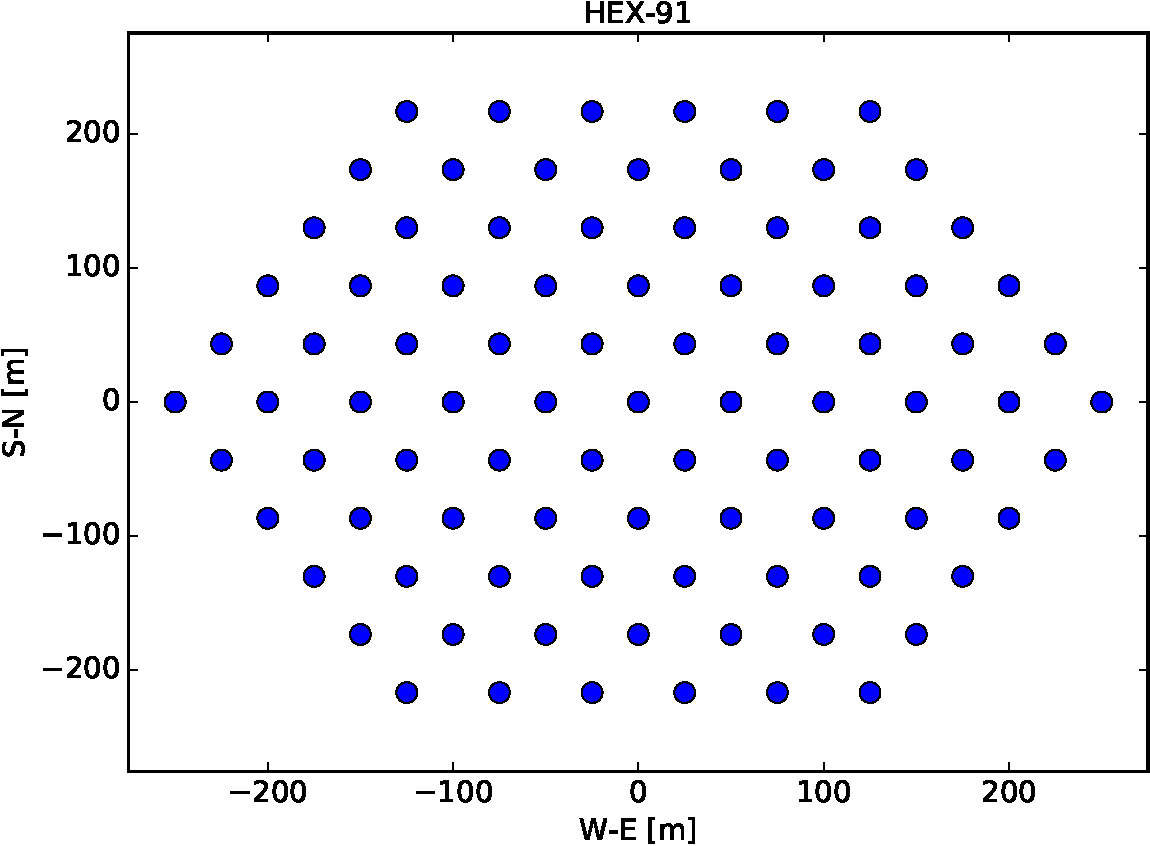
\includegraphics[width=0.32\textwidth]{./HEX_lay.pdf}\label{fig:HEX_lay}}
% \subfigure[Square layout]
% {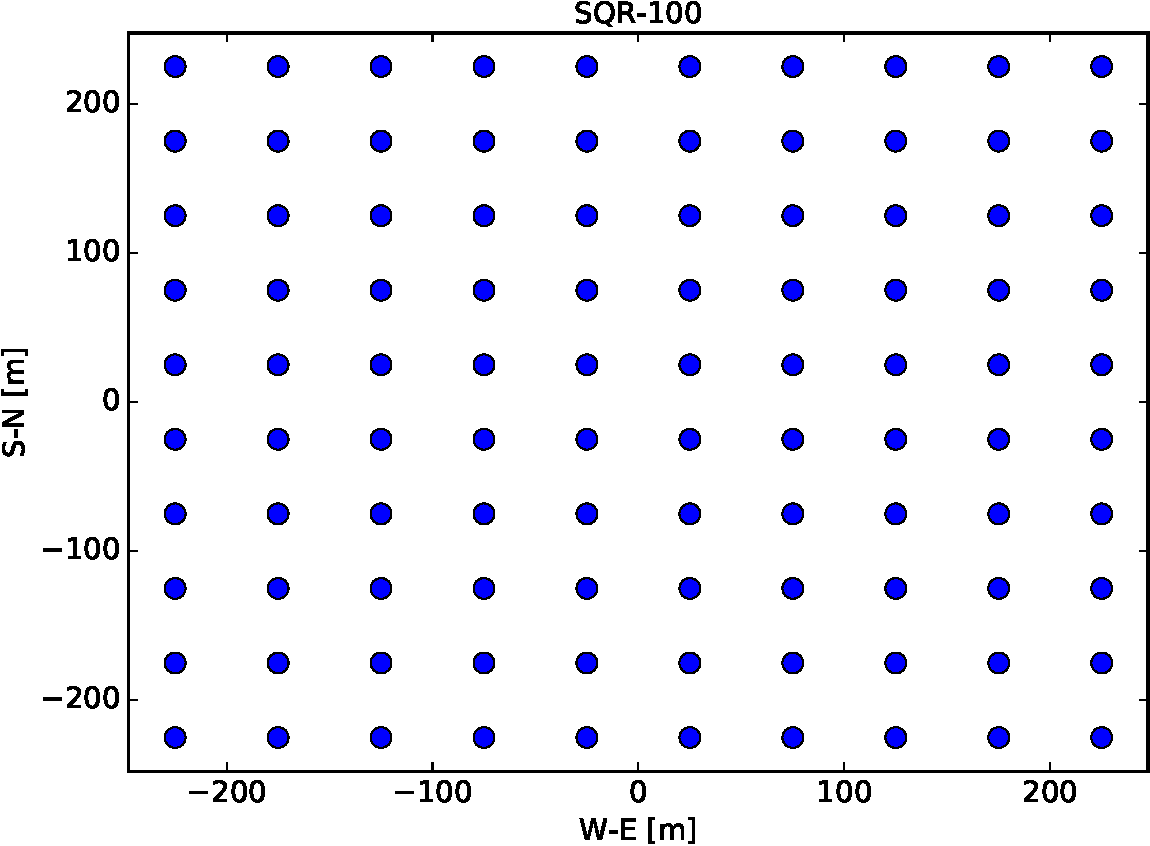
\includegraphics[width=0.32\textwidth]{./SQR_lay.pdf}\label{fig:SQR_lay}}
% \subfigure[Regular east-west layout]
% {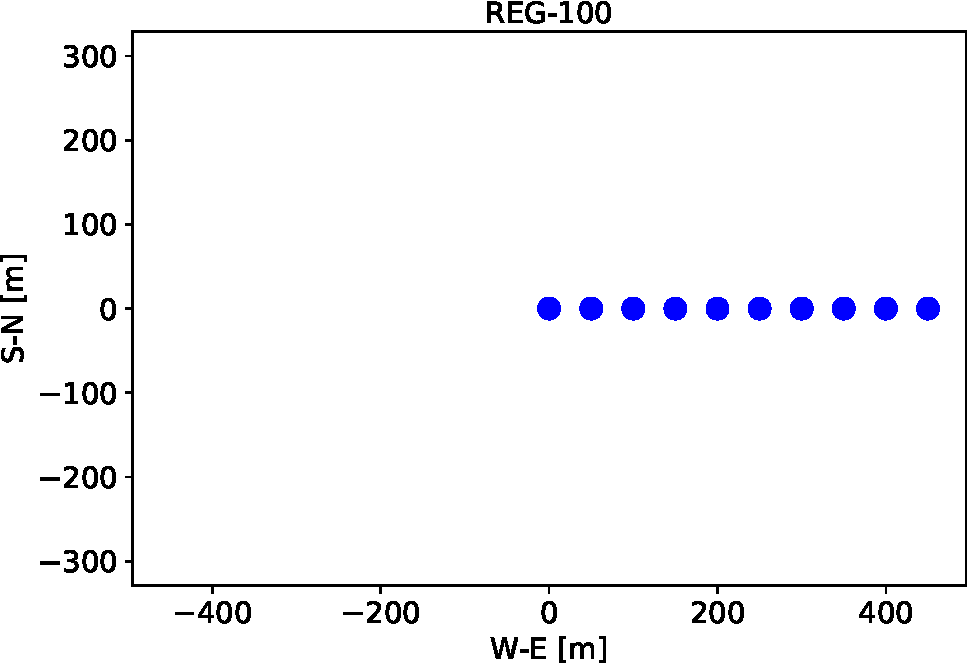
\includegraphics[width=0.32\textwidth]{./REG_lay.pdf}\label{fig:REG_lay}}
% 
% \subfigure[Hexagonal: $\zeta_{pq}$]
% {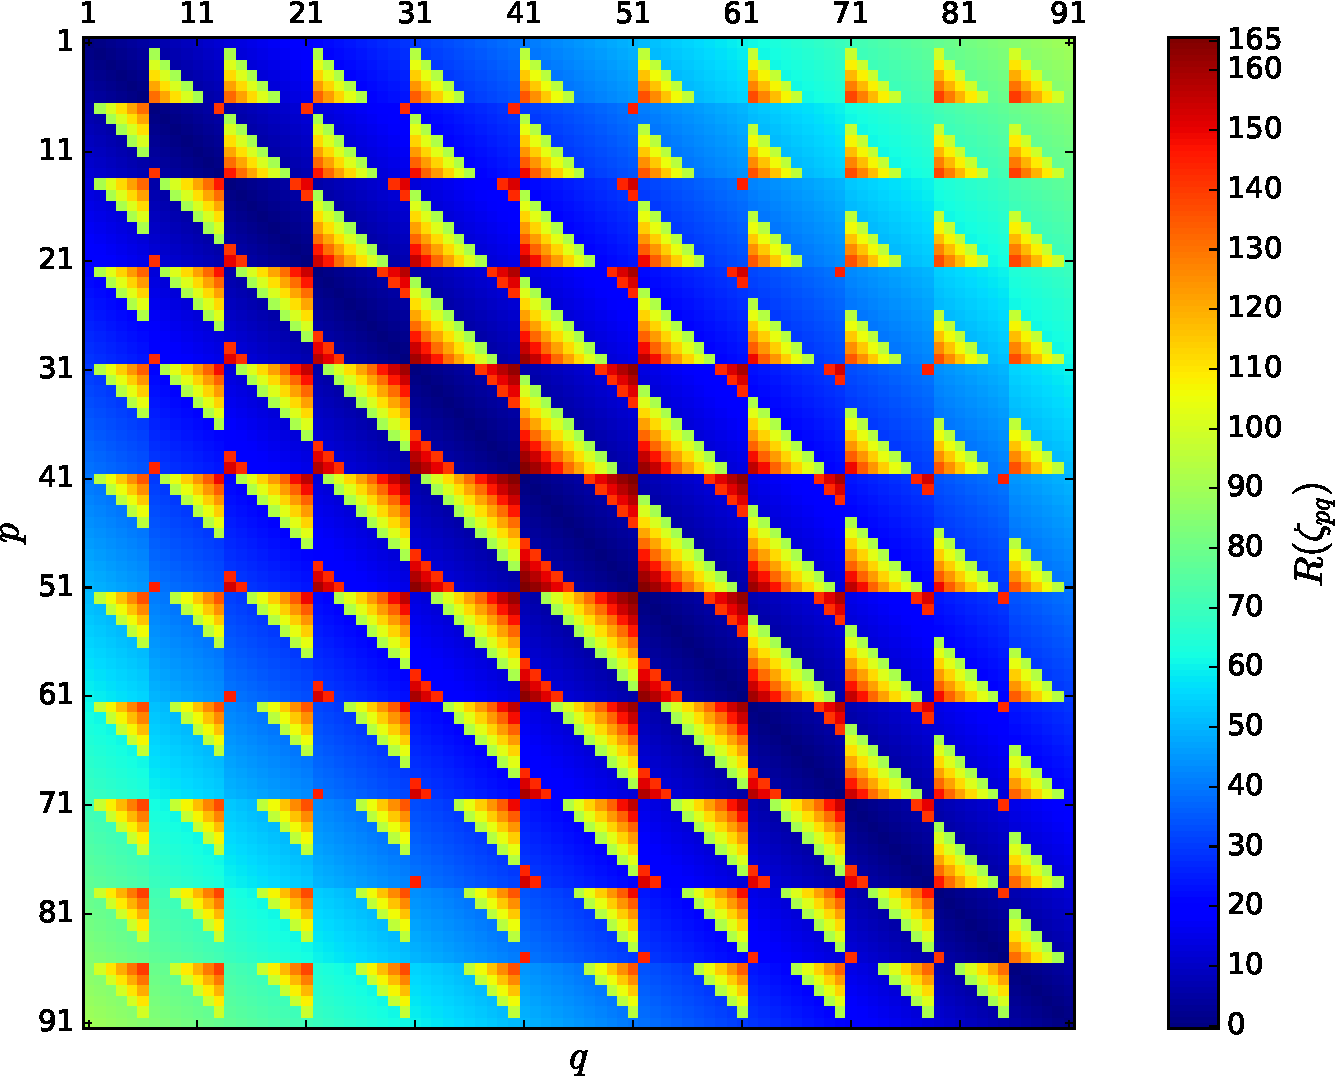
\includegraphics[width=0.33\textwidth]{./HEX_phi.pdf}\label{fig:HEX_phi}}
% \subfigure[Square: $\zeta_{pq}$]
% {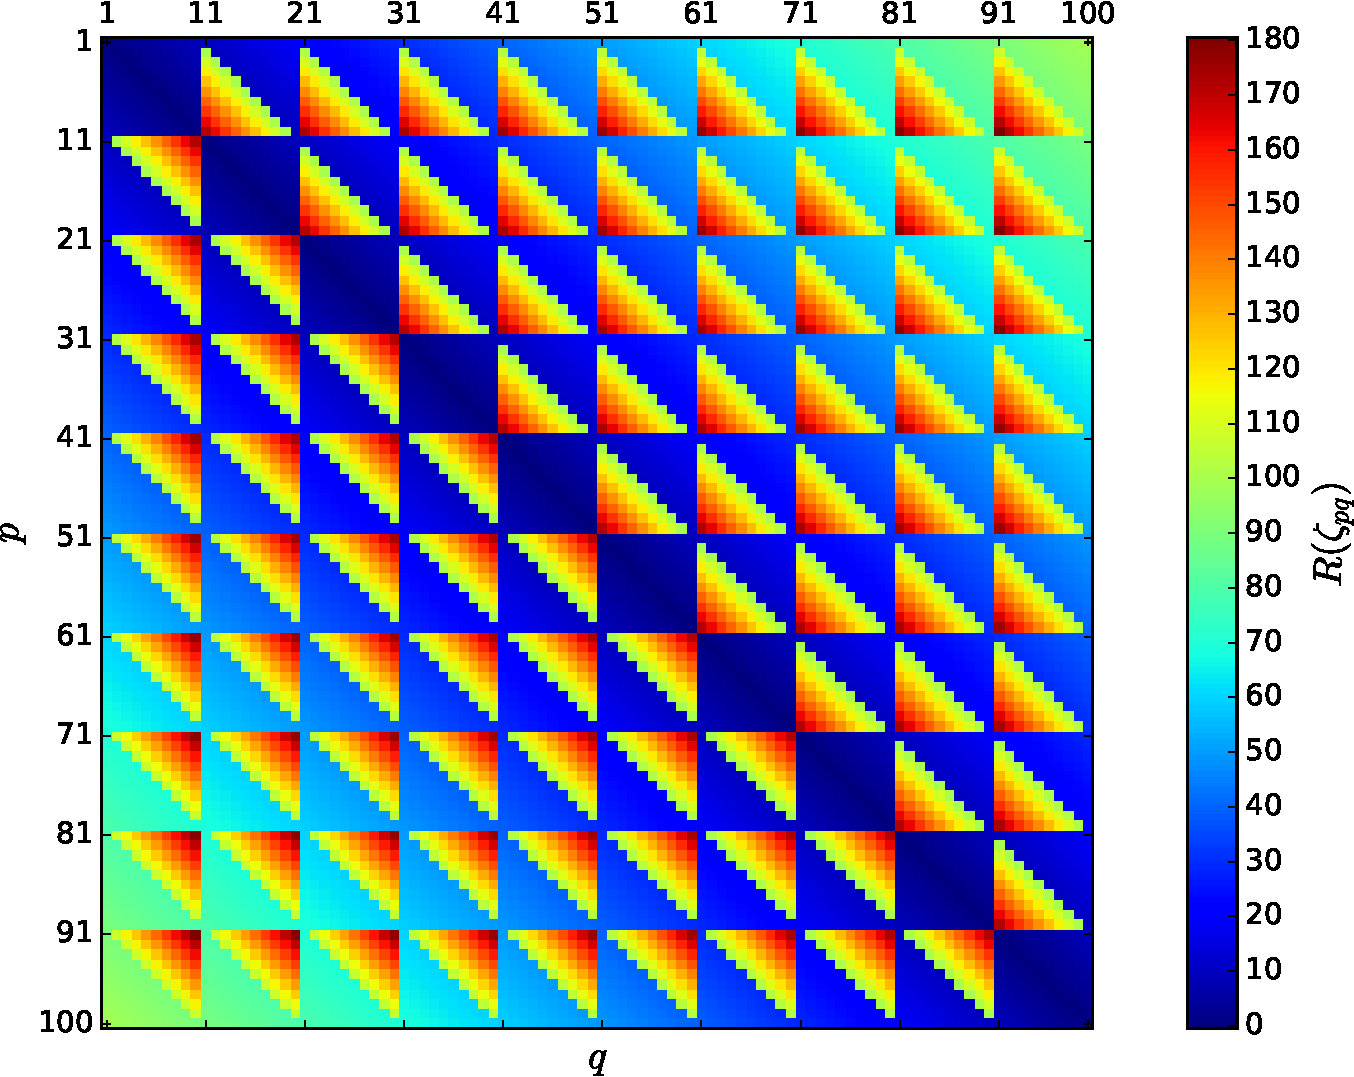
\includegraphics[width=0.33\textwidth]{./SQR_phi.pdf}\label{fig:SQR_phi}}
% \subfigure[Regular east-west: $\zeta_{pq}$]
% {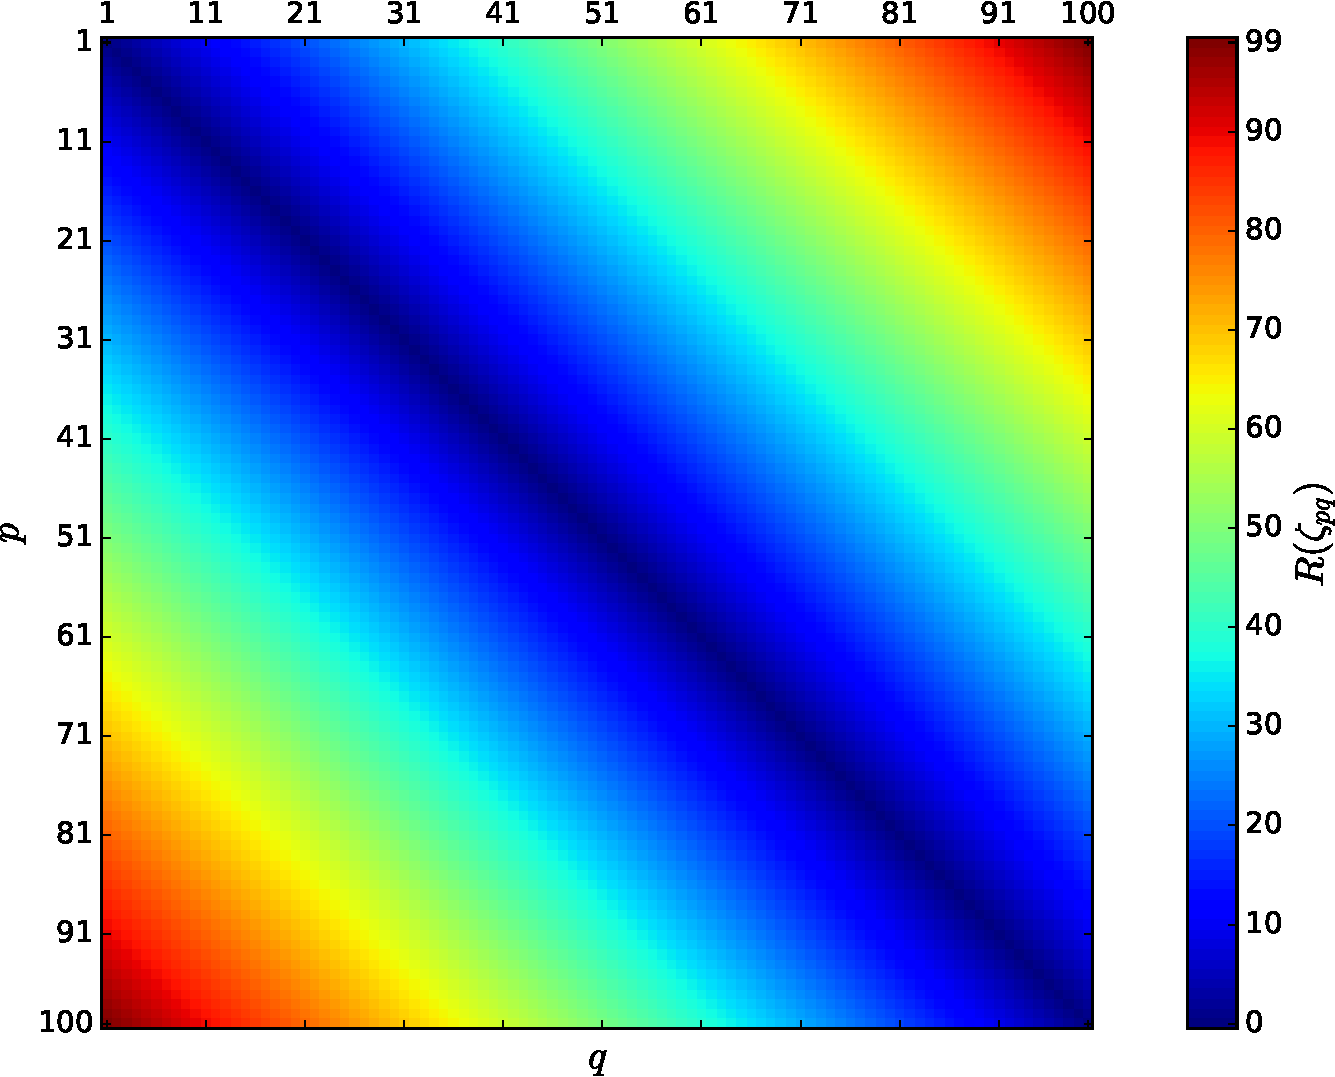
\includegraphics[width=0.33\textwidth]{./REG_phi.pdf}\label{fig:REG_phi}}
% \caption{In the top panel we have three different redundant antenna layouts, namely a hexagonal (left), square (middle) and a regular east-west (right) layout. 
% In the bottom panel we have the respective symmetric redundancy geometry functions for the layouts on the top panel. We used 91 antennas
% to construct the hexagonal layout, while 100 antennas where used in the square and east-west layouts. In the case of the east-west layout we only plot the positions of the first ten antennas. The maximal amount of redundant baseline groups that can be formed for 
% the hexagonal, square and east-west layouts are 165, 180 and 99 respectively.\label{fig:geometry_function}}
% \end{figure*}
% 
% If the function $\phi_{pq}$ is known and one is given one of the two antenna indexes that together form a redundant baseline as well as the redundant baseline group index itself then it is possible 
% to calculate the unknown antenna index. This can be computed via the following two expressions:
% \begin{equation}
% \xi_{ij} = 
% \begin{cases}
% p~\textrm{if}~\exists! ~ p \in \mathbb{N} ~ s.t. ~(\phi_{pi} = j)\\
% 0~\textrm{otherwise}
% \end{cases},
% \end{equation}
% and
% \begin{equation}
% \psi_{ij} = 
% \begin{cases}
% q~\textrm{if}~\exists! ~ q \in \mathbb{N} ~ s.t. ~(\phi_{iq} = j)\\
% 0~\textrm{otherwise}
% \end{cases}.
% \end{equation}
% We use $\xi_{ij}$ to retrieve the first antenna index of the composite antenna pair associated with a particular baseline, if the index of the first antenna in the composite antenna pair and the unique redundant baseline group index are known, while we use $\psi_{ij}$ to obtain 
% a similar result: the second antenna index of the composite antenna pair. %\textbf{NB::} I still need to plot $\zeta_{ij}$ for different antenna layouts.

\citet{Smirnov2015} realized that the diagonal entries of the Hessian matrix $\bH$ are much more significant than its off-diagonal entries, i.e. $\bH$ is nearly diagonal. By approximating $\bH$ by its diagonal and substituting the approximate Hessian matrix the LM parameter update step becomes \citep{Smirnov2015}:
\begin{align}
\breve{\bg}_{k+1} &\approx \frac{1}{1+\lambda}\widetilde{\bH}^{-1}\bJ^H\breve{\bd} + \frac{\lambda}{1+\lambda} \breve{\bg}_k,\label{eq:stef_lambda} \nonumber \\
 &= \alpha \widetilde{\bH}^{-1}\bJ^H\breve{\bd} + (1-\alpha)\breve{\bg}_k, \label{eq:stef_alpha}  
\end{align}
%\begin{align}
%\breve{\bg}_{k+1} &\approx \frac{1}{1+\lambda}\widetilde{\bH}^{-1}\bJ^H\breve{\bd} + \frac{\lambda}{1+\lambda} \breve{\bg}_k,\label{eq:stef_lambda}\\
% &= \alpha \widetilde{\bH}^{-1}\bJ^H\breve{\bd} + (1-\alpha)\breve{\bg}_k, \label{eq:stef_alpha}  
%\end{align}
where $\alpha = \frac{1}{1+\lambda}$. Note that equation~\ref{eq:one_half} and equation~\ref{eq:stef_alpha} are   
not dependent on $\breve{\br}$. 

Interestingly enough, if $\lambda = 0$ we obtain the odd parameter update step of \textsc{StEfCal}\footnote{$k\in\{0,2,\cdots\}$}, and if $\lambda=1$ (which corresponds
to $\alpha=\frac{1}{2}$) we obtain the even parameter update step of \textsc{StEfCal}\footnote{$k\in\{1,3,\cdots\}$} \citep[\textsc{StEfCal},][]{Mitchell:MWA-cal,Salvini2014}. In the \textsc{StEfCal} algorithm, the measurement equation, equation~\ref{eq:vis_definition}, is linearized by assuming that the gains are known, but that their conjugates are not. Under this assumption, the system of equations become linear and the conjugates of the gains can be obtained straightforwardly. Starting from the latest value of the gain conjugates, an updated estimate of the gains can be obtained and the succession continues until convergence is reached.
Alternating between solving and fixing different sets of parameters (which is exactly what \textsc{StEFCal} does) is in general referred to 
as the alternating direction implicit method (ADI). The \textsc{StEFCal} algorithm reduces the computational complexity of calibration from $\mathbb{O}(N^3)$ to $\mathbb{O}(N^2)$.

{\bf (GB: Trienko, I am not sure about where to place the paragraph below till the end of the subsection... probably because I'm not sure what ``even" and ``odd" \textsc{StEfCal} steps are... can we add the GN step after equation~\ref{eq:stef_lambda}???)}

{\bf (TLG: I have rewritten the above to make the odd and even stefcal steps more clear. I have also move the GN simplified equation before the 
stefcal explanation. GB to rewrite.)}


%A special case of solutions referred to as the alternating direction implicit \citep[ADI,][]{Salvini2014} algorithm is obtained by choosing $\lambda = 0$ \citep{Smirnov2015}. In particular, this choice of $\lambda$ is the parameter estimation step of the \textsc{StEfCal} algorithm \citep{Mitchell:MWA-cal,Salvini2014}, the most used implementation of ADI algorithms.  
%{\bf (GB: Trienko, I am not sure about where to place the paragraph below till the end of the subsection... probably because I'm not sure what ``even" and ``odd" \textsc{StEfCal} steps are... can we add the GN step after equation~\ref{eq:stef_lambda}???)}
%On the other hand, if we choose $\lambda$ equal to one (which corresponds
%to $\alpha=\frac{1}{2}$) we obtain the new parameter estimation step of \textsc{StEfCal} used during even iterations. Note the similarity between the last terms of equation~\ref{eq:stef_alpha} and equation~\ref{eq:one_half} when $\alpha$ is a half.
%Furthermore, the simplified skymodel-based GN equivalent of equation~\ref{eq:two_thrids} is equal to
%\citep{Smirnov2015}
%\begin{equation}
%\label{eq:one_half}
%\breve{\bg}_{k+1} = (\bJ^H\bJ)^{-1}\bJ^H\breve{\bd} + \frac{1}{2}\breve{\bg}_{k}. 
%\end{equation}
%Note that in equation~\ref{eq:one_half} the influence that the estimate of the parameters from the previous iteration has on the current iteration is scaled by a half, while
%in equation~\ref{eq:two_thrids} it is scaled by two thirds. 

%\subsection{Alternating Direction Implicit Method}
%\label{sec:adi}
%We start this section by briefly reviewing the ADI method as it pertains to skymodel-based calibration in Section~\ref{sec:sbc} \citep{Salvini2014,Smirnov2015}.
%
%In Section~\ref{sec:red_c}, we will show that the fast redundant calibration algorithm, that is presented in \citet{Marthi2014}, is in fact nothing more than an extension of the skymodel-based ADI method, presented in \citet{Salvini2014}, to the redundant calibration use case (i.e. redundant \textsc{StEfCal}). In doing so we will justify the naming convention we have been using for it.
%
%In Section~\ref{sec:adi_results}, we present some ADI simulation results. 
%
%\subsubsection{Skymodel-based Calibration}
%\label{sec:sbc}
%\textsc{StEfCal} is an ADI method in which the measurement equation, equation~\ref{eq:vis_definition}, is linearized by assuming that the gains are known, but that their conjugates are unknown \citep{Mitchell:MWA-cal,Salvini2014}. Under this assumption, the conjugates of the gains can be obtained trivially. Once the conjugates of the gains have been computed, it is possible to solve for the gains. One can then alternate between computing the gains and their conjugates until convergence is reached. By correctly exploiting the symmetry inherent in the calibration problem, this alternating approach can be replaced by a single iterative new parameter estimation step. \cite{Salvini2014} also show that the convergence of the algorithm can be improved, if for every even iteration, the basic new parameter estimation step is modified as follows: the current gain estimate is replaced by the average of the current gain estimate and the gain estimate of the previous odd iteration.
%\textsc{StEFCal} lowers the computational complexity of normal skymodel-based calibration from $\mathbb{O}(N^3)$ to $\mathbb{O}(N^2)$. 
%
%\citet{Smirnov2015} recently showed that one can also derive \textsc{StEFCal} by viewing normal skymodel-based calibration as a complex optimization problem. They realized while inspecting the skymodel-based $\bH$ that its diagonal entries are much more significant than its off-diagonal entries. As we mention in Section~\ref{sec:results}, the exact same conclusion can be reached if we inspect the Hessian $\bH$ that is associated with redundant calibration (see Fig.~\ref{fig:hessian}). By approximating the skymodel-based $\bH$ by its diagonal and substituting this approximate Hessian $\widetilde{\bH}$ back into the fundamental skymodel-based LM update step we obtain \citep{Smirnov2015} 
%\begin{align}
%\breve{\bg}_{k+1} &\approx \frac{1}{1+\lambda}\widetilde{\bH}^{-1}\bJ^H\breve{\bd} + \frac{\lambda}{1+\lambda} \breve{\bg}_k,\label{eq:stef_lambda}\\
% &= \alpha \widetilde{\bH}^{-1}\bJ^H\breve{\bd} + (1-\alpha)\breve{\bg}_k, \label{eq:stef_alpha}  
%\end{align}
%where $\alpha = \frac{1}{1+\lambda}$. Moreover, $\lambda = \frac{1-\alpha}{\alpha}$.
%
%If we choose $\lambda$ to be zero, which corresponds to an $\alpha$ equal to one, we obtain the new parameter estimation step of \textsc{StEfCal} used during odd iterations. On the other hand, if we choose $\lambda$ equal to one (which corresponds to $\alpha=\frac{1}{2}$) we obtain the new parameter estimation step of \textsc{StEfCal} used during even iterations. 
%
%Furthermore, the simplified skymodel-based GN equivalent of equation~\ref{eq:two_thrids} is equal to
%\citep{Smirnov2015}
%\begin{equation}
%\label{eq:one_half}
%\breve{\bg}_{k+1} = (\bJ^H\bJ)^{-1}\bJ^H\breve{\bd} + \frac{1}{2}\breve{\bg}_{k}. 
%\end{equation}
%Note that in equation~\ref{eq:one_half} the influence that the estimate of the parameters from the previous iteration has on the current iteration is scaled by a half, while in equation~\ref{eq:two_thrids} it is scaled by two thirds. Note the similarity between the last terms of equation~\ref{eq:stef_alpha} and equation~\ref{eq:one_half} when $\alpha$ is a half.




\section{Redundant Wirtinger Calibration}
\label{sec:red_wirtinger}
Interferometric baselines are named redundant when they sample the exact same visibilities in the $uv$-plane, i.e. if baseline $pq$ and $rs$ are redundant then $y_{pq} = y_{rs}$. It is convenient to group redundant visibilities together and label each group using a single index rather than using their antenna pairs as in equation~\ref{eq:vis_definition}. We introduce a function $\phi_{pq}$ that maps the antenna pair associated with a specific baseline to the single group index of the redundant baseline group that includes the baseline in question, i.e. if baseline $pq$ and $rs$ are redundant then $\phi_{pq} = \phi_{rs}$. 
The function $\phi_{pq}$ is not symmetric as $\phi_{pq} =
0$ if $p \geq q$. 
%Redundant baselines sample the exact same visibilities in the $uv$-plane, i.e. if baseline $pq$ and $rs$ are redundant then $y_{pq} = y_{rs}$. We can therefore group all the baselines that measure the exact same visibilities into the same redundant baseline group. We %index redundant baseline groups with single group indices instead of composite antenna pairs. 
%Let $\phi_{pq}$ be the function that maps the composite antenna pair associated with a specific baseline 
%
%to the single group index of the redundant baseline group to which the baseline in question belongs, i.e. if baseline $pq$ and $rs$ are redundant then $\phi_{pq} = \phi_{rs}$.  
%The function $\phi_{pq}$ is not symmetric as 
%$\phi_{pq} = 0$ if $p\geq q$. We can define the following symmetric variant of $\phi_{pq}$:
%\begin{equation}
%\zeta_{pq} = 
%\begin{cases}
%\phi_{pq}~\textrm{if}~p \leq q\\
%\phi_{qp}~\textrm{if}~p>q
%\end{cases}.
%\end{equation} 
Equation~\ref{eq:vis_definition} can be re-written for a redundant array as:
%If the array is redundant we can rewrite equation~\ref{eq:vis_definition} as
\begin{equation}
\label{eq:vis_red}
d_{pq} = g_{p}\conj{g_q}y_{\phi_{pq}} + n_{pq},
\end{equation}
with the same vector form as equation~\ref{eq:vis_red} if
%equation~\ref{eq:vis_red} can also be expressed in the following vector form 
%\begin{equation}
%\label{eq:vis_red_vec}
%\bd = \bv + \bn, 
%\end{equation}
%where 
\begin{align}
 \left [ \bd \right]_{\alpha_{pq}} &= d_{pq}, & \left [ \bv \right ]_{\alpha_{pq}} &= v_{pq}=g_p y_{\phi_{pq}} \conj{g_q},\nonumber\\
 \left [ \bn \right ]_{\alpha_{pq}} &= n_{pq}, &  &\label{eq:vec_definitions}
\end{align}
where the vectors in Equation~\ref{eq:vec_definitions} are column vectors of size $B$ (i.e. $p<q$).

We also introduce the following symmetric variant of $\phi_{pq}$:
\begin{equation}
\zeta_{pq} = 
\begin{cases}
\phi_{pq}~\textrm{if}~p \leq q\\
\phi_{qp}~\textrm{if}~p>q
\end{cases},
\end{equation} 
and we will refer to $\zeta_{pq}$ as the symmetric geometric function.
It is possible to construct a simple analytic expression for $\zeta_{pq}$ for an east-west regular array, i.e. $\zeta_{pq} = |q-p|$. It becomes, however, increasingly difficult to construct analytic expressions of $\zeta_{pq}$ for more complicated array layouts. The empirically constructed symmetric geometry functions of three different redundant layouts are displayed in Figure~\ref{fig:geometry_function}. We denote the range of $\zeta_{pq}$ with $\mathcal{R}(\zeta_{pq})$. The maximal element that $\zeta_{pq}$ can ascertain is denoted by $L$ and can be interpreted as the maximal number of unique redundant baseline groups which can be formed for a given array layout. 
%Alternatively, we can interpret the symmetric geometry functions in Fig.~\ref{fig:geometry_function} as geometry matrices. In this alternative paradigm, $\zeta_{pq}$ denotes a matrix entry. The dimension of these geometry matrices are $N\times N$.

\begin{figure*}
\centering
\subfigure[Hexagonal layout]
{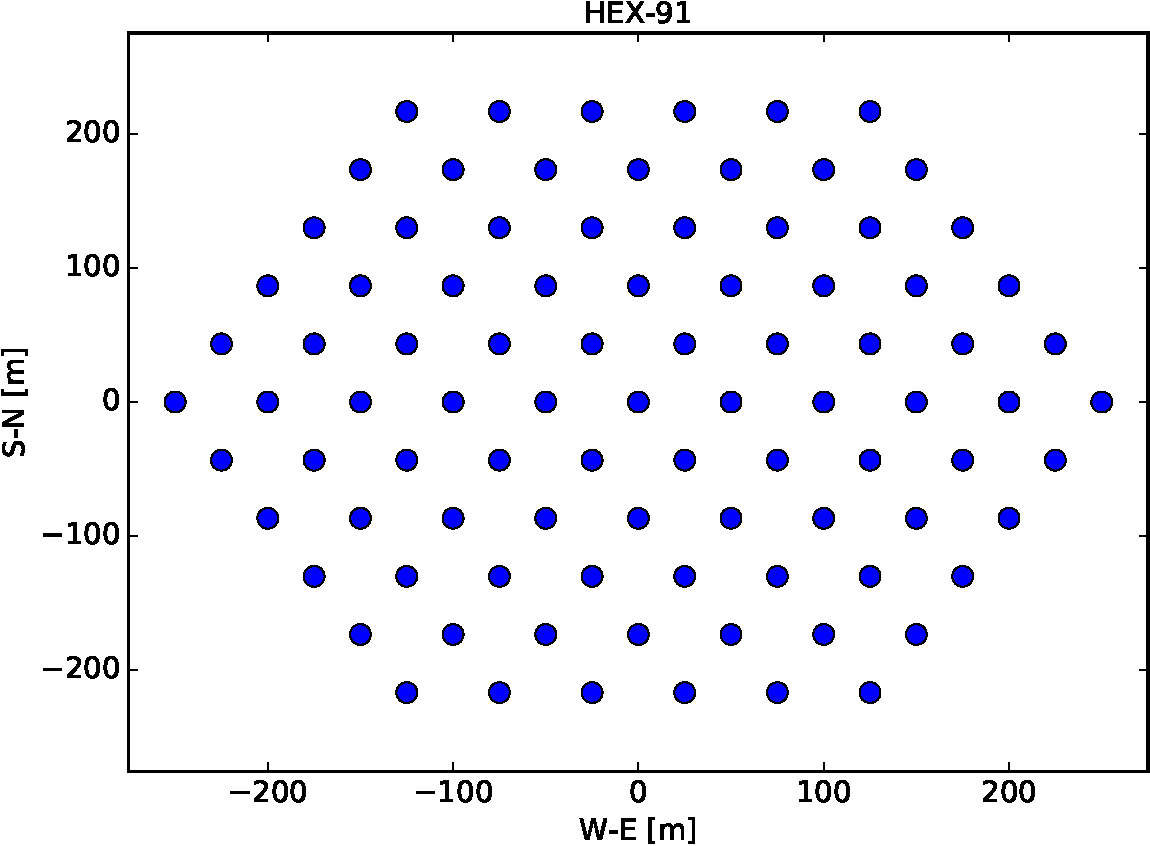
\includegraphics[width=0.32\textwidth]{./HEX_lay.pdf}\label{fig:HEX_lay}}
\subfigure[Square layout]
{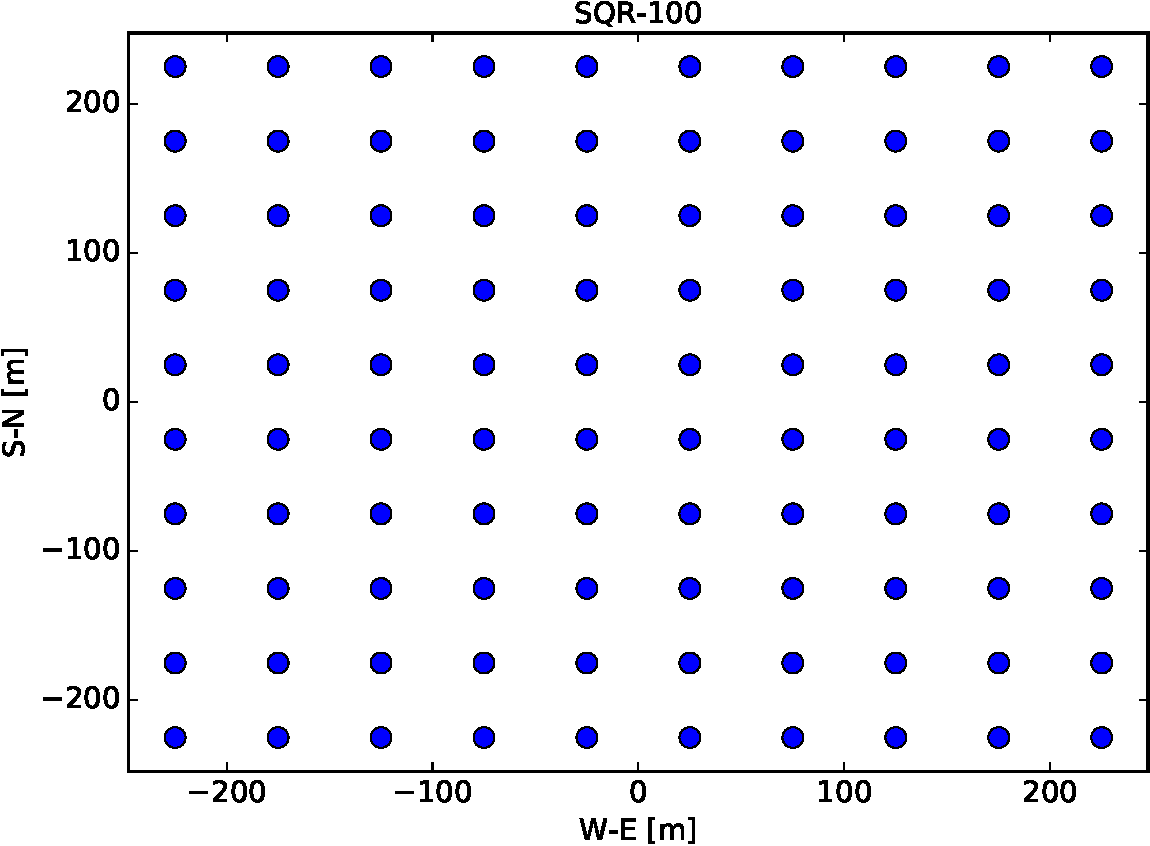
\includegraphics[width=0.32\textwidth]{./SQR_lay.pdf}\label{fig:SQR_lay}}
\subfigure[Regular east-west layout]
{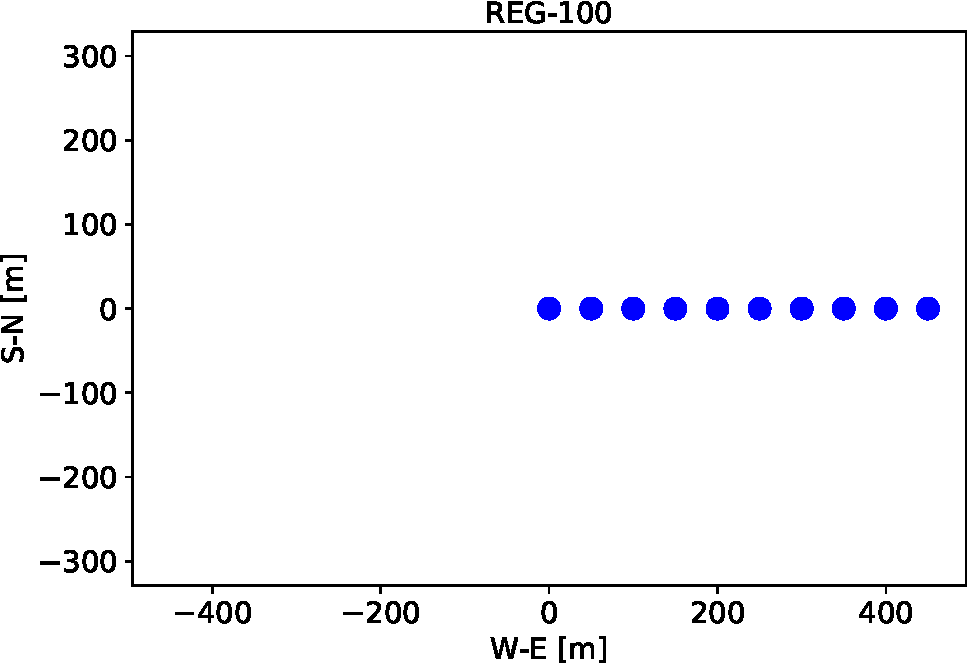
\includegraphics[width=0.32\textwidth]{./REG_lay.pdf}\label{fig:REG_lay}}

\subfigure[Hexagonal: $\zeta_{pq}$]
{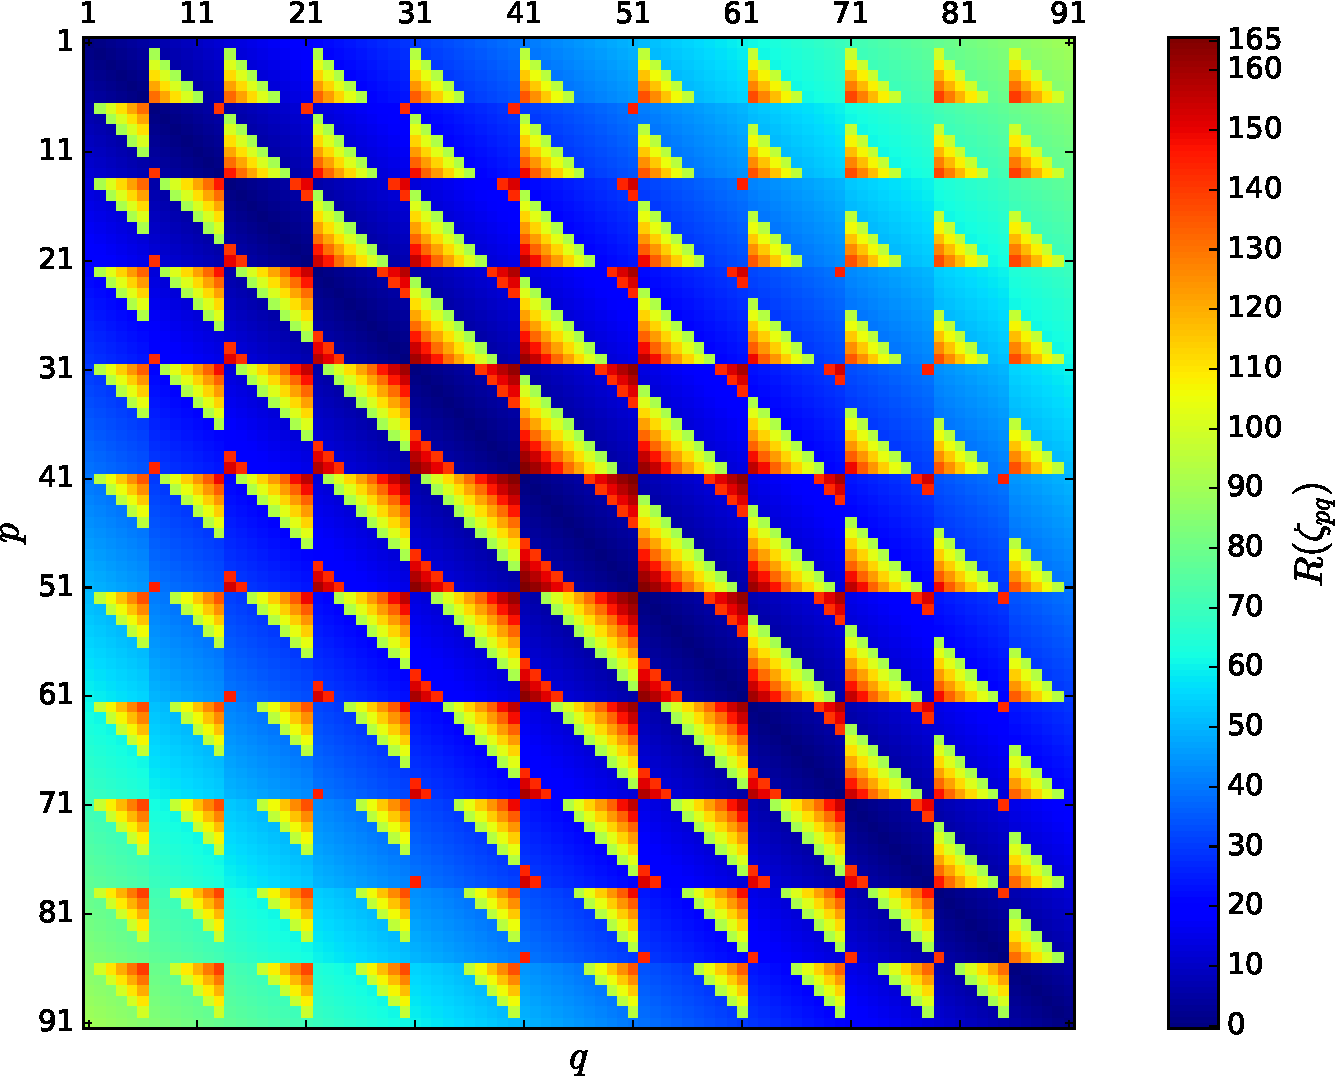
\includegraphics[width=0.33\textwidth]{./HEX_phi.pdf}\label{fig:HEX_phi}}
\subfigure[Square: $\zeta_{pq}$]
{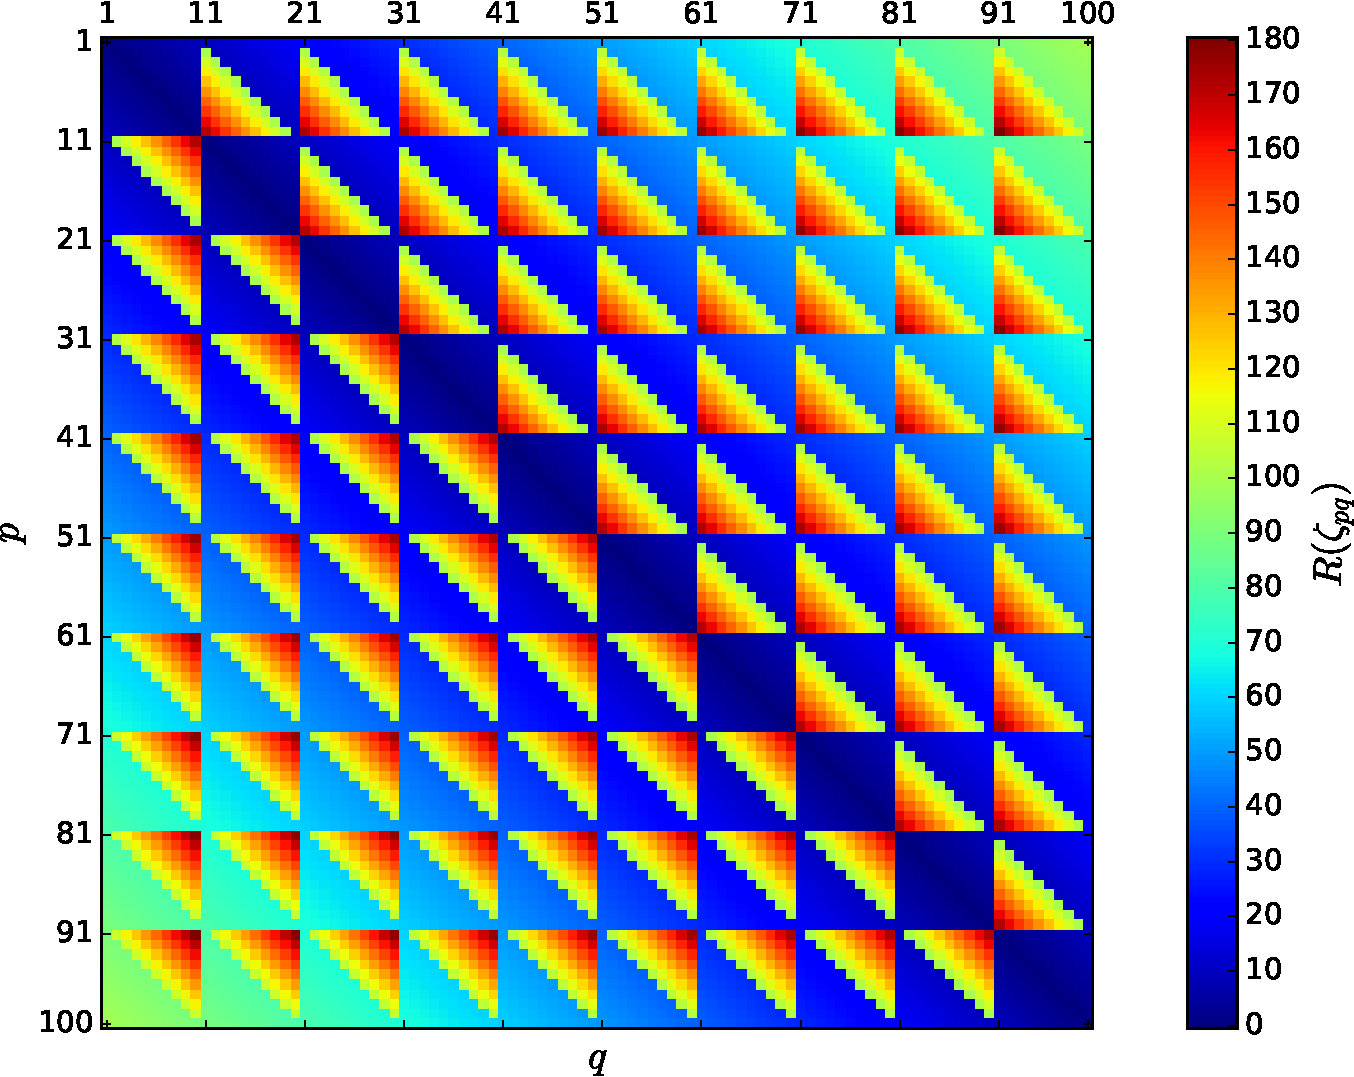
\includegraphics[width=0.33\textwidth]{./SQR_phi.pdf}\label{fig:SQR_phi}}
\subfigure[Regular east-west: $\zeta_{pq}$]
{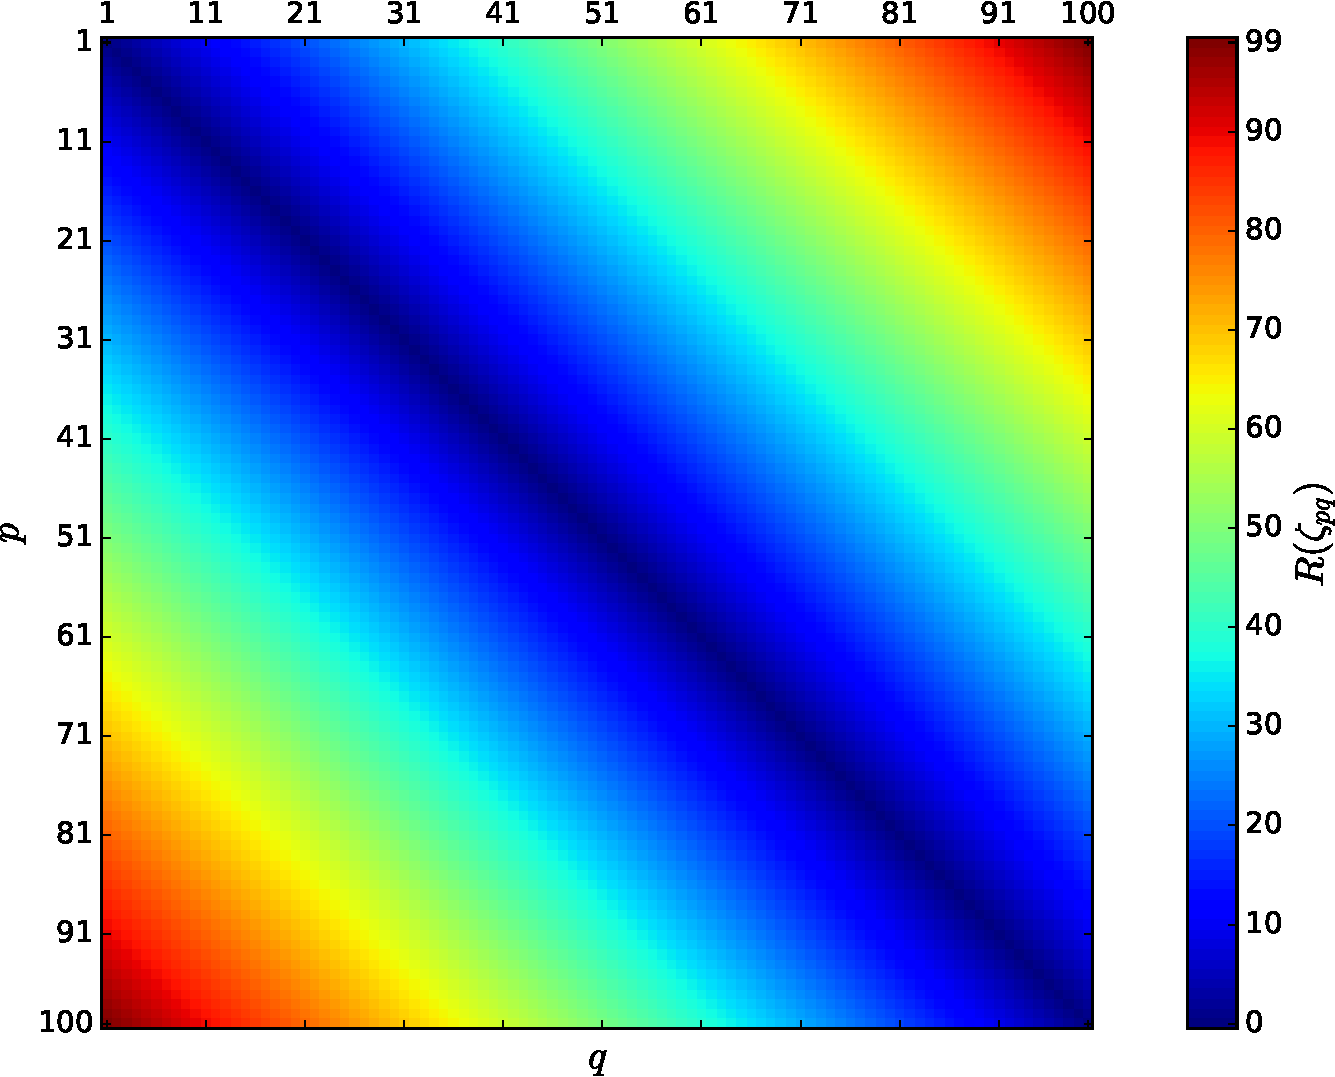
\includegraphics[width=0.33\textwidth]{./REG_phi.pdf}\label{fig:REG_phi}}
\caption{Three different redundant antenna layouts: hexagonal (top left), square (top middle) and regular east-west (top right) with their respective symmetric redundancy geometry functions $\zeta_{pq}$ (bottom panels). We used 91 antennas to construct the hexagonal layout, while 100 antennas were used in the square and east-west layouts. In the case of the east-west layout we only plot the positions of the first ten antennas. The maximal amount of redundant baseline groups $L$ that can be formed for 
the hexagonal, square and east-west layouts are 165, 180 and 99 respectively. The analytic expressions of $L$ for an hexagonal, square and east-west layout is $L = 2N-\frac{1}{2}\sqrt{12N-3}-\frac{1}{2}$,
$L=2N-2\sqrt{N}$ and $L=N-1$.\label{fig:geometry_function}}
\end{figure*}

We can now formulate redundant calibration as a least-squares problem:
\begin{equation}
\label{eq:least_squares_red}
\min_{\bz} \Lambda(\bz) = \min_{\bz} \|\br\|_F^2 = \min_{\bz} \|\bd - \bv(\bz)\|_F^2, 
\end{equation}
where
\begin{align}
 \bg &=[g_1,\cdots,g_N]^T, & \by &= [y_1,\cdots,y_L]^T,\nonumber\\
 \bz &= [\bg^T,\by^T]^T, &  &\label{eq:parm_definitions}
 \end{align}
where the number of model parameters to be solved of is now $P = 2(N+L)$, since redundant calibration is a complex problem.
{\bf (GB: is the following important? I thought it could be removed...) We plot $L$ and $P$ for two different geometric layouts in Fig~\ref{fig:pl}.
The analytic expressions for the red and the blue curve in Fig.~\ref{fig:ln} are \citep{Camps2003}
\begin{equation}
L = 2N-\frac{1}{2}\sqrt{12N-3}-\frac{1}{2} 
\end{equation}
and
\begin{equation}
L = N - 1 
\end{equation}
respectively.}

{\bf (TLG: Done.)}

%The number of model parameters that we need to solve for in equation~\ref{eq:least_squares_red} is $P = 2(N+L)$, since redundant calibration is a complex problem.

{\bf (TLG: This section got removed during a previous edit. It needs to be put back somewhere????)}

\subsection{Limitations}
 \label{sec:scope}
 We only deal with per-timeslot and frequency channel calibration. No solution smoothing  
 is applied between the different timeslots and channels. The reader interested in this is referred to \citep{Zheng2014}. 
 Moreover, we do not explicitly deal with any of the degeneracies normally associated with redundant calibration \citep{Zheng2014,Kurien2016}. Similar to the approach taken in \citep{Marthi2014}, we assume that the degeneracies present in the redundant calibration solutions are removed with a final round of skymodel-based calibration.

As mentioned in Section~\ref{sec:sky_wirtinger}, equation~\ref{eq:least_squares_red} can be solved by splitting the problem into its real and
imaginary parts and then solve for the real and imaginary parts of the unknown parameters separately \citep{Wieringa1992,Liu2010,Zheng2014}. In Appendix~\ref{sec:logcal} and~\ref{sec:lincal} we review this approach.
%As already alluded to in Section~\ref{sec:sky_wirtinger}, we can solve equation~\ref{eq:least_squares_red} in one of two ways. We can split the problem into its real and imaginary parts and then solve for the real and imaginary parts of the unknown parameters separately or we can employ the notion of Wirtinger derivatives. The former approach is discussed in Section~\ref{sec:ri}, while the latter approach is described in Section~\ref{sec:w}. 
%
%\subsection{Real and Imaginary Approach}
%\label{sec:ri}
%Using least-squares to solve complex problems can be problematic as $\bv$ needs to be analytic in its argument. In the case of equation~\ref{eq:least_squares_red}, \citet{Liu2010} circumvents this difficulty by splitting the problem into its phase-and-amplitude components.
%
%The aforementioned is achieved by first rewriting equation~\ref{eq:least_squares_red} as
%\begin{equation}
%\label{eq:least_squares_lincal}
%\min_{\bmath{\varrho}} \|\breve{\br}\| = \min_{\bmath{\varrho}} \|\breve{\bd} - \breve{\bv}(\bmath{\varrho})\|, 
%\end{equation}
%where $\breve{\bd} = [\bd^T,\conj{\bd}^T]^T$, $\breve{\bv} = [\bv^T,\conj{\bv}^T]^T$ and $\bmath{\varrho}$ is the phase and amplitude parameter vector which we define in Appendix~\ref{sec:lincal}. 
%With the aid of equation~\ref{eq:least_squares_lincal} we can derive the algorithm implemented in \textsc{lincal} (see Appendix~\ref{sec:lincal}). The Jacobian associated with equation~\ref{eq:least_squares_lincal} is equal to equation~\ref{eq:Jac_lin}. Appendix~\ref{sec:lincal} makes it evident that \textsc{lincal} is equivalent to a basic GN update step \citep{Kurien2016}. 
%Therefore, a straightforward way of improving the convergence properties of stock standard \textsc{lincal} would be to simply add the LM damping factor to the basic \textsc{lincal} update step.
%In doing so the need to use $\textsc{logcal}$ before $\textsc{lincal}$ becomes superfluous. The use of $\textsc{logcal}$ may, however, still offer a computational advantage, as it is a very fast method to obtain a good starting solution, and would reduce the number of iterations needed by the LM algorithm. Proper experiments would need to be conducted to determine whether it is worth keeping $\textsc{logcal}$ in the algorithmic hierarchy. 
%
%\subsection{Wirtinger Approach}
%\label{sec:w}
%
%\citet{Smirnov2015} recently proposed to use the Wirtinger derivative instead of the classic real and imaginary approach to perform normal skymodel-based calibration. We will now show
%that the Wirtinger derivative can also be applied to redundant calibration.
%We can perform redundant calibration by solving the following optimization problem: 
%\begin{equation}
%\label{eq:least_squares_red}
%\min_{\bz} \Lambda(\bz) = \min_{\bz} \|\br\|_F^2 = \min_{\bz} \|\bd - \bv(\bz)\|_F^2, 
%\end{equation}
%where $\bz = [\bg,\by]^T$. The other vectors in equation~\ref{eq:least_squares_red} were defined in Section~\ref{} \footnote{In this paper we use the same symbol to denote corrupted predicted visibilities and true observed corrupted visibilities as it
%is trivial to distinguish which one is implied from the context. Using the same symbol for these two quantities improves the readability of the paper.}. Note the similarity between equation~\ref{eq:least_squares} and equation~\ref{eq:least_squares_red},
%i.e. redundant calibration can be cast as a non-linear least squares problem. 

We, instead, intend to formulate the redundant calibration problem using Wirtinger calculus. We therefore recast equation~\ref{eq:least_squares_red} as
%Analogous to \cite{Smirnov2015}, we recast equation~\ref{eq:least_squares_red} to 
\begin{equation}
\label{eq:least_squares_complex}
\min_{\breve{\bz}} \|\breve{\br}\| = \min_{\breve{\bz}} \|\breve{\bd} - \breve{\bv}(\breve{\bz})\|, 
\end{equation}
where $\breve{\bz} = [\bz^T,\conj{\bz}^T]^T$. 
%Equation~\ref{eq:least_squares_complex} is the complex conjugate augmented counterpart of equation~\ref{eq:least_squares_red}.
%The fact that $\bv$ is now analytic in its argument has the immediate consequence: it becomes possible to apply complex GN
%and complex LM to equation~\ref{eq:least_squares_complex}. 
We derive the complex Jacobian associated with equation~\ref{eq:least_squares_complex} to be:
%\subsubsection{Complex GN and LM}
%\label{sec:complex_GN_LM}
%The complex Jacobian associated with equation~\ref{eq:least_squares_complex} is equal to
\begin{equation}
\label{eq:Jacobian}
\bJ = \begin{bmatrix}
       \bmJ & \bmJ^*\\
       \conj{\bmJ}^* & \conj{\bmJ} 
      \end{bmatrix},
\end{equation}
where 
\begin{equation}
[\bmJ]_{\alpha_{pq},i} = \begin{cases} 
     \frac{\partial v_{pq}}{\partial g_i} & \textrm{if}~i\leq N \\
     \frac{\partial v_{pq}}{\partial y_{i-N}} & \textrm{otherwise}  
\end{cases}, %, & \bmJ^* &= \frac{\partial \bv}{\partial \conj{\bz}}. 
\end{equation}
and
\begin{equation}
[\bmJ^*]_{\alpha_{pq},i} = \begin{cases} 
     \frac{\partial v_{pq}}{\partial \conj{g}_i} & \textrm{if}~i\leq N \\
     \frac{\partial v_{pq}}{\partial \conj{y}_{i-N}} & \textrm{otherwise}  
\end{cases}. %, & \bmJ^* &= \frac{\partial \bv}{\partial \conj{\bz}}. 
\end{equation}
We can now calculate the GN and LM update steps to be 
%The GN update step is now defined as:
\begin{equation}
\label{eq:GN_update}
\Delta \breve{\bz} = (\bJ^H\bJ)^{-1}\bJ^H\breve{\br}
%\Delta \breve{\bz} &=& (\bJ^H\bJ + \lambda\bD)^{-1}\bJ^H\breve{\br},
\end{equation}
and 
%The LM update rule is defined in a very similar way:
\begin{equation}
\label{eq:LM_update}
\Delta \breve{\bz} = (\bJ^H\bJ + \lambda\bD)^{-1}\bJ^H\breve{\br},
\end{equation}
respectively. As in Section~\ref{sec:sky_wirtinger}, equation~\ref{eq:GN_update} can be used to iteratively update our parameter vector:
%we can now use equation~\ref{eq:GN_update} or equation~\ref{eq:LM_update} to iteratively update our parameter vector as follows:
\begin{equation}
\label{eq:update}
\breve{\bz}_{k+1} = \breve{\bz}_{k} + \Delta \breve{\bz}_{k}. 
\end{equation}
The analytic expressions for $\bJ$, $\bH$ and $\bJ^H\breve{\br}$ can be found in Appendix~\ref{sec:analytic}.

In the case of the GN algorithm we can simplify equation~\ref{eq:update} even further to obtain
\begin{equation}
\label{eq:two_thrids}
\breve{\bz}_{k+1} = (\bJ^H\bJ)^{-1}\bJ^H\breve{\bd} + \frac{2}{3}\breve{\bz}_{k}. 
\end{equation}
The above equation is derived in Appendix~\ref{sec:simplify_GN}. Equation~\ref{eq:two_thrids} is the redundant equivalent of equation~\ref{eq:one_half} and it shows us that in the case of redundant calibration we can calculate the GN parameter update step without calculating the residual.  

\begin{figure*}
\centering
\subfigure[Regular layout]{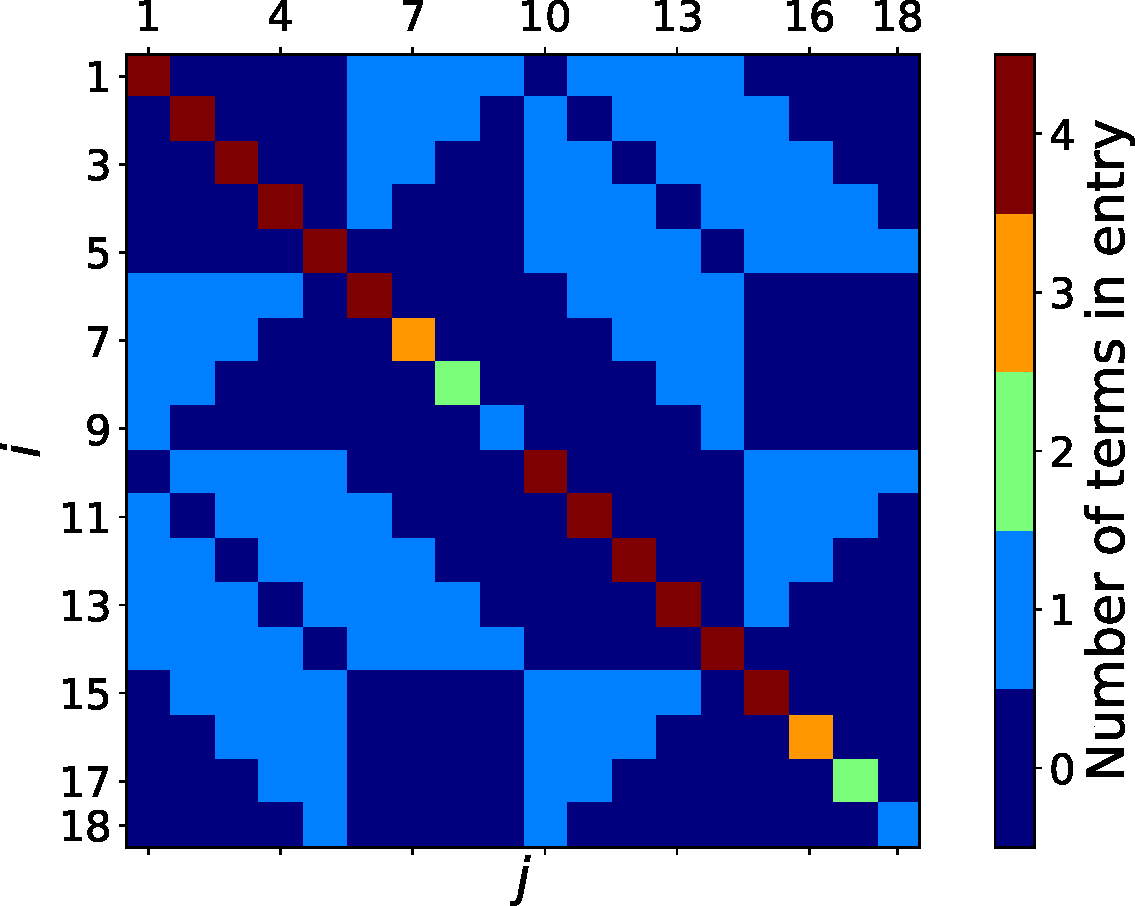
\includegraphics[width=0.47\textwidth]{./reg_hessian.pdf}\label{fig:hessian_reg}}
% V_R_3.pdf: 585x441 pixel, 72dpi, 20.64x15.56 cm, bb=0 0 585 441
\subfigure[Hexagonal layout]{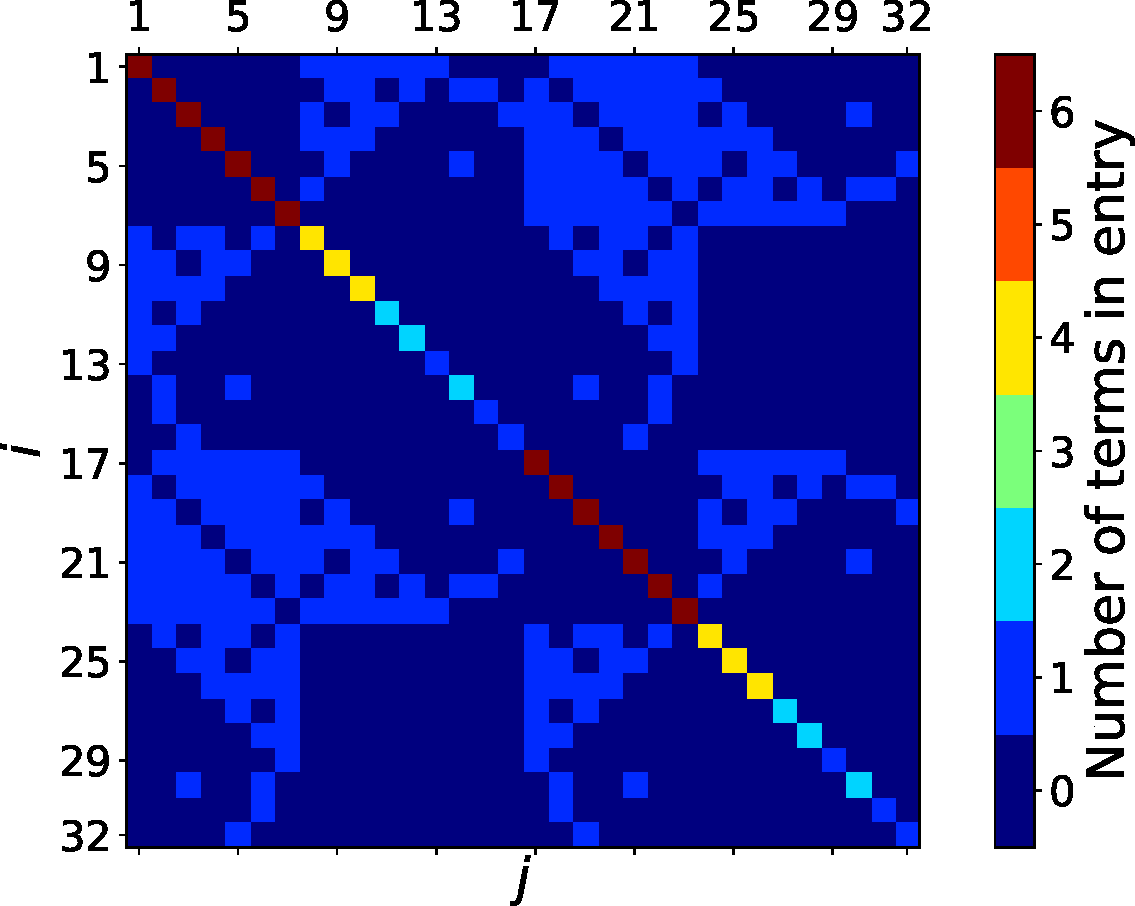
\includegraphics[width=0.47\textwidth]{./hex_hessian.pdf}\label{fig:hessian_hex}}
\caption{The number of analytic terms out of which the entries of the Hessian $\bH$ consist for two different geometric layouts, namely a regular east-west grid with $N = 5$ (left panel) and 
a hexagonal grid with $N = 7$. The diagonal entries of these two Hessians are clearly more significant than their off-diagonal entries. Moreover, these two Hessians also 
contain many zero-entries. Note that the locations of the zero-entries are dependent on the geometry of the array layout.
\label{fig:hessian}} 
\end{figure*}

Figure~\ref{fig:hessian} shows that the Hessian matrix $\bH$ is nearly diagonal and sparse for both a regular and hexagonal layout considered. We therefore follow the approach of \citet{Smirnov2015} and approximate the Hessian matrix $\bH$ with its diagonal. If we substitute $\bJ^H\bJ$ with $\widetilde{\bH}=\bH\odot\bI$ and replace $\breve{\br}$ with $\breve{\bd} - \breve{\bv}$ in equation~\ref{eq:GN_update} we obtain:
\begin{equation}
\label{eq:appr_GN}
 \Delta \breve{\bz} \approx \widetilde{\bH}^{-1}\bJ^H(\breve{\bd}-\breve{\bv})
\end{equation}
Utilizing the second identity in equation~\ref{eq:identities} allows us to simplify equation~\ref{eq:appr_GN} to
\begin{equation}
  \Delta \breve{\bz} \approx \widetilde{\bH}^{-1}\bJ^H\breve{\bd}-\breve{\bz},
\end{equation}
which leads to
\begin{equation}
 \breve{\bz}_{k+1} \approx \widetilde{\bH}^{-1}\bJ^H\breve{\bd}.
\end{equation}
We obtain a similar result if we repeat the above procedure, only in this case we use equation~\ref{eq:LM_update} instead. Thus,
\begin{align}
\breve{\bz}_{k+1} &\approx \frac{1}{1+\lambda}\widetilde{\bH}^{-1}\bJ^H\breve{\bd} + \frac{\lambda}{1+\lambda} \breve{\bz}_k,\label{eq:lambda}\\
 &= \alpha \widetilde{\bH}^{-1}\bJ^H\breve{\bd} + (1-\alpha)\breve{\bz}_k. \label{eq:alpha}  
\end{align}
The analytic expression of $\bJ^H\breve{\bd}$ will be very similar to the analytic 
expression of $\bJ^H\breve{\br}$, the only difference being that in equation~\ref{eq:ab} the letter $r$ would be replaced by a $d$. If we substitute the analytic expression
of $\bJ^H\breve{\bd}$ and $\widetilde{\bH}^{-1}$ (which can easily be constructed using Appendix~\ref{sec:analytic}) into equation~\ref{eq:alpha} we obtain the following two update rules:
\begin{equation}
\label{eq:g_update}
g_{i}^{k+1} = \alpha \frac{\sum_{j\neq i} g_j^k \widetilde{y}_{ij}^{~\!\!k} d_{ij}}{\sum_{j\neq i} |g_j^k|^2|y_{\zeta_{ij}}^k|^2} + (1-\alpha) g_i^k, 
\end{equation}
and
\begin{equation}
\label{eq:y_update}
y_{i}^{k+1} = \alpha \frac{\sum_{pq \in \mathcal{PQ}_i} \conj{g}_p^k g_q^k d_{pq}}{\sum_{pq \in \mathcal{PQ}_i}|g_p^k|^2|g_q^k|^2} + (1-\alpha) y_i^k. 
\end{equation}
The computational complexity of inverting $\widetilde{\bH}$ is $\mathbb{O}(P)$. We note that equation~\ref{eq:g_update} is the gain estimator associated with \textsc{StEfCal} and that equation~\ref{eq:g_update} and~\ref{eq:y_update} correspond to the parameter estimators derived by \citet{Marthi2014}.
In \citet{Marthi2014}, equation~\ref{eq:g_update} and~\ref{eq:y_update} are derived by taking the
derivative of the objective function $\Lambda$ relative to the elements of $\bg$ and $\by$, setting the intermediate results to zero and then solving
for the unknown parameters. The above two equations can also be derived using the ADI method. Please see Appendix~\ref{sec:red_stef_ADI} for the details. We will refer to the above parameter update steps as redundant \textsc{StEFCal} in the remainder of the 
paper.   

{\bf (GB: derived in which way? It would be useful to say in order to differentiate from us)}.
{\bf (TLG: Added)}.

The choice of $\alpha$ is somewhat unconstrained. 
In this paper we chose $\alpha=\frac{1}{3}$ (i.e. $\lambda = 2$) and we based our decision on the choice of $\alpha$ in the 
case of classic \textsc{StEFCal}. In the case of \textsc{StEFCal}, $\alpha = \frac{1}{2}$ (for even iterations),
which results in the last term of equation~\ref{eq:one_half} and equation~\ref{eq:stef_alpha} being equal. 
When $\alpha=\frac{1}{3}$, the last term of equation~\ref{eq:two_thrids} and equation~\ref{eq:alpha} are equal.

{\bf (GB: is this true? TRIENKO, I MANAGED TO REACH ONLY TILL THIS POINT. I THINK IT IS TIME I HAND THIS BACK TO YOU AND YOU MAKE AN EFFORT TO TIE IT UP. i THINK WE CAN GO FROM HERE TO A MINOR REVISION NEXT TIME)}
{\bf (TLG: tried to rephrase is it clear now?}


%In this paper we follow the same choice done in \textsc{StEFCal}, leading to $\alpha = 1/3$. The following simulations show this choice to be appropriate {\bf (GB: is this true? TRIENKO, I MANAGED TO REACH ONLY TILL THIS POINT. I THINK IT IS TIME I HAND THIS BACK TO YOU AND YOU MAKE AN EFFORT TO TIE IT UP. i THINK WE CAN GO FROM HERE TO A MINOR REVISION NEXT TIME)} 

%equation~\ref{eq:g_update} and equation~\ref{eq:y_update} are the exact same iterative new parameter estimators derived by \citet{Marthi2014}. Also note that equation~\ref{eq:g_update} is the fundamental gain estimator associated with skymodel-based \textsc{StEfCal}. We have, therefore, successfully used the diagonal approximation approach proposed by \citet{Smirnov2015} to re-derive the fast redundant calibration method presented in  \citet{Marthi2014}. 
%The question now arises what value should we use for $\alpha$? In \citet{Marthi2014}, they propose 
%$\alpha = 0.3$. Although an exact mathematical proof for the optimal choice of $\alpha$ still eludes us, it is still possible to
%venture a clever guess by studying what the choice of $\alpha$ is in the case of skymodel-based \textsc{StEFCal}. The value of $\alpha$ is equal to a half 
%in the case of \textsc{StEFCal} (for even iterations); see Section~\ref{sec:sbc}. If we wish to mimic this behaviour for the redundant calibration use case we need to scale $\breve{\bz}$ by two thirds in equation~\ref{eq:alpha} (see equation~\ref{eq:two_thrids}) which implies that we should choose $\alpha$ equal to a third, which corresponds to a $\lambda$ equal to two.
%We used this $\lambda$ value in this paper. The following simulation results show that this choice produces 
%good results.

Optimality results of redundant \textsc{StEFCal} were presented in \citet{Marthi2014}. We do not repeat their analysis here. We do, however, present our own redundant \textsc{StEFCal} results, in Fig.~\ref{fig:prec_error}, which confirm that the $\alpha$ value proposed 
in this paper produce accurate parameter estimates. To quantify the exact error in our estimates we used the percentage error $\beta$ defined 
as 
\begin{equation}
\label{eq:beta}
\beta = \frac{\|\bv - \widehat{\bv}\|_F^2}{\|\bv\|_F^2}.
\end{equation}
We have already defined $\bv$ in equation~\ref{eq:vec_definitions}. Moreover, in equation~\ref{eq:beta}, $\widehat{\bv}$ denotes the parameter estimate obtained with redundant \textsc{StEFCal}.

\begin{figure}
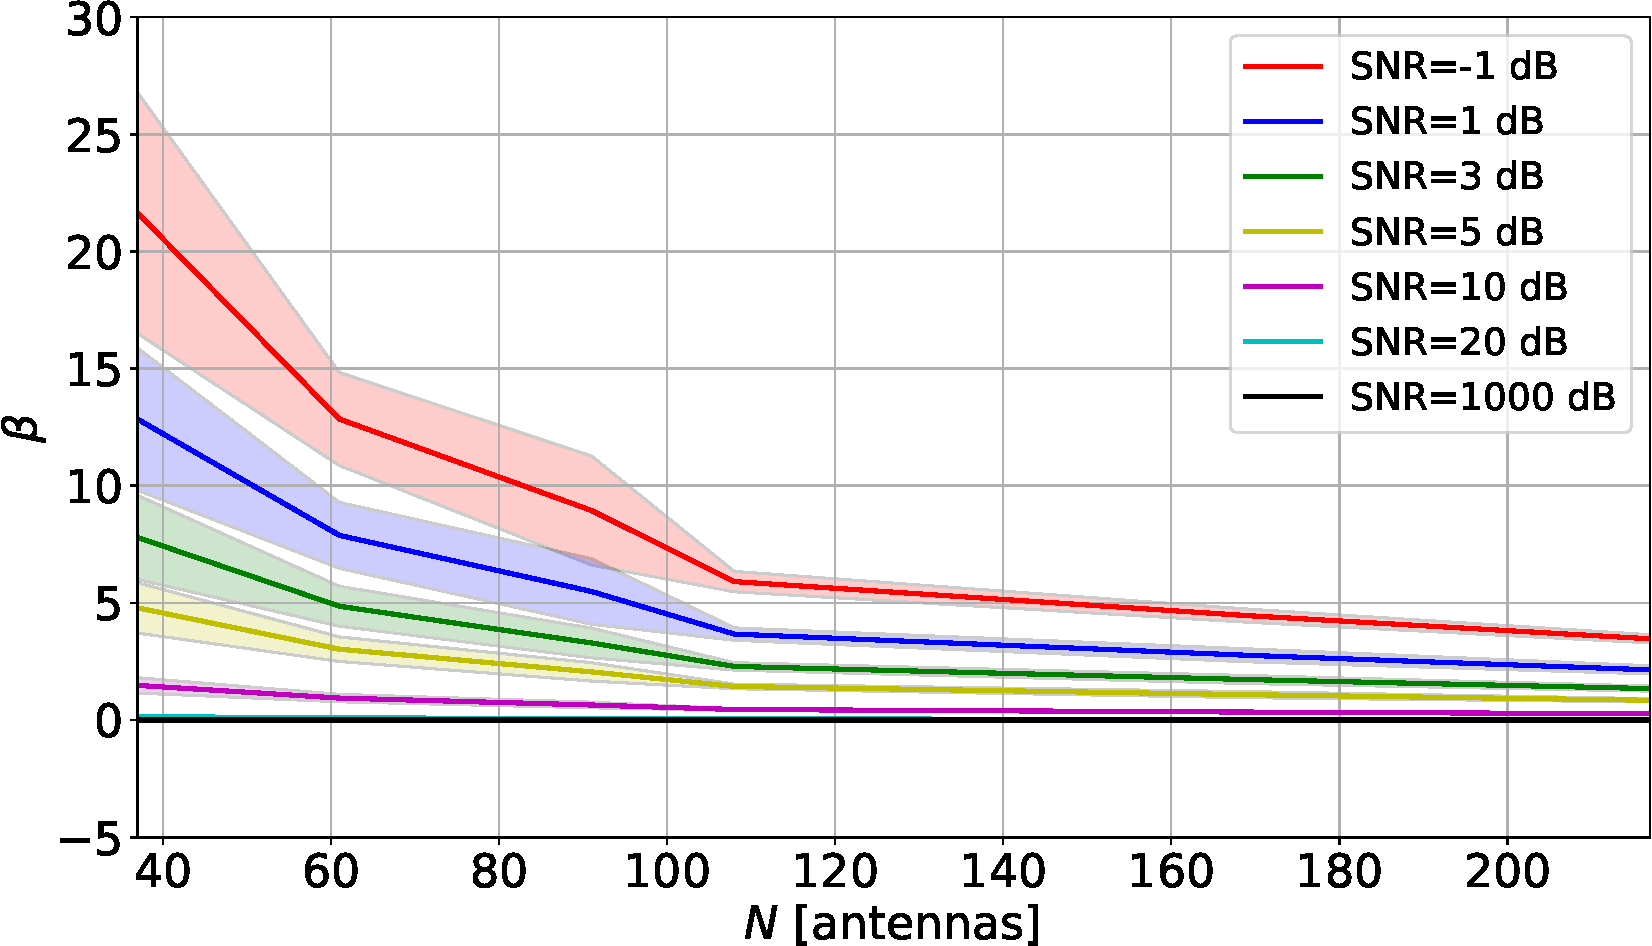
\includegraphics[width=0.47\textwidth]{./prec_error.pdf} 
\caption{We plot the percentage error $\beta$ between the estimated 
predicted visibilities and the true predicted visibilities for different SNR values as a function of the number of antennas in the array $N$. The graph presented here was generated using the first experimental setup in Table~\ref{tab:ch_parm}.}
\label{fig:prec_error}
\end{figure}


\section{Preconditioned Conjugate Gradient Method}
\label{sec:pcg}
In this section we investigate the computational complexity of the PCG method when applied to the redundant calibration problem. 
We briefly review the PCG method in Appendix~\ref{sec:conj_grad}. If the reader is not that familiar with the PCG method we encourage 
the reader to briefly review Appendix~\ref{sec:conj_grad} before continuing with the paper. The PCG method can be used to efficiently invert Hermitian sparse 
matrices, which is exactly the kind of matrix $\bH$ is (see Fig.~\ref{fig:hessian} and Eq.~\ref{eq:red_H}). There are two factors which influence the computational complexity of the PCG method, namely the spectral condition number $\kappa$ and the sparsity of the matrix we wish to invert (see equation~\ref{eq:cg_bound}). 

We investigate the spectral condition number and the sparsity of the modified Hessian $\bmH$ (i.e. $\lambda = 2$), which is a non-singular matrix, in Section~\ref{sec:scn} and Section~\ref{sec:sparsity} respectively.
It is interesting to note, that the Hessian $\bH$ itself is singular (from empirical tests) and that the PCG method 
can in principal be be used to pseudo-invert it (see Appendix~\ref{sec:normal}).

\subsection{Spectral Condition Number}
\label{sec:scn}
The convergence properties of the conjugate gradient (CG) algorithm can be dramatically improved through preconditioning. Inspecting Fig.~\ref{fig:hessian}, reveals that the Jacobian preconditioner
is a good candidate for the redundant use case. In Fig.~\ref{fig:kappa}, we see that this choice of preconditioner performs very well, the value of the spectral condition number $\kappa$
becomes constant and independent of problem size, i.e. the number of antennas in the array. Preconditioning therefore effectively eliminates $\kappa$ from equation~\ref{eq:cg_bound}. This result
is confirmed by Fig.~\ref{fig:cg_itr}. Fig.~\ref{fig:cg_itr} shows us that the number of major iterations needed by the preconditioned conjugate gradient method to invert $\bmH$ is independent of the number of antennas in the array.
Moreover, the number of major iterations required is also much smaller than the dimension of $\bmH$. 

%kappa + itr plots
\begin{figure*}
\centering
\subfigure[$\kappa$]{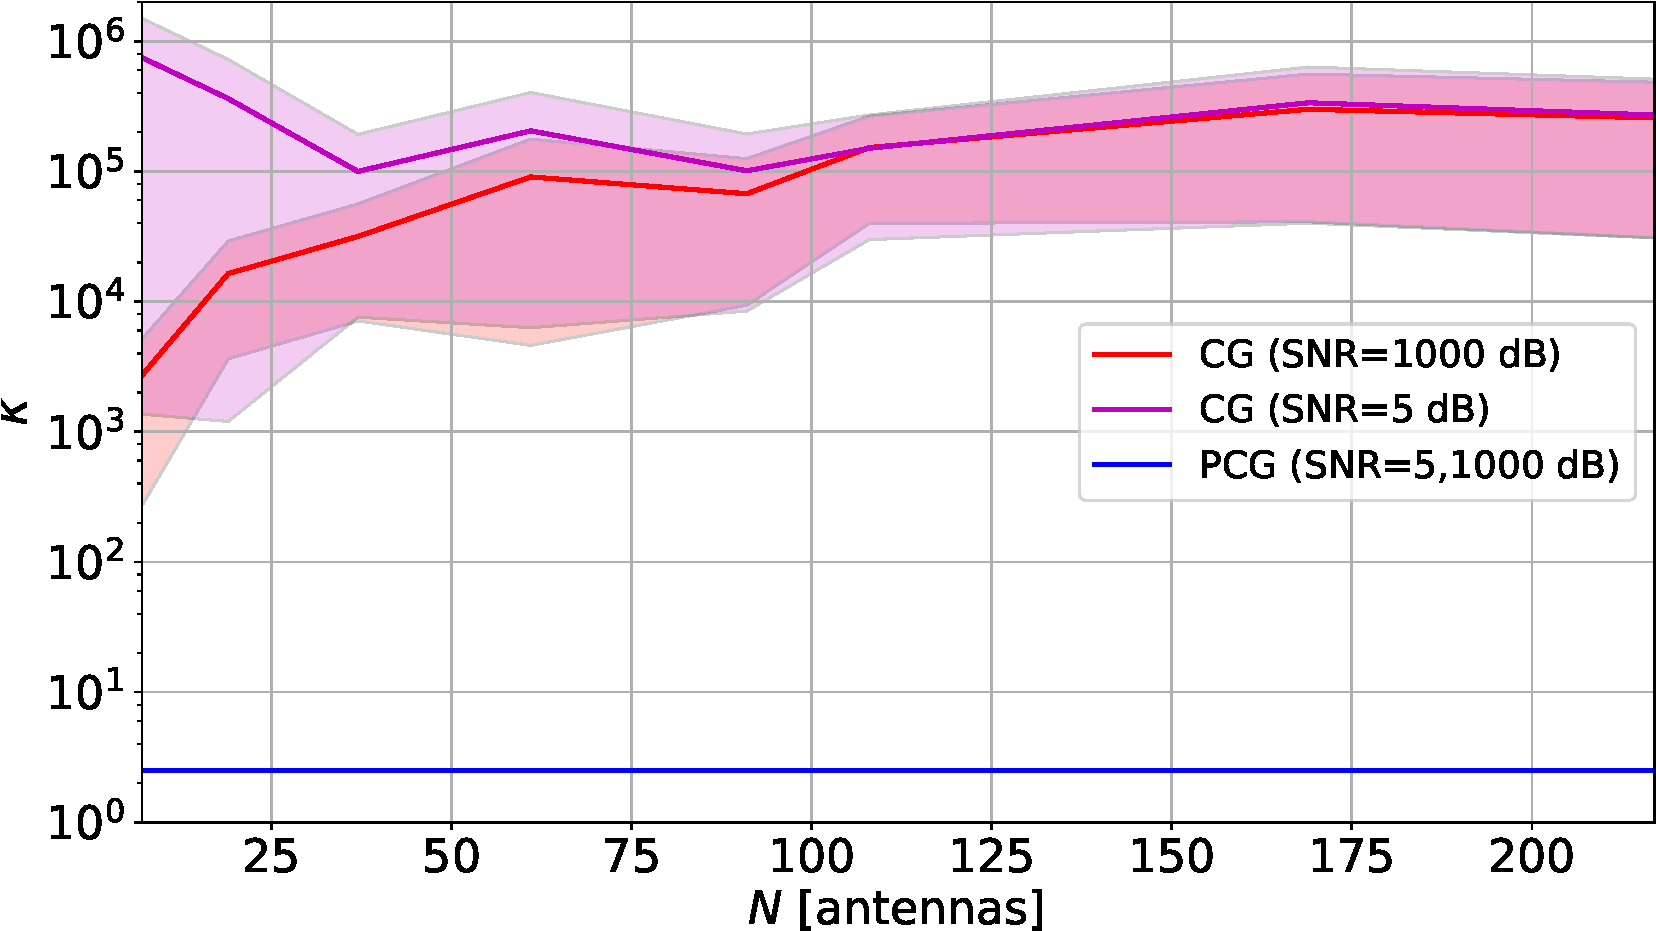
\includegraphics[width=0.47\textwidth]{./kappa.pdf}\label{fig:kappa}}
% V_R_3.pdf: 585x441 pixel, 72dpi, 20.64x15.56 cm, bb=0 0 585 441
\subfigure[Iterations required before and after Preconditioning]{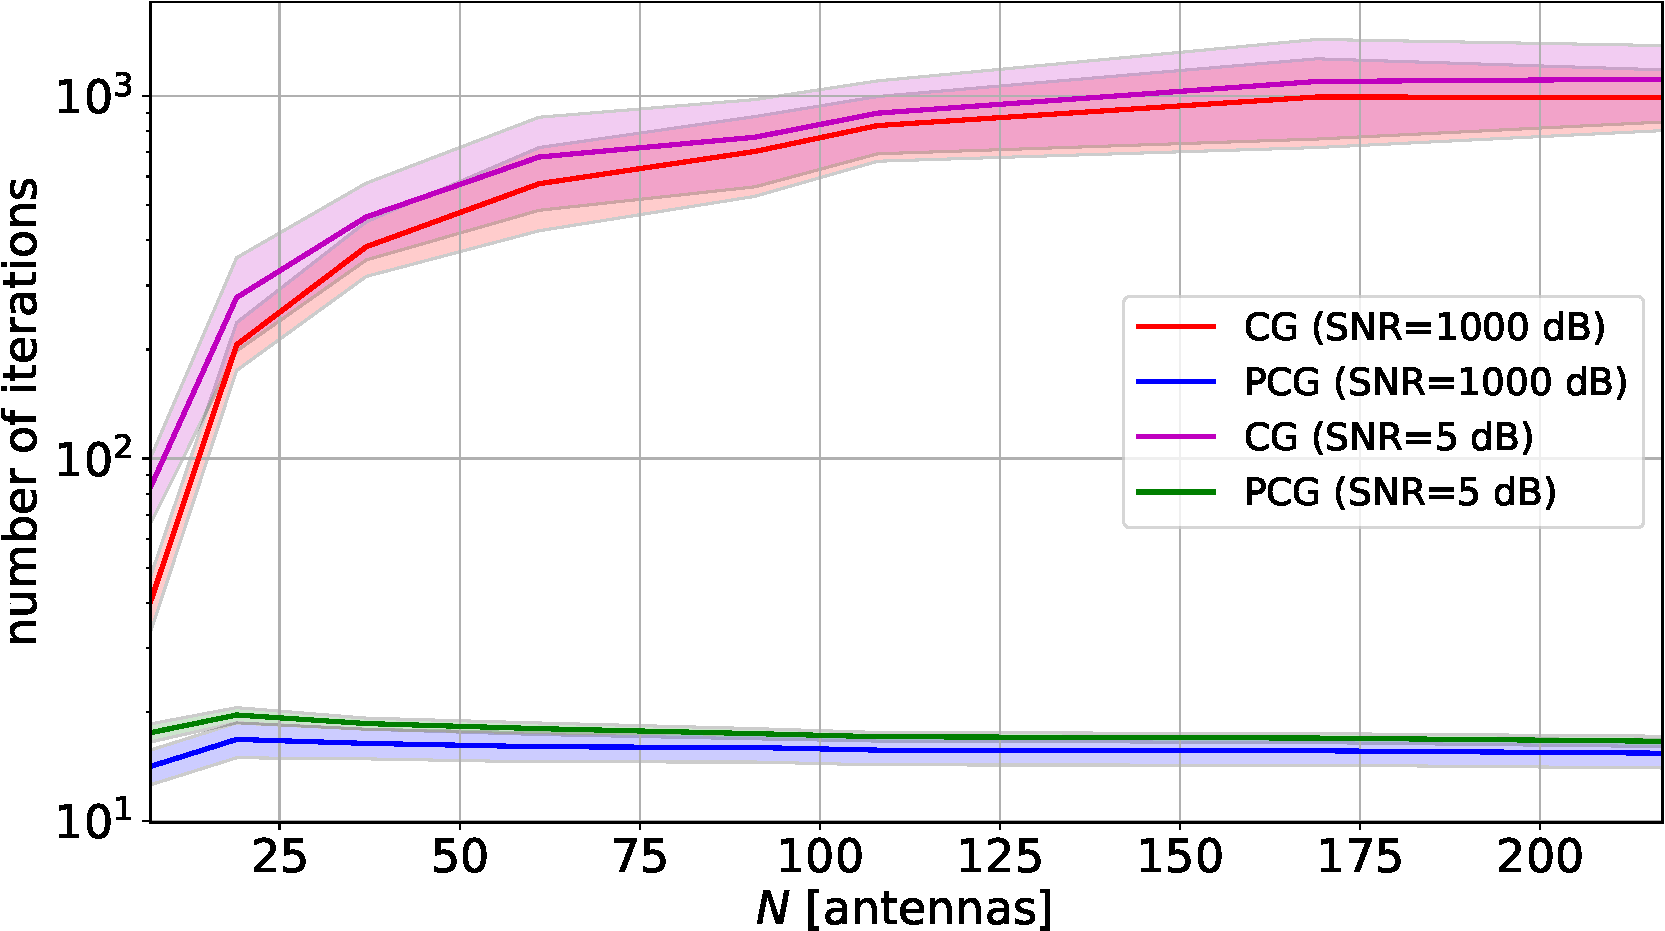
\includegraphics[width=0.47\textwidth]{./cg_itr.pdf}\label{fig:cg_itr}}
\caption{The graphs presented here were generated using the second experimental setup in Table~\ref{tab:ch_parm}. In the left panel we have plotted the spectral condition number $\kappa$ of the modified Hessian $\bmH$, before (magenta and red curves) and after preconditioning (blue curve), at different SNR values as a function of the
number of antennas $N$ in the array. The right hand panel confirms this result. In the right hand panel we have plotted the number of major iterations (line 6 of Algorithm \ref{algo:CG}) required by the conjugate 
gradient method to invert $\bmH$, before (magenta and red curves) and after preconditioning (blue and green curves), at different SNR values as a function of the number of antennas $N$ in the array.   
\label{fig:kappa_itr}} 
\end{figure*}

\subsection{Sparsity}
\label{sec:sparsity}
% \begin{enumerate}
% \item $\boldsymbol{H}$: is a $(4N-2)\times(4N-2)$ or a $P \times P$ matrix. $N$ denotes the number of antennas and $P$ denotes the number of parameters. This matrix
% contains $6N^2 - 2N - 2$ non-zero entries. It contains $16N^2 - 16N + 4$ entries. We can construct this matrix with $4N^2 -  4N$ or $\frac{1}{4} P^2 -1$ elementary operations.
% \item $\boldsymbol{A}$: is a $(2N-1)\times(2N-1)$ matrix. This matrix has $N^2 + N - 1$ non-zero entries. We can construct this matrix with $2\frac{1}{2} (N^2 -  N)$ elementary operations.  
% \item $\boldsymbol{B}$: is a $(2N-1)\times(2N-1)$ matrix. This matrix has $2N^2 - 2N$ non-zero entries. We can construct this matrix with $1\frac{1}{2} (N^2 -  N)$ elementary operations.
% \item $\boldsymbol{C}$: is a $N\times N$ matrix. This matrix has $N$ non-zero entries. We can construct this matrix with $N^2-N$ elementary operations.
% \item $\boldsymbol{D}$: is a $N \times (N-1)$ matrix. This matrix has $\frac{1}{2} (N^2 -  N)$ non-zero entries. We can construct this matrix with $\frac{1}{2} (N^2 -  N)$ elementary operations. 
% \item $\boldsymbol{E}$: is a $(N-1) \times (N-1)$ matrix. This matrix has $(N-1)$ non-zero entries. We can construct this matrix with $\frac{1}{2} (N^2 -  N)$ elementary operations.  
% \item $\boldsymbol{F}$: is a $N \times N$ matrix. This matrix has $N^2 - N$ non-zero entries. We can construct this matrix with $\frac{1}{2} (N^2 -  N)$ elementary operations.
% \item $\boldsymbol{G}$: is a $N \times (N-1)$ matrix. This matrix has $\frac{1}{2} (N^2 -  N)$ non-zero entries. We can construct this matrix with $\frac{1}{2} (N^2 -  N)$ elementary operations.
% \item $\boldsymbol{0}$: is a $(N-1) \times (N-1)$ all zero matrix. 
% \end{enumerate}

%We can construct $\boldsymbol{C}-\boldsymbol{G}$ in $O(N^2)$ 

%The second factor that determines the computational complexity of the conjugate gradient method is the number of non-zero
%entries in the modified Hessian matrix $\bmH$. 
%We have also shown in section that the first factor, the spectral condition number of $\bH$, can be reduced 
%to a constant by employing preconditioning and can therefore be completely eliminated from the computational complexity equation. 
A useful matrix quantity which we will use in this section is the sparsity factor $\gamma$ of a matrix, which is the ratio between the number of zero entries and the total number of entries in a matrix. We 
can therefore define $\gamma$ as follows:
\begin{equation}
 \gamma = \left (1 - \frac{m}{P^2} \right ) 
\end{equation}
It is trivial to determine an analytic expression for the sparsity ratio of $\bmH$ when our redundant array is in a regular east-west geometric configuration
The sparsity and the asymptotic sparsity ratio of $\bmH$ are equal to
\begin{align}
\gamma &= \frac{5N^2-7N+3}{8N^2-8N+2} & \gamma_{\infty} &= \lim_{N\rightarrow \infty}\gamma = \frac{5}{8} \label{eq:gamma}. 
\end{align}
However when our redundant array makes use of a more complicated geometric layout it becomes much more difficult to construct such expressions, as $\bmH$ itself 
becomes much harder to express analytically. 

In Fig.~\ref{fig:gamma}, we plot the empirically determined sparsity ratios for three different geometric layouts as a function of the number antennas in the array. Although, we cannot explicitly calculate 
the limit of the hexagonal and square layout curves, Fig.~\ref{fig:gamma} seems to indicate that they do exist. Moreover, we also plot the left most equation
of equation~\ref{eq:gamma} (red dashed line) and the right most equation of equation~\ref{eq:gamma} (black dotted curve) in Fig.~\ref{fig:gamma}.  

We can now use the sparsity factor to compute the order of the computational complexity of inverting $\bmH$ (assuming the effect of $\kappa$ is negligible) with
\begin{equation}
P^{c} = (1 - \gamma)P^2.
\end{equation}
Solving for $c$ we obtain
\begin{align}
c &= \log_{P}(1 - \gamma) + 2 & c_{\infty} &= \lim_{N\rightarrow \infty} c = 2. \label{eq:c}
\end{align}

The evaluation of the limit in the rightmost equation of equation~\ref{eq:c} is discussed below.
Note that
\begin{equation}
\label{eq:int_limit}
\lim_{N\rightarrow\infty} P^{\log_{P}(1-\gamma)} = 1-\gamma_{\infty},
\end{equation}
which is only possible if 
\begin{equation}
\lim_{N\rightarrow\infty} \log_{P}(1-\gamma) = 0,
\end{equation}
implying that $c_{\infty}$ is equal to two.

equation~\ref{eq:int_limit}, implies that we can only compute $c_{\infty}$ in the rightmost equation if $\lim_{N\rightarrow \infty} \gamma$ exists. 
In Fig.~\ref{fig:c}, we plot the empirically determined value of $c$ for three different geometric layouts as a function of the number antennas in the array.
Furthermore, in Fig.~\ref{fig:c}, the analytic value of $c$ for the regular east-west grid is plotted as a dashed red curve, while the limit of this analytic curve is plotted with a dotted black curve. 

Equation~\ref{eq:gamma}, equation~\ref{eq:c} and Fig.~\ref{fig:sparsity} indicate that the computational complexity, under the assumption that $\lim_{N\rightarrow \infty} \gamma$ exists, is asymptotically bounded by $O(P^2)$.
However, the computational complexity converges very slowly to its asymptotic value, and in general is equal to $O(P^{c})$, where $c \sim 1.7$ if a Hexagonal geometric layout containing less than 200 antennas is employed.

\begin{figure*}
\centering
\subfigure[$\gamma$]{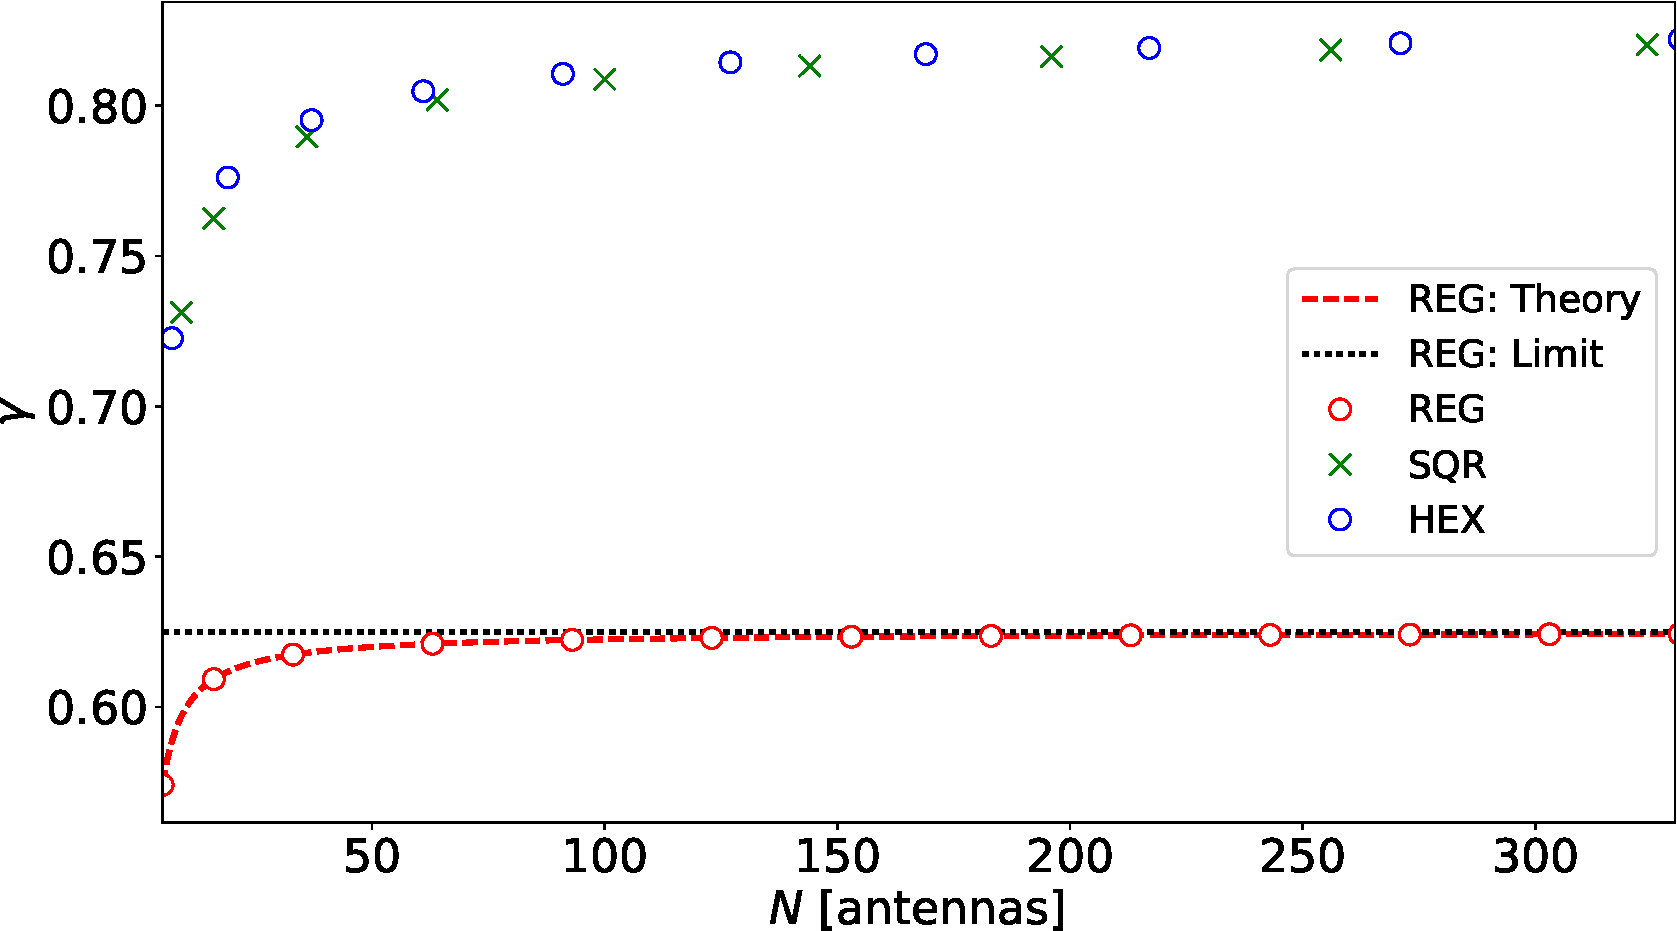
\includegraphics[width=0.47\textwidth]{./sparsity.pdf}\label{fig:gamma}}
% V_R_3.pdf: 585x441 pixel, 72dpi, 20.64x15.56 cm, bb=0 0 585 441
\subfigure[$c$]{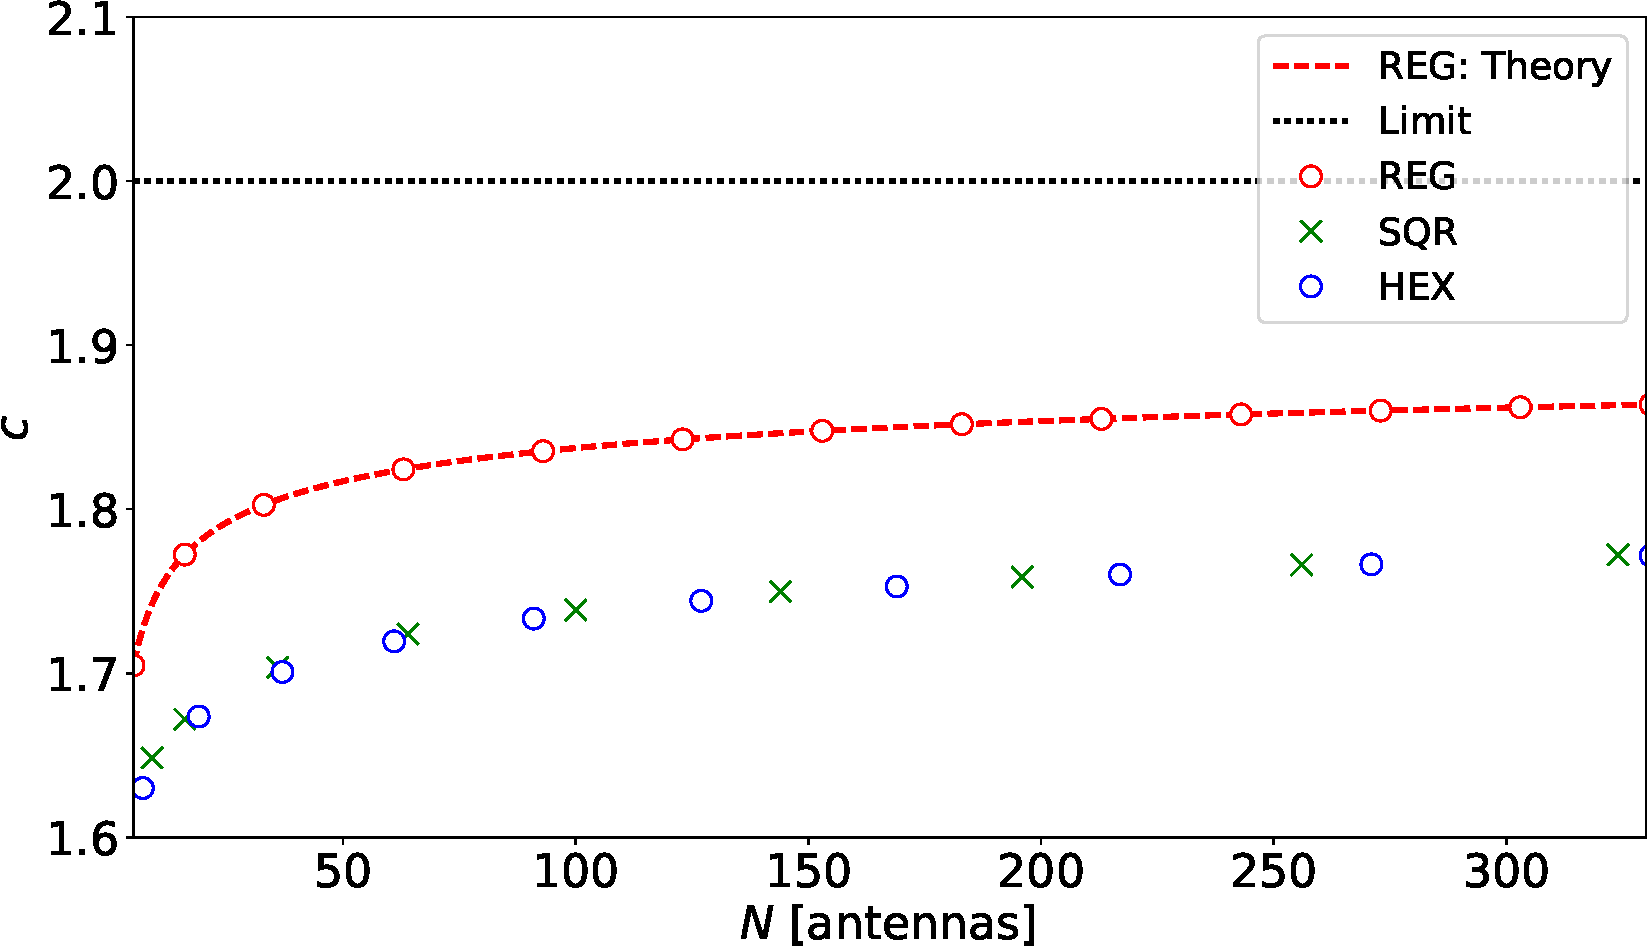
\includegraphics[width=0.46\textwidth]{./comp_order.pdf}\label{fig:c}}
\caption{In the left panel we plot the sparsity ratio $\gamma$ (the number of zero entries relative to the total number of entries in a matrix) of the modified Hessian $\bmH$ as a function of the number 
of antennas $N$ in the array for different geometries, namely an hexagonal grid (blue circles), a square grid (green crosses) and a regular east-west grid (red circles). For the regular east-west grid we are able to construct an analytical expression for $\gamma$ (the dashed red line). Taking the limit 
of this analytic expression produces the black dotted line. In the right panel we plot the order of the computational cost $c$ for inverting $\bmH$ as a function of the number 
of antennas in the array for different geometries. We use the same color scheme in the right and left panels. The red dashed line 
in the right panel is associated with the theoretical curve of $c$ we computed for the east-west regular grid. The limit of the red-dashed curve is two, which we 
have plotted with a black dotted line.
\label{fig:sparsity}} 
\end{figure*}

\section{Comparison Results}
\label{sec:comparison}
We are now in a position to make a final comparison between redundant \textsc{StEFCal} and the PCG method. Inverting $\bmH$ by assuming it is a diagonal matrix (i.e. using redundant \textsc{StEFCal}) is computationally inexpensive, while inverting $\bmH$ using PCG is more computationally taxing. On the other hand, one inversion with PCG is much more 
accurate than using an approximate inverse. The question is now, if the inverse using the PCG method is much more accurate will the LM implementation using it require fewer iterations than redundant \textsc{StEFCal} requires. Moreover, will the number 
of LM iterations PCG requires be so few that it manages to outperform redundant \textsc{StEFCal} in the end. To answer this we need to compute the number of approximate Hessian inversions $k$, redundant \textsc{StEFCal} computes, in the same time it takes PCG to perform a single Hessian inversion.
We can compute this with
\begin{align}
\label{eq:k} 
 kP &\approx P^{1.7}, & k &\approx P^{0.7}.
\end{align}
Next we need to measure the number of LM iterations we save by using the PCG method and compare it to equation~\ref{eq:k}. We make this comparison 
in Fig.~\ref{fig:out_diff}. Fig.~\ref{fig:out_diff} tells us that redundant \textsc{StEFCal} will outperform the PCG method as the number of LM iterations we save by taking the 
full inverse is not enough to exceed $k$. In this comparison we have only taken into account the cost of inverting $\bmH$. The PCG method, however, is still 
useful in practice as it would be more straightforward to apply it to other calibration use cases.

\begin{figure*}
\centering
\subfigure[Number of LM iterations required by redundant \textsc{StEFCal} and PCG.]{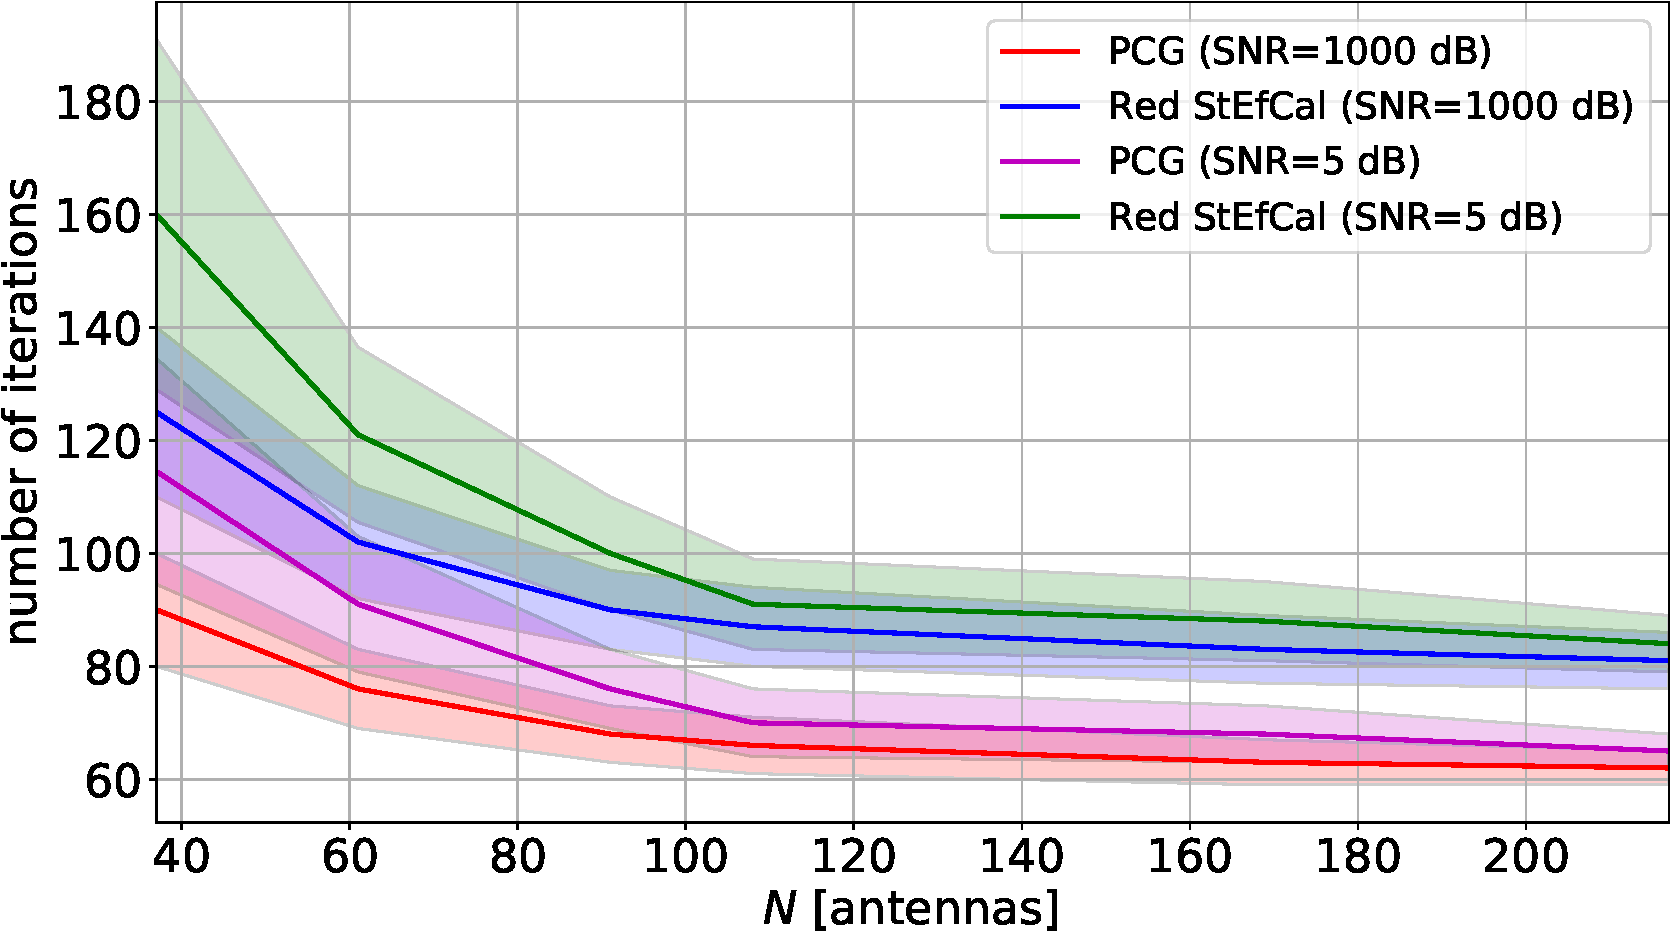
\includegraphics[width=0.47\textwidth]{./outerloop.pdf}\label{fig:outerloop}}
% V_R_3.pdf: 585x441 pixel, 72dpi, 20.64x15.56 cm, bb=0 0 585 441
\subfigure[Difference.]{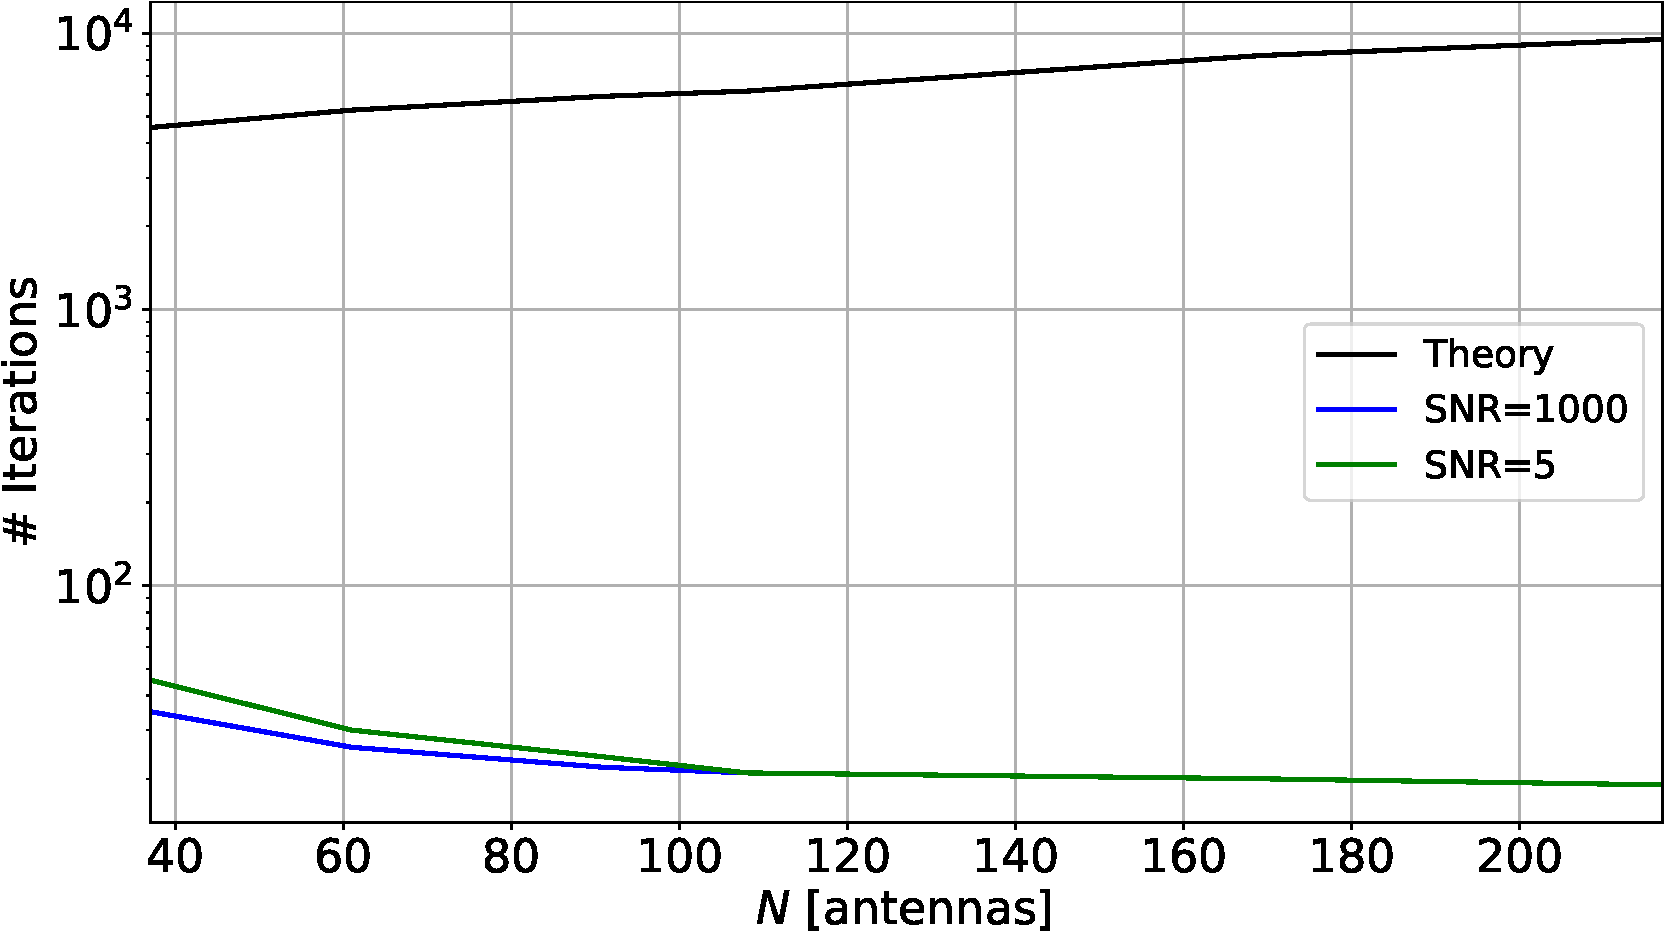
\includegraphics[width=0.47\textwidth]{./diff.pdf}\label{fig:diff}}
\caption{The graphs presented here were generated using the second experimental setup in Table~\ref{tab:ch_parm}. In the left panel we have the number of LM iterations 
that is required by redundant \textsc{StEFCal} (green and blue curve) and the PCG (magenta and red curve) method to converge to a parameter error tolerance of 1e-6 whilst using different 
SNR values as a function of the number of antennas $N$ in the array. In the right panel we have the average amount of LM iterations (difference between the redundant \textsc{StEFCal} and PCG curves in the left panel) we save (green and blue curve) by computing the full-inverse with the PCG method whilst using different SNR values.
The black curve is associated with $k$, the number of LM iterations redundant \textsc{StEFCal} can perform in the same time it takes the LM implementation using 
the PCG method to perform one iteration.
\label{fig:out_diff}} 
\end{figure*}

%\subsubsection{Simplifying GN}

% The 
% normal skymodel-based equivalent of equation~\ref{eq:two_thrids} is equal to \citep{Smirnov2015}:
% \begin{equation}
% \label{eq:one_half}
% \breve{\bg}_{k+1} = (\bJ^H\bJ)^{-1}\bJ^H\breve{\bd} + \frac{1}{2}\breve{\bg}_{k}, 
% \end{equation}
% where $\breve{\bg} = [\bg^T,\conj{\bg}^T]^T$
% 
% FIX TRANSPOSE PROBLEM

%\section{Comparing ADI and PCG}
%\section{Implementation} 
% \section{Redundant \textsc{StEfCal}}
% \label{sec:results}
% In Section~\ref{sec:red_wirtinger} we discussed the complex GN and LM algorithms and how they relate to redundant calibration. If we inspect equation~\ref{eq:GN_update} and 
% equation~\ref{eq:LM_update} we see that the most expensive operation used by the GN and LM algorithms is the inversion of the Hessian, $\bH$. The most logical 
% way of speeding up the algorithm is to investigate whether we can do this inversion in some efficient way.
% 
% Two recent algorithms have been proposed that are able to invert $\bH$ in an efficient manner, namely the ADI \citep{Marthi2014} and PCG \citep{Liu2010} methods. 
% Note that here we focus solely on comparing the computational complexity of inverting $\bH$ using either one of these two methods. Rating the LM or GN algorithms
% using one of these approaches relative to each other once the computational complexity of inverting $\bH$ is known is trivial. The simulations we performed to compare these two 
% methods are summarized in Section~\ref{sec:simulations}.
% 
% %We restrict ourselves to comparing the most 
% %expensive operation of the two methods namely, computing the inverse of the Hessian $\bH$ (or modified Hessian $\bmH$ in the case of LM). It becomes trivial to rate these two 
% %algorithms relative to each other once the computational complexity of the inverse operation is known. 
% 
% The basic difference between these two speedup algorithms can be understood by inspecting Fig.~\ref{fig:hessian}. The first observation we can make by inspecting 
% Fig.~\ref{fig:hessian_reg} and Fig.~\ref{fig:hessian_hex} is that the diagonal entries of $\bH$ are more significant than the off-diagonal entries in both cases.
% It therefore makes sense to approximate the $\bH$ with its diagonal, which greatly simplifies the computational complexity of inverting 
% $\bH$, i.e. it becomes $\mathbb{O}(P)$\footnote{The cost of constructing 
% the diagonal is not included in this estimate.} \citep{Smirnov2015}. This diagonal-approximation approach is effectively ADI \citep{Marthi2014}. The exact details of why this 
% is the case is discussed in Section~\ref{sec:adi}. We will also show how \citet{Marthi2014}, \citet{Smirnov2015} and \citet{Salvini2014} relate to each other in that same section. It should be noted here that strictly speaking the ADI method actually refers to the complete LM update step using the approximate $\bH$ and not just 
% to the inversion of the approximate $\bH$. To improve the readability of the paper, we use the acronym ADI to refer to both the faster approximate inverse approach and the complete LM algorithm that uses it.
% Which one of these two concepts we are actually referring to, however, is always perfectly clear from the context.
% %Furhtermore, the name ADI also implies that with this algorithm we alternate between computing the 
% %gains, their conjugates and the true observed visibilities. %In Appendix~\ref{sec:sbc} we briefly summarize the ADI method that is used for skymodel-based calibration.
% 
% The second observation we can make from Fig.~\ref{fig:hessian_reg} and Fig.~\ref{fig:hessian_hex} is that both Hessians contain many zero entries, i.e. they are sparse matrices. This, in conjunction with the more significant diagonal entries, implies that the PCG method (presented in Section~\ref{sec:conj_grad}) 
% can be applied to invert them in a computationally efficient manner. \citet{Liu2010} proposed the PCG method to compute the inverse of $\bH$, however the computational complexity of this approach was not analyzed therein.  
% In Section~\ref{sec:pcg}, we do a proper computational complexity analysis of PCG. We find that the computational complexity of PCG is asymptotically bounded by $\mathbb{O}(P^2)$, which is 
% a lot better than straightforward inversion which takes $\mathbb{O}(P^3)$. 
% 
% 
% 
% %Since we approximate the Hessian in the ADI method with its diagonal the computational complexity of its inverse becomes $\mathbb{O}(P)$\footnote{The cost of constructing 
% %the diagonal is not included in this estimate.}. 
% 
% Even though the PCG method is computationally more expensive than the ADI method we cannot arrive at a final conclusion at this point. With the ADI method 
% we only approximate the inverse of the Hessian, while in the case of the PCG method we compute the exact inverse. So the question arises whether the LM algorithm using the PCG method 
% will converge much faster than the ADI method even though each iteration (which includes an inversion) is more expensive. We investigate this question in Section~\ref{sec:comparison}.
% 

% At this point there is no way of knowing if this is mere coincidence. DEF REWRITE THIS.
% 
% REWRTIE THIS IN A DIFFERENT WAY. START WITH CHENGULAR AND JUST MENTION THE LINK TO STEFCAL'S CHOICE OF ALPHA.
% 
% The update rules in equation~\ref{eq:lambda} and equation~\ref{eq:alpha} have been derived before, by Chengular... The approach they followed is discussed in the Appendix.
% 
% Interestingly enough, if we substitute $\alpha = 1$ into Eq.~\ref{eq:g_update} then it reduces to the skymodel-based StEFCal update rule. In Chengular they propose 
% an $\alpha = 0.3$.
% 
% In an attempt to merge the terminology that has independently develop in the general calibration and redundant calibration literature and to emphasize the close
% relationship between Stefcal and the approach derived by I will use the label Redunandat SteFCal (R-Stefcal) to refer to the NLS method proposed by ... 
% 
% ****\\
% 
% with $\alpha = \frac{1}{1+\lambda}$. Moreover $\lambda = \frac{1-\alpha}{\alpha}$. So in Marthi and Chengular (2014) they use an $\alpha$ of 0.3, which corresponds to an LM damping factor $\lambda$
% of $2\frac{1}{3}$.
% 
% NB:: NEED TO ADD SNR PLOTS HERE
% PLUS IMAGE OF HESSIAN FOR THE DISCUSSION






\section{Conclusion}
\label{sec:conclusions}
In Section~\ref{sec:red_wirtinger} we extended \textsc{StEfCal} to the redundant use case by using the Wirtinger formalism 
presented in \citet{Smirnov2015} (i.e. we presented redundant \textsc{StEfCal}). We also pointed out that redundant \textsc{StEfCal} was 
first derived by \citet{Marthi2014} under a different name using a different approach than the one used in this paper. In Appendix~\ref{sec:red_stef_ADI} we showed that redundant \textsc{StEfCal}
can also be derived using the ADI method. 

\citet{Liu2010} suggested to use the PCG method to speed-up redundant calibration. In Section~\ref{sec:pcg} we analyze the computational complexity of the PCG method when applied to the redundant calibration problem. 
In Section~\ref{sec:comparison} we do a comparison between redundant \textsc{StEfCal} and the PCG method. We found 
that although the PCG method does greatly imporove the speed of redundant calibration it does not outperform redundant \textsc{StEfCal}. 
% fiducial initial guess 
% 
% The following partial derivatives are now easily computed
% 
% \begin{eqnarray}
% \frac{c_{ij}}{\partial \eta_p} &=& y_{i-j} e^{\eta_p - i \varphi_p} e^{\eta_q - i \varphi_q}\\ 
% \frac{c_{ij}}{\partial \varphi_p} &=&  -i y_{i-j} e^{\eta_p - i \varphi_p} e^{\eta_q - i \varphi_q}\\
% \frac{c_{ij}}{\partial \eta_q} &=& y_{i-j} e^{\eta_p - i \varphi_p} e^{\eta_q - i \varphi_q}\\ 
% \frac{c_{ij}}{\partial \varphi_q} &=&  i y_{i-j} e^{\eta_p - i \varphi_p} e^{\eta_q - i \varphi_q}\\
% \frac{y_{i-j}}{\partial \varphi_q} &=&  e^{\eta_p - i \varphi_p} e^{\eta_q - i \varphi_q}
% \end{eqnarray}
% 
% 
% The Wirtinger derivative is used in the last equation.
% 
% \begin{eqnarray}
% c_{ij} &\approx& c_{ij}^0 + \Delta \eta_p(y_{i-j}^0 e^{\eta_p^0 - i \varphi_p^0} e^{\eta_q^0 - i \varphi_q^0}) + \Delta \eta_q(y_{i-j}^0 e^{\eta_p^0 - i \varphi_p^0} e^{\eta_q^0 - i \varphi_q^0})\\
% && -i\Delta\varphi_p (y_{i-j}^0e^{\eta_p^0 - i \varphi_p^0} e^{\eta_q^0 - i \varphi_q^0}) +i\Delta\varphi_q (y_{i-j}^0e^{\eta_p^0 - i \varphi_p^0} e^{\eta_q^0 - i \varphi_q^0})\\
% && y_{i-j}^1(y_{i-j}^0e^{\eta_p^0 - i \varphi_p^0} e^{\eta_q^0 - i \varphi_q^0})\\
% &\approx&  c_{ij}^0 + e^{\eta_p^0 - i \varphi_p^0} e^{\eta_q^0 - i \varphi_q^0}(y_{i-j}^1 + y_{i-j}^0( \Delta \eta_p+ \Delta \eta_q - i\Delta\varphi_p + i\Delta\varphi_p))
% \end{eqnarray}
% 
% \begin{equation}
% \label{eq:residual}
% r_{ij} = \delta_{ij} = c_{ij}-c_{ij}^0 = e^{\eta_p^0 - i \varphi_p^0} e^{\eta_q^0 - i \varphi_q^0}(y_{i-j}^1 + y_{i-j}^0( \Delta \eta_p+ \Delta \eta_q - i\Delta\varphi_p + i\Delta\varphi_p)) 
% \end{equation}
% 
% Eq.~\ref{eq:residual} allows us to construct the following linear system:
% 
% \begin{equation}
% \boldsymbol{J}[\boldsymbol{\Delta \eta},\boldsymbol{\Delta \varphi},\boldsymbol{\Delta y}]^T = \boldsymbol{r}, 
% \end{equation}
% 
% where $\boldsymbol{J}$ is equal to 
% \begin{equation}
% \boldsymbol{J} = \bigg [\overbrace{\frac{c_{pq}}{\partial \eta_p}}^{i= 1\cdots N},~\overbrace{\frac{c_{pq}}{\partial \varphi_p}}^{i= 1\cdots N},~\overbrace{\frac{c_{pq}}{\partial y_{t}}}^{t=1\cdots r_s} \bigg ] \bigg \} [pq] = 1\cdots N_{\textrm{b}} (p<q) 
% \end{equation}
% or
% \begin{equation}
% \boldsymbol{J} = \bigg [\frac{c_{pq}}{\partial \boldsymbol{\eta}},~\frac{c_{pq}}{\partial \boldsymbol{\varphi}},~\frac{c_{pq}}{\partial \boldsymbol{y}} \bigg ] \bigg \} [pq] = 1\cdots N_{\textrm{b}} (p<q). 
% \end{equation}
% 
% The last column is again a Wirtinger derivative.
% 
% Which means we can obtain the least-squares estimate as follows:
% 
% \begin{equation}
% [\boldsymbol{\Delta \eta},\boldsymbol{\Delta \varphi},\boldsymbol{\Delta y}]^T = [\boldsymbol{J}^H\boldsymbol{J}]^{-1}\boldsymbol{J}^H\boldsymbol{r}.
% \end{equation}




\bibliographystyle{mn2e}
\bibliography{paperG2}

\appendix

\section{Simulations}
\label{sec:simulations}
\begin{table*}
\centering
\caption{The following fixed simulation parameters were used to generate the results of this paper. We use $U$ to represent 
a uniform distribution.}
\begin{tabular}{|c c c c c c c|} 
\hline
Declination & Latitude & Minimum baseline & Geometry& Sources & Flux & Spatial \\
\hline 
\hline
 $-74^{\circ}39'37.481''$ & $-30^{\circ}43'17.34''$ & 20 & Hexagonal &100 & Pareto (shape param. of 2) & $U[-3,3]$ (deg.) 
\end{tabular}
\label{tab:fixed_parm}
\end{table*}

\begin{table*}
\centering
\caption{The gain error models used in this paper. We have used the symbol $x$ here as a proxy as it can either refer to time-slots or channels. We either
performed our simulations over multiple time-slots and one frequency channel or one timeslot and multiple frequencey channels (see Table~\ref{tab:ch_parm}). Moreover, $c$ in the left most column denotes the speed of light.}
\begin{tabular}{|c c c c|} 
\hline
Number tag & 1 & 2 & 3\\
Model & Sinusoidal: amplitude and phase & Sinusoidal: real and imaginary parts & Linear phase slope \\ [0.5ex] 
\hline\hline
Function & $(A+1)e^{jP}$ & $A\cos(2\pi fx+B)+1.5A+jC\sin(2\pi fx+D)$ & $e^{jP}$ \\ 
\hline
Parameters & $A=a\cos(2\pi fx +b)$  & $f=5$ & $P=\tau x$ \\
 & $P =c \cos(2\pi fx +d)$ & $A,C\sim U[0.5,10]$ & $\tau = \frac{l}{c}$ \\
 & $f=5$ & $B,D\sim U[0,2\pi]$ &  $l\sim U[5,50]$ (m)\\
 & $a\sim U[0.8,0.9]$ &  & \\ 
 & $c\sim U[0.5,5]$ &  &  \\ 
 & $b,d\sim U[0,2\pi]$ &  &  \\ 
\hline
\end{tabular}
\label{tab:gain_parm}
\end{table*}

\begin{table}
\centering
\caption{We generated results using two major experimental setups. We either used one frequency channel and multiple time-slots, or one time-slot and multiple frequency 
channels. The most important parameters used in realizing these two major setups are presented here. Note that we refer to the gain error models in Table~\ref{tab:gain_parm} in the 
last row of this table.}
\begin{tabular}{|c c c|} 
\hline
 & Setup 1 & Setup 2\\
\hline
\hline
 Num. channels & 1024 & 1\\
$\nu$-range & 100-200 MHz & 1.4 GHz\\
Num. timeslots & 1 & 50\\
%Hour angle &-1^h & [-1^h,1^h]\\
Gain error model (Table~\ref{tab:gain_parm}) & 2 & 1\\
%Initial guess: $\bz_0$ & $\bone$ & $\bone$\\
\hline
\end{tabular}
\label{tab:ch_parm}
\end{table}
%The main purpose of the simulations conducted in this paper is to genrate experimental results with which we can compare the computational complexity of ADI and PCG. We used an hexagonal geometric layout with an adjustable number of rings during the 
%simulations. 
In this section we describe the simulations we performed to generate the results we report in the paper. We first discuss some 
of the simulation parameters we used followed by the general flow of the simulations that were conducted.

For the skymodel we generated 100 flat spectrum sources. Each source had a random flux value and position. The flux of the sources followed a Pareto distribution (with a shape parameter of 2), while their positions were uniformly 
distributed in a 3$^{\circ}$ by 3$^{\circ}$ square grid around the field center. The remaining fixed simulation parameters can all be found in Table~\ref{tab:fixed_parm}. 
We also employed three different gain error models which we summarize in Table~\ref{tab:gain_parm}. We found that it did not matter which gain error model we used during
our simulations, as the model we used did not have an impact on the results. Moreover, we had two major experimental setups, we either made use of simulated observations consisting of one frequency channel and multiple time-slots or one time-slot and multiple channels.
We describe these two experimental setups in more detail in Table~\ref{tab:ch_parm}. As was the case for the gain error models, the experimental setup 
that was used did not alter the simulation results. 

The main flow of a single simulation is as follows. We created corrupted visibilities using the fixed simulation parameters presented in Table~\ref{tab:fixed_parm} and either one of the experimental setups summarized in Table~\ref{tab:ch_parm}. We then used per time-slot and channel redundant calibration, i.e. we use the LM algorithm, which in turn makes use of either the ADI or PCG method, to 
estimate the gains and the true observed visibilities. Our initial parameter guess $\bz_0$ was chosen to be an all one vector. To obtain statistically significant results we performed, for both the ADI and PCG methods, multiple statistical independent simulations. 

Furthermore, the following SNR definition is used in this paper  
\begin{equation}
\label{}
\textrm{SNR} = \frac{<\bv\odot\conj{\bv}>_{\nu,t,pq}}{<\bn\odot\conj{\bn}>_{\nu,t,pq}}, 
\end{equation}
where $<*>_{\nu,t,pq}$ denotes averaging over frequency, time and baseline. The definition we use here is based on the SNR definitions used in \citet{Liu2010} and \citet{Marthi2014}.



\section{\textsc{LOGCAL}}
\label{sec:logcal}
We can rewrite equation~\ref{eq:vis_red} to \citep{Liu2010}
\begin{eqnarray}
\ln |d_{pq}| &=& \ln |g_p| + \ln |g_q| + \ln |y_{\phi_{pq}}| + s_{pq} \label{eq:logcal_amp}\\
\angle d_{pq} &=& \angle g_p - \angle g_q + \angle \phi_{pq} + t_{pq} \label{eq:logcal_phase}
\end{eqnarray}
where
\begin{align}
s_{pq} &= \mathscr{R} \left \{1 + \frac{n_{pq}}{g_p\conj{g_q}y_{\phi_{pq}}} \right \}, & t_{pq} &= \mathscr{I}\left \{1 + \frac{n_{pq}}{g_p\conj{g_q}y_{\phi_{pq}}} \right \}.
\end{align}
Moreover, $\mathscr{R}\{*\}$ and $\mathscr{I}\{*\}$ denote the real and imaginary operators. 

With the aid of equation~\ref{eq:logcal_amp} we can construct the following linear system:
\begin{equation}
\label{eq:log_system}
\bdelta = \bJ\bzeta + \bs, 
\end{equation}
where
\begin{align}
\left [ \bdelta \right ]_{\alpha_{pq}} &= \ln |d_{pq}|, & \left [ \bs \right ]_{\alpha_{pq}} = s_{pq} 
\end{align}
and
\begin{equation}
\left [ \bzeta \right ]_{j} = \begin{cases} \ln |g_j| & \textrm{if}~j\leq N \\ \ln |y_{j-N}| & \textrm{otherwise} \end{cases}. 
\end{equation}
Furthermore,
\begin{equation}
\bJ = 
\begin{bmatrix}
\bN & \bM
\end{bmatrix}
\end{equation}
with 
\begin{equation}
[\bN]_{\alpha_{pq},j} = \begin{cases}
       1 & \textrm{if}~(p=j)~\textrm{or}~(q=j)\\
       0 & \textrm{otherwise}
      \end{cases}
\end{equation}
and
\begin{equation}
[\bM]_{\alpha_{pq},j} = \begin{cases}
       1 & \textrm{if}~\phi_{pq}=j\\
       0 & \textrm{otherwise}
      \end{cases}
\end{equation}

The least squares solution to Eq.\ref{eq:log_system}, under the incorrect assumption that $s_{pq}$ is normally distributed, is given by
\begin{equation}
\bzeta = (\bA^T\bA)^{-1} \bA^T\bdelta. 
\end{equation}
How to correctly deal with the fact that $s_{pq}$ is not normally distributed is discussed in \citep{Liu2010}. A similar linear system can be constructed for equation~\ref{eq:logcal_phase}. 
From the least squares solutions to the linear systems associated with equation~\ref{eq:logcal_amp} and equation~\ref{eq:logcal_phase} we can compute the antenna gains as well as the true visibilities.

\section{\textsc{lincal}}
\label{sec:lincal}
Assume that $\eta_p,\eta_q,\widetilde{\eta}_{\phi_{pq}},\varphi_p,\varphi_q$ and $\widetilde{\varphi}_{\phi_{pq}}$ are real valued variables.
We can rewrite equation~\ref{eq:vis_red_vec} to \citep{Liu2010}
\begin{equation}
\label{eq:lincal_vec}
\bd = \bv(\bvarrho) + \bn, 
\end{equation}
where 
\begin{align}
\left [ \bv(\bvarrho) \right ]_{\alpha_{pq}} &= e^{\eta_p - i \varphi_p} e^{\widetilde{\eta}_{\phi_{pq}}- i \widetilde{\varphi}_{\phi_{pq}}} e^{\eta_q + i \varphi_q}\\
&= v_{pq},
\end{align}
and
\begin{equation}
\bvarrho = 
\begin{bmatrix}
\bmath{\eta} \\
\bvarphi \\
\widetilde{\bmath{\eta}} \\
\widetilde{\bvarphi}
\end{bmatrix},\qquad
\begin{aligned}
\bmath{\eta} &= [\eta_1, \eta_2,\cdots \eta_N]^T\\
 \bmath{\varphi} &= [\varphi_1, \varphi_2,\cdots \varphi_N]^T\\
 \widetilde{\bmath{\eta}} &= [\widetilde{\eta}_1, \widetilde{\eta}_2,\cdots \widetilde{\eta}_L]^T\\
 \widetilde{\bmath{\varphi}} &= [\widetilde{\varphi}_1, \widetilde{\varphi}_2,\cdots \widetilde{\varphi}_L]^T
\end{aligned}.
\label{eq:help}
\end{equation}
Note that the vectors $\bmath{\eta},~\bvarphi,~\widetilde{\bmath{\eta}}$ and $\widetilde{\bvarphi}$ are real valued.

The first order Taylor expansion of equation~\ref{eq:lincal_vec} around the fiducial point $\bvarrho_0$ is equal to
\begin{equation}
\label{eq:d_lin}
\bd = \bv_0 + \bmJ_0 \Delta \bvarrho  + \bn.
\end{equation}
If we calculate the residual, dropping the reference to a specific fiducial point, we obtain: 
\begin{equation}
\label{eq:r_lin}
\br = \bd - \bv = \bmJ \Delta \bvarrho + \bn.
\end{equation}
Moreover,
\begin{equation}
\label{eq:jac_upper_lincal}
\bmJ = \begin{bmatrix}
       \bN & \bM 
       \end{bmatrix},
\end{equation}
where
\begin{align}
\bN &= \begin{bmatrix} \bO & \bP \end{bmatrix}, & \bM &= \begin{bmatrix} \bQ & \bR \end{bmatrix}, 
\end{align}
\begin{equation}
 [\bO]_{\alpha_{pq},j} =  \frac{\partial v_{pq}}{\partial \eta_j} = \begin{cases} 
    v_{pq} &\textrm{if}~(p=j)~\textrm{or}~(q=j)\\
    0 & \textrm{otherwise}
   \end{cases},
\end{equation}
\begin{equation}
 [\bP]_{\alpha_{pq},j} =  \frac{\partial v_{pq}}{\partial \varphi_j} = \begin{cases}
                                                                        i v_{pq} &\textrm{if}~ p=j\\
                                                                        -i v_{pq} &\textrm{if}~ q=j \\
                                                                        0 & \textrm{otherwise} 
                                                                       \end{cases}
\end{equation}
\begin{equation}
 [\bQ]_{\alpha_{pq},j} =  \frac{\partial v_{pq}}{\partial \widetilde{\eta}_j} = \begin{cases} 
    v_{pq} &\textrm{if}~\phi_{pq}=j\\
    0 & \textrm{otherwise}
   \end{cases},
\end{equation}
\begin{equation}
 [\bR]_{\alpha_{pq},j} =  \frac{\partial v_{pq}}{\partial \widetilde{\varphi}_j} = \begin{cases} 
    i v_{pq} &\textrm{if}~\phi_{pq}=j\\
    0 & \textrm{otherwise}
   \end{cases}.
\end{equation}
Augmenting the residual by taking into account its conjugate results in 
\begin{equation}
\breve{\br} = \bJ \Delta \bvarrho + \bn, 
\end{equation}
where $\breve{\br} = \begin{bmatrix}\br^T & \conj{\br}^T \end{bmatrix}^T$ and 
\begin{equation}
\label{eq:Jac_lin}
\bJ = 
\begin{bmatrix}
 \bmJ\\  
 \conj{\bmJ}
\end{bmatrix}.
\end{equation}
The solution to 
\begin{equation}
 \min_{\Delta \bvarrho} \| \breve{\br} - \bJ \Delta \bvarrho\|_F^2,
\end{equation}
is equal to 
\begin{equation}
\label{eq:LINCAL_update}
\Delta \bvarrho = (\bJ^H\bJ)^{-1} \bJ^H\breve{\br}. 
\end{equation}
equation~\ref{eq:LINCAL_update} is used to iteratively determine a new estimate of the parameter vector $\bvarrho$ as follows
\begin{equation}
\label{eq:new_rho}
\bvarrho_{k+1} = \bvarrho_k + \Delta \bvarrho_k. 
\end{equation}
Note that we do not explicitly denote the $k$ index in equation~\ref{eq:LINCAL_update}.
Moreover, equation~\ref{eq:LINCAL_update} is the GN update associated with the following minimization problem \citep{Kurien2016}
\begin{equation}
\label{eq:least_squares_lincal}
\min_{\bmath{\varrho}} \|\breve{\br}\| = \min_{\bmath{\varrho}} \|\breve{\bd} - \breve{\bv}(\bmath{\varrho})\|.
\end{equation}

\section{Conjugate Gradient Method}
\label{sec:conj_grad}
The CG method was independently discovered by \citet{Hestenes1973} and \citet{Stiefel1952}. They later published a joint paper, which is now considered as the seminal
reference on CG \citep{Hestenes1952}. The iterative CG method is used to solve a particular class of linear system. The CG method is generally used to solve
\begin{equation}
\label{eq:linear_system}
\bb = \bA\bx,
\end{equation}
where $\bb\in\mathbb{C}^P$ is a known complex column vector of size $P$, $\bx\in\mathbb{C}^P$ is an unknown complex column vector with the same length as $\bb$, and $\bA\in\mathbb{C}^{P\times P}$ is a square positive-definite Hermitian matrix with the appropriate dimensions.  
Moreover, using the CG method to solve equation~\ref{eq:linear_system} will only be computationally advantageous if $\bA$ is also sparse (contain many zero entries).
Using the iterative CG method to solve large sparse linear sytems was popularized by \citet{Reid1971}. A good tutorial on the CG method can be found in \citep{Shewchuk1994}.
The iterative CG method is presented in Algorithm \ref{algo:CG}. 

%If $\bA$ is a square positive semi-definite Hermitian matrix, then the conjugate gradient method only converges if $\bb$ is in the column range of $\bA$ (cite Lu2016).

%\begin{algorithm}
%\caption{Conjugate Gradient Method. Inputs: $\bA$, $\bb$, a starting value for $\bx$, maximum number of iterations $k_{\textrm{max}}$ and an error tolerance $\epsilon<1$ Output: $\bx$ the solution to equation~\ref{eq:linear_system}. \citep{Shewchuk1994}.}\label{algo:CG}
%\begin{algorithmic}[1]
%\State $k \gets 0$
%\State $\br \gets \bb - \bA\bx$
%\State $\bp \gets \br$
%\State $\delta_{\textrm{new}} \gets \br^H\br$
%\State $\delta_0 \gets \delta_{\textrm{new}}$
%\While{$k\leq k_{\textrm{max}}$ and $\delta_{\textrm{new}} > \epsilon^2\delta_0$}
%\State $\alpha \gets \frac{\delta_{\textrm{new}}}{\bp^H\bA\bp}$
%\State $\bx \gets \bx + \alpha\bp$
%\State $\br \gets \br - \alpha\bA\bp$
%\State $\delta_{\textrm{old}} \gets \delta_{\textrm{new}}$ 
%\State $\delta_{\textrm{new}} \gets \br^H\br$
%\State $\beta \gets \frac{\delta_{\textrm{new}}}{\delta_{\textrm{old}}}$
%\State $\bp \gets \br + \beta\bp$
%\State $k \gets k + 1$
%\EndWhile
%\end{algorithmic}
%\end{algorithm}

\subsection{Computational Complexity}
\citet{Kaniel1966} was able to determine convergence bounds for CG using Chebyshev polynomials. A much more in depth analysis of CG convergence can be found in
\citep{Sluis1986}. As can be seen from Algorithm \ref{algo:CG}, the CG method makes use of a major outer loop (line 6 of Algorithm \ref{algo:CG}). It turns out that at worst 
the number of major iterations that CG requires to converge\footnote{If the $\bA$-norm is used to calculate the error.} is proportional to $\sqrt{\kappa}$, where $\kappa$ is the spectral condition number of the matrix $\bA$.
The mathematical definition of $\kappa(\bA)$ is
\begin{equation}
\label{eq:kappa}
\kappa(\bA) = \frac{\lambda_{\textrm{max}}}{\lambda_{\textrm{min}}}, 
\end{equation}
where $\lambda_{\textrm{max}}$ and $\lambda_{\textrm{min}}$ respectively denote the largest and the smallest eigenvalue of $\bA$.
Moreover, the most expensive operation that is conducted within each major loop of Algorithm~\ref{algo:CG} is the vector-matrix product $\bA\bp$, which has a complexity of $\mathbb{O}(m)$, where $m$ is the number of non-zero entries in $\bA$.
The computational complexity of CG is therefore 
\begin{equation}
\label{eq:cg_bound}
\mathbb{O}(\sqrt{\kappa}m). 
\end{equation}
It should now also be clear to the reader why the CG method is especially applicable to sparse linear systems. In sparse linear systems $m < P^2$.

\subsection{Preconditioning}
\label{sec:precon}
Preconditioning is a technique which allows us to improve the condition number of a matrix. Let $\bM$ be a positive-definite Hermitian matrix.
We can now indirectly solve for $\bx$ by using 
\begin{equation}
\label{eq:prec}
\bM^{-1}\bA\bx = \bM^{-1}\bb.
\end{equation}
If $\bM$ is a good preconditioner then $\kappa(\bM^{-1}\bA) \ll \kappa(\bA)$, i.e. a good preconditioner lowers the condition number of a matrix which in turn increases the convergence speed 
of CG (see equation~\ref{eq:cg_bound}). In this paper, we denote matrix inversion with $(*)^{-1}$. The best possible choice of $\bM$ would therefore be $\bA$, which would lead to $\kappa$ becoming unity (as the largest and smallest eigenvalue of the identity matrix are equal to one).
If $\kappa$ is one then equation~\ref{eq:cg_bound} simplifies and becomes $\mathbb{O}(m)$. However, if we knew the inverse of $\bA$ then obtaining $\bx$ would be trivial and there would be no need for the CG method in the first place. 
In short, a good preconditioner $\bM$ must approximate $\bA$ fairly accurately. However, if it is not much less expensive to 
compute the inverse of $\bM$ than that of $\bA$ we actually gain nothing (see equation~\ref{eq:prec}).  

If the diagonal entries of $\bA$ are much more significant than its off-diagonal entries then the 
Jacobian preconditioner is a good choice of $\bM$. The Jacobian preconditioner is computed as follows:
\begin{equation}
\bM = \bA\odot\bI, 
\end{equation}
where $\bI$ is the identity matrix and $\odot$ denotes the Hadamard product. Since the Jacobian preconditioner is a diagonal matrix its inverse can be obtained trivially.

\subsection{Normal Equation}
\label{sec:normal}
Lets assume that instead of equation~\ref{eq:linear_system} we have a more general linear system, i.e.
\begin{equation}
 \bb = \bB\bx,
\end{equation}
where $\bb\in\mathbb{C}^K$, $\bx\in\mathbb{C}^P$  and $\bB\in\mathbb{C}^{K \times P}$, with $K > P$. We can use the normal equation 
\begin{equation}
\label{eq:normal_equation}
\bB^H\bB\bx = \bB^H\bb, 
\end{equation}
to estimate the $\bx$ that minimizes
\begin{equation}
\label{eq:norm_ls}
\|\bb-\bB\bx\|_F^2. 
\end{equation}
In this paper, we denote the Hermitian transpose with $(*)^H$ and the Frobenius norm with $\|*\|_F$.

There are a few important observations that we can make while inspecting equation~\ref{eq:normal_equation}:
\begin{enumerate}
\item $\bB^H\bB$ is a square positive semi-definite Hermitian matrix by construction.
\item $\bB^H\bb$ is in the column range of $\bB^H\bB$; this follows trivially from 
\begin{equation}
\bB^H\bb \in \mathcal{R}(\bB^H) \implies \bB^H\bb \in \mathcal{R}(\bB^H\bB).   
\end{equation}
\end{enumerate}
In this paper, we denote the column range of a matrix $\bA$ with $\mathcal{R}(\bA)$.

Recall that we mentioned that in general we can only solve equation~\ref{eq:linear_system} with CG if $\bA$ is a square positive-definite Hermitian matrix. The CG method actually has an even broader applicability: it can be used to solve equation~\ref{eq:linear_system} even if $\bA$ is a Hermitian positive semi-definite
square matrix as long as $\bb$ is in the column range of $\bA$ \citep{Lu2015}. In light of \citet{Lu2015}, the two observations in the numbered list we presented in the previous paragraph imply that equation~\ref{eq:normal_equation}
can be solved by employing the CG method. The solution returned by CG is, however, only unique if $\bB^H\bB$ is positive-definite (invertible). The solution
obtained by CG, whether it is unique or not, does minimize equation~\ref{eq:norm_ls} in a least squares sense.

Note that if $\bA$ is positive semi-definite, its smallest eigenvalue is zero. This implies that equation~\ref{eq:kappa} is not defined. \citet{Lu2015} show that when $\bA$
is a square positive semi-definite Hermitian matrix we do not use the spectral condition number to bound the convergence complexity of CG, but the general spectral condition
number instead. The general spectral condition number is very similar to the spectral condition number; the only difference being that in equation~\ref{eq:kappa} we replace  
$\lambda_{\textrm{min}}$ with $\lambda_{\textrm{min}}^+$, which denotes the smallest positive eigenvalue.


\section{Redundant Wirtinger Calibration - $\bJ$, $\bH$ and $\bJ^H\breve{\br}$}
\label{sec:analytic}
If we apply the definition in equation~\ref{eq:Jacobian} to equation~\ref{eq:least_squares_complex} we obtain the following analytic result:
\begin{equation}
\label{eq:Jacobian_red}
\bJ = \begin{bmatrix}
       \bM & \bN\\
       \conj{\bN} & \conj{\bM}
      \end{bmatrix},
\end{equation}
where
\begin{equation}
\bM =\begin{bmatrix}
      \bO & \bP
     \end{bmatrix},
\end{equation}
and 
\begin{equation}
\bN = \begin{bmatrix}
       \bQ & \bzero
      \end{bmatrix}.
\end{equation}
Moreover,
\begin{equation}
\left [ \bO  \right ]_{\alpha_{pq},j} = \begin{cases}
                                         y_{\phi_{pq}}\conj{g_q} & \textrm{if}~p=j\\
                                         0  & \textrm{otherwise} 
                                        \end{cases},
\end{equation}

\begin{equation}
\left [ \bP  \right ]_{\alpha_{pq},j} = \begin{cases}
                                         g_p\conj{g_q} & \textrm{if}~\phi_{pq}=j\\
                                         0  & \textrm{otherwise} 
                                        \end{cases}
\end{equation}
and
\begin{equation}
\left [ \bQ  \right ]_{\alpha_{pq},j} = \begin{cases}
                                         g_py_{\phi_{pq}} & \textrm{if}~q=j\\
                                         0  & \textrm{otherwise} 
                                        \end{cases}
\end{equation}

%\begin{align}
%\left [ \bM_1 \right ]_{\alpha_{pq},j} &= y_{\phi_{pq}}\conj{g_q}\delta_p^j, & \left [ \bM_2 \right ]_{\alpha_{pq},j} &= g_p\conj{g_q}\delta_{\phi_{pq}}^j 
%\end{align}
%\begin{equation}
%\left [ \bN_1 \right ]_{\alpha_{pq},j} = g_py_{\phi_{pq}}\delta^j_q. 
%\end{equation}
We use $\bzero$ to denote an all zero matrix. It is now trivial to compute the Hessian $\bH$ by using equation~\ref{eq:Jacobian_red}. If we substitute equation~\ref{eq:Jacobian_red} into $\bJ^H\bJ$
we obtain 
\begin{equation}
\label{eq:red_H}
\bH = \bJ^H\bJ = 
\begin{bmatrix}
\bA & \bB\\
\conj{\bB} & \conj{\bA}
\end{bmatrix},
\end{equation}
where

\begin{align}
\bA &= \begin{bmatrix} \bC & \bD\\ \bD^H & \bE \end{bmatrix}, & \bB &= \begin{bmatrix} \bF & \bG\\ \bG^T & \bzero \end{bmatrix},
\end{align}

\begin{equation}
[\bC]_{ij} = 
\begin{cases}
 \sum_{k \neq i} \left | g_k \right |^2 \left | y_{\zeta_{ik}} \right |^2 & \textrm{if} ~ i=j\\
 0 & \textrm{otherwise}
\end{cases},
\end{equation}
\begin{equation}
[\bD]_{ij} = 
\begin{cases}
 g_i \conj{y}_j  \left | g_{\psi_{ij}} \right |^2  & \textrm{if} ~ \psi_{ij}\neq0\\
 0 & \textrm{otherwise}
\end{cases},
\end{equation}

\begin{equation}
[\bE]_{ij} = 
\begin{cases}
 \sum_{rs \in \mathcal{RS}_i} \left | g_r \right |^2 \left | g_s \right |^2  & \textrm{if} ~ i=j\\
 0 & \textrm{otherwise}
\end{cases},
\end{equation}
\begin{equation}
[\bF]_{ij} = 
\begin{cases}
 g_i g_j  \left | y_{\zeta_{ij}} \right |^2  & \textrm{if} ~ i \neq j\\
 0 & \textrm{otherwise}
\end{cases},
\end{equation}
and
\begin{equation}
[\boldsymbol{G}]_{ij} = 
\begin{cases}
 g_i y_j  \left | g_{\xi_{ij}} \right |^2  & \textrm{if} ~ \xi_{ij}\neq0\\
 0 & \textrm{otherwise}
\end{cases}.
\end{equation}
Moreover, 
\begin{equation}
\mathcal{RS}_i = \left\{rs\in\mathbb{N}^2|(\phi_{rs} = i) \right\},
\end{equation}
\begin{equation}
\xi_{ij} = 
\begin{cases}
p~\textrm{if}~\exists! ~ p \in \mathbb{N} ~ s.t. ~(\phi_{pi} = j)\\
0~\textrm{otherwise}
\end{cases},
\end{equation}
and
\begin{equation}
\psi_{ij} = 
\begin{cases}
q~\textrm{if}~\exists! ~ q \in \mathbb{N} ~ s.t. ~(\phi_{iq} = j)\\
0~\textrm{otherwise}
\end{cases}.
\end{equation}


Furthermore, substituting equation~\ref{eq:Jacobian_red} into $\bJ^H\breve{\br}$ results in
\begin{equation}
\bJ^H\breve{\br} = \begin{bmatrix}
                   \ba \\
                   \bb \\
                   \conj{\ba}\\
                   \conj{\bb}
                   \end{bmatrix},
\end{equation}
where
\begin{align}
\label{eq:ab}
\left [ \ba \right ]_i &= \sum_{k\neq i} g_k \widetilde{y}_{ik}r_{ik},  & \left [ \bb \right ]_i &= \sum_{rs\in\mathcal{RS}_i}\conj{g}_r g_s r_{rs},
\end{align}
and
\begin{equation}
\widetilde{y}_{ik} = 
\begin{cases}
\conj{y}_{\zeta_{ik}} & \textrm{if}~k > i\\
y_{\zeta_{ik}} & \textrm{otherwise}
\end{cases}.
\end{equation}
Additionally, $\ba$ and $\bb$ are both column vectors. The lengths of $\ba$ and $\bb$ are $N$ and $L$ respectively.
The dimensions of the matrices we defined in this section are presented in Table~\ref{tab:matrix_dimensions}.

% \begin{equation}
% \boldsymbol{J}^H\breve{\boldsymbol{d}} = 
% \begin{bmatrix}
% \sum_{k\neq i } g_k x_{ik}d_{ik}\\
% \sum_{pq \in \mathcal{I}_j} \conj{g}_p g_q d_{pq}\\
% \downarrow^{*}
% \end{bmatrix}
% \begin{matrix}% matrix for right braces 
% \coolrightbrace{\sum g_k x_{\zeta_{ik}}d_{ik}}{i = 1\cdots N}\\
% \coolrightbrace{\sum \conj{g}_p g_q d_{pq}}{j = 1\cdots L}\\
% \vphantom{\downarrow^{*}}
% \end{matrix}
% \end{equation}

\begin{table}
\centering
\caption{The dimensions of the matrices defined in Section~\ref{sec:analytic}.}
\begin{tabular}{|c c|} 
\hline
Matrix & Dimension\\
\hline
\hline
$\bJ$ & $2B \times P$ \\
$\bM$ & $B \times (N+L)$ \\
$\bN$ & $B \times (N+L)$ \\
$\bO$ & $B \times N$ \\
$\bP$ & $B \times L$ \\
$\bQ$ & $B \times N$ \\
$\bzero$ & $B \times L$ \\
\hline
\hline
$\bH$ & $P\times P$\\
$\bA$ & $(N+L)\times (N+L)$\\
$\bB$ & $(N+L)\times (N+L)$\\
$\bC$ & $N \times N$\\
$\bD$ & $N \times L$\\
$\bE$ & $L \times L$\\
$\bF$ & $N \times N$\\
$\bG$ & $N \times L$\\
$\bzero$ & $L \times L$\\
\hline
\end{tabular}
\label{tab:matrix_dimensions}
\end{table}

\section{Simplifying GN}
\label{sec:simplify_GN}
The following identities,
\begin{align}
\label{eq:identities}
\frac{1}{3}\bJ\breve{\bz} &= \breve{\bv}, & \bJ^H\breve{\bv} &= \widetilde{\bH}\breve{\bz} 
\end{align}
are trivially established by mechanically showing that the left hand side of each identity in equation~\ref{eq:identities} is equal to its right hand side.
In equation~\ref{eq:identities}, $\widetilde{\bH}$ denotes $\bI\odot\bH$.

Replacing $\breve{\br}$ with $\breve{\bd}-\breve{\bv}$ in equation~\ref{eq:GN_update} results in
\begin{equation}
\label{eq:temp_GN_eq}
\Delta \breve{\bz} = (\bJ^H\bJ)^{-1}\bJ^H(\breve{\bd}-\breve{\bv}), 
\end{equation}
Substituting the first identity of equation~\ref{eq:identities} into equation~\ref{eq:temp_GN_eq} and simplifying the result 
\begin{equation}
\label{eq:one_thrid}
\Delta \breve{\bz} = (\bJ^H\bJ)^{-1}\bJ^H\breve{\bd}-\frac{1}{3}\breve{\bz}.
\end{equation}

\section{ADI}
\label{sec:red_stef_ADI}
The basic skymodel-based \textsc{StEfCal} update step is equal to  the leftmost term in equation~\ref{eq:g_update} (barring $\alpha$) \citep{Salvini2014}.
Assume without any loss of generality that the array is in an east-west regular grid. Furthermore, assume that $\boldsymbol{d}$ (see equation~\ref{eq:vis_red_vec}) has been re-ordered to
\begin{equation}
\widetilde{\boldsymbol{d}} = \left[d{12},\cdots,d_{N-1,N},d_{13},\cdots,d_{N-2,N},\cdots,d_{1N}\right]^T .
\end{equation}
The vector $\widetilde{\bn}$ should be interpreted in a similar manner.

equation~\ref{eq:vis_red_vec} can now be rewritten as 
\begin{equation}
\label{eq:linear_system}
\widetilde{\boldsymbol{d}} = \boldsymbol{J}\boldsymbol{y} + \widetilde{\bn}, 
\end{equation}
if we assume that $\boldsymbol{g}$ and its conjugate are known vectors. In equation~\ref{eq:linear_system},
\begin{equation}
\boldsymbol{J} = 
\begin{bmatrix}
g_1\conj{g}_2 & 0 & \cdots & 0\\
g_2\conj{g}_3 & 0 & \cdots & 0\\
\vdots & 0 & \cdots & 0\\
g_{N-1}\conj{g}_N & 0 & \cdots & 0\\
0 & g_1\conj{g}_3 & \cdots & 0\\
0 & \vdots & \cdots & 0\\
0 & g_{N-2}\conj{g}_N & \cdots & 0\\
0 & 0 & \cdots & 0\\
  & \vdots & \\
0 & 0 & \cdots & g_1\conj{g}_N\\  
\end{bmatrix}.
\end{equation}
We can now estimate $\boldsymbol{y}$ with
\begin{equation}
\label{eq:y_final}
\boldsymbol{y} = (\boldsymbol{J}^H\boldsymbol{J})^{-1}\boldsymbol{J}^H\widetilde{\boldsymbol{d}}, 
\end{equation}
where 
\begin{equation}
\label{eq:RHR}
[\boldsymbol{J}^H\boldsymbol{J}]_{ij} = 
\begin{cases}
\sum_{rs\in\mathcal{RS}_i} |g_r|^2|g_s|^2 &\textrm{if}~i=j\\
0&\textrm{otherwise}
\end{cases},
\end{equation}
and
\begin{equation}
\label{eq:RHd}
[\boldsymbol{J}^H\widetilde{\boldsymbol{d}}]_i = \sum_{rs\in\mathcal{RS}_i} \conj{g}_r g_s d_{rs}. 
\end{equation}
Substituting equation~\ref{eq:RHR} and equation~\ref{eq:RHd} into equation~\ref{eq:y_final} and then write out the analytic expression of $y_i$ we obtain
the leftmost term in equation~\ref{eq:y_update} (barring $\alpha$).


%We compare ADI with PCG in Section \textbf{??}, by using the results generated from the simulations we performed using 
%these two methods.

%The results reported in this paper were generated using two major experimental setups, namely a single time-slot and multiple frequency channels setup or 
%a single frquency channel and multiple time-slots setup. The simulation parameters which where kept fixed in both these setups can be found in 
%Table~\ref{tab:fixed_parm}. The sky-model we used to simulate the visibilities were the same for both setups.   We used a hexagonal redundant layout for our antenna positions. We produced 
%results for different 

\label{lastpage}
\end{document}


